\section{Function Approximation}

\subsection{Linear Approximation / Tangent Line Approximation}
Previously, we talked about how to find the equation of the tangent line for a function $f(x)$ at a given point $(a, f(a))$, which is:
\[y-f(a) = f'(a)(x-a)\]
or we can rewrite the expression and graph it:
\[y = \underbrace{f(a)}_{\text{starting value of }y} + \underbrace{f'(a)}_{\text{change rate of }y\text{ relative to }x} \cdot \underbrace{(x-a)}_{\text{deviation of }x\text{ from }a}\]

\begin{figure}[ht]
    \centering
    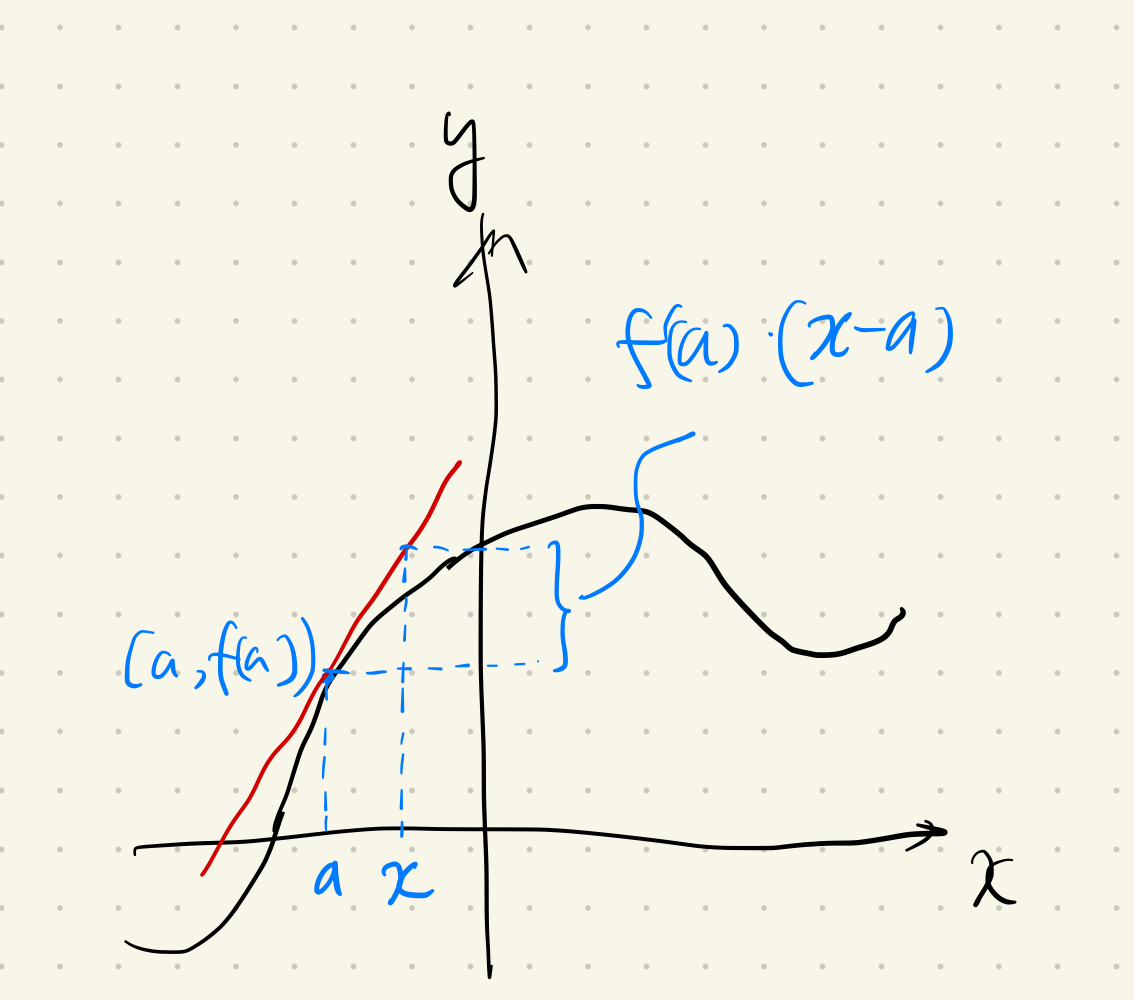
\includegraphics[width = 0.7\textwidth]{figures/chap 05/lin_approx_intro.png}
    \label{fig: lin_approx_intro}
\end{figure}

Since the curve is very close to the tangent line when $x$ is close to $a$, we can \textit{approximate} the values of $f(x)$ at $x \approx a$ with $\hat{f}(x) \approx f(a) + f'(a)(x-a)$.  In fact, one can prove that $\hat{f}(x)$ is the "best linear approximant" to $f(x)$ near $x=a$ by showing that any other linear approximant has a relatively larger error when $x \rightarrow a$.  To see this, say there is another linear approximant $f^*(x) = q + p(x-a)$, then ratio of the approximation errors between $\hat{f}(x)$ and $f^*(x)$ can be written as:

\[\frac{f(x)-\hat{f}(x)}{f(x) - f^*(x)} = \frac{f(x)-[f(a)+f'(a)(x-a)]}{f(x)-[q+p(x-a)]}\]

Taking the limit where $x \rightarrow a$, we yield:

\begin{align}
    &\lim\limits_{x \to a} \frac{f(x)-\hat{f}(x)}{f(x) - f^*(x)} \nonumber \\
    =&\lim\limits_{x \to a} \frac{f(x)-[f(a)+f'(a)(x-a)]}{f(x)-[q+p(x-a)]} \nonumber \\
    =&\lim\limits_{x \to a} \frac{[f(x)-f(a)]-f'(a)(x-a)}{[f(x)-f(a)]-[(q-f(a))+p(x-a)]} \label{eqn: lin_approx_best_1}\\
    =&\lim\limits_{x \to a} \frac{\frac{f(x)-f(a)}{x-a}-f'(a)}{\frac{f(x)-f(a)}{x-a}-\left[\frac{q-f(a)}{x-a}+p\right]}\label{eqn: lin_approx_best_2}
\end{align}

Now we have two cases:

\begin{enumerate}[(a)]
    \item If $q \ne f(a)$, then from (\ref{eqn: lin_approx_best_1}):\\
    \[\lim\limits_{x \to a} \frac{[f(x)-f(a)]-f'(a)(x-a)}{[f(x)-f(a)]-[(q-f(a))+p(x-a)]} = \frac{0-0}{0-[(q-f(a))-0]} = 0\]
    where $f(x)-f(a) = 0$ since $f(x)$ is differentiable at $x=a$ and thus continuous there.
    \item If $q = f(a)$ but $p \ne f'(a)$, then from (\ref{eqn: lin_approx_best_2}):\\
    \[\lim\limits_{x \to a}\frac{\frac{f(x)-f(a)}{x-a}-f'(a)}{\frac{f(x)-f(a)}{x-a}-\left[\frac{q-f(a)}{x-a}+p\right]} = \frac{f'(a)-f'(a)}{f'(a)-[0 + p]} = 0\]
\end{enumerate}

Therefore, the error ratio goes to zero if $f^*(x)$ is not $\hat{f}(x)$, which implies that the tangent line approximant has a smaller error than any other linear approximants as $x \rightarrow a$.  We write this as a theorem:

\pagebreak

\begin{theo}[Linear approximation of general function]{thm: lin_approx}
    Suppose $f(x)$ is differentiable at $x=a$, then the best linear approximant for $f(x)$ at $x=a$ is
    \[\hat{f}(x) = f(a)+f'(a)(x-a)\]
\end{theo}

The advantage of using linear approximations is that when $f(x)$ is complicated and difficult evaluate, $\hat{f}(x) = f(a) + f'(a)(x-a)$ may be relatively easy to calculate.  We will demonstrate in the following example:


\begin{eg}[]{eg: lin_approx_sqrt}
    Give an approximate value for $\sqrt{1.0003}$ using linear approximation.
\end{eg}

\begin{egsol}[]{egsol: lin_approx_sqrt}
    $\sqrt{1.0003}$ may be hard to compute, yet $\sqrt{1}$ is trivial.  Therefore, we define a function $f(x) = \sqrt{x}$ so that $f(1.0003) = \sqrt{1.0003}$.  We can then obtain the linear approximation of $f(x)$ at $x=1$ to help us approximate $f(1.0003)$.  Using the power rule, $f'(x) = \frac{1}{2\sqrt{x}}$, so we have our linear approximant:
    \[\hat{f}(x) = f(1) + f'(1)(x-1) = \sqrt{1} + \frac{1}{2\sqrt{1}}(x-1) = 1+\frac{x-1}{2}\]
    Therefore, the linear approximation of $\sqrt{1.0003}$ would be:
    \[\sqrt{1.0003} = f(1.0003) \approx \hat{f}(1.0003) = 1+\frac{0.0003}{2} = 1.00015\]
    Note that the true value of $\sqrt{1.0003}$ is $1.0001499887...$, so our approximation is acutally quite good.
\end{egsol}

\begin{remark}
    Note that we based our linear approximation at $x=1$ instead of, say, $x=0.5$ for two reasons: (a) $f(0.5)$ and $f'(0.5)$ are not as easily computed as $f(1)$ and $f'(1)$, (b) $1.0003$ is closer to $1$ than $0.5$, so the approximant at $x=1$ would perform better than the approximant at $x=0.5$.
\end{remark}

\begin{ex}[]{ex: lin_approx_cbrt}
Give an approximate value for $\sqrt[3]{65}$ using linear approximation.
\end{ex}

\begin{exsol}[]{exsol: lin_approx_cbrt}
We can rewrite $\sqrt[3]{65}$ as:
\[\sqrt[3]{65} = \sqrt[3]{64 + 1} = \sqrt[3]{64\left(1+\frac{1}{64}\right)}= 4\sqrt[3]{1+\frac{1}{64}}\]
While $\sqrt[3]{1+\frac{1}{64}}$ is difficult to evaluate, we actually can compute $\sqrt[3]{1}$ quite easily.  So we let $f(x) = \sqrt[3]{x}$ and find its linear approximant at $x=1$. Since $f'(x) = \frac{1}{3}x^{-\frac{2}{3}} = \frac{1}{3\big(\sqrt[3]{x}\big)^2}$, we have,
\[\hat{f}(x) = f(1) + f'(1)(x-1) = \sqrt[3]{1} + \frac{1}{3\big(\sqrt[3]{1}\big)^2}(x-1) = 1+\frac{x-1}{3}\]
Therefore, the linear approximation for $\sqrt[3]{65}$ would be,
\[\sqrt[3]{65} = 4f\Big(1+\frac{1}{64}\Big) \approx 4\hat{f}\Big(1+\frac{1}{64}\Big) = 4\Big(1+\frac{1/64}{3}\Big) = 4+\frac{1}{48} \approx 4.02083\]
The true value of $\sqrt[3]{65}$ is actually about 4.02072, so we are precise to the third decimal using linear approximation.
\end{exsol}

\subsection{Linear Approximation of Common Functions}
In the following we try to derive a list of linear approximants for common functions.  Note that we rewrite the form for some of the functions so that all the the approximants are expanded at $x=0$, so that

\[f(x) \approx \hat{f}(x) = f(0)+f'(0)x\]
\begin{table}[ht]
    \centering
    \begin{tabular}{ccccc}
        $f(x)$ & $f'(x)$ & $f(0)$ & $f'(0)$ & $\hat{f}(x)$\\
        \hline
        $(1+x)^r$ & $r(1+x)^{r-1}$ & $1$ & $r$ & $1+rx$ \\
        $e^x$ & $e^x$ & $1$ & $1$ & $1+x$ \\
        $\ln(1+x)$ & $\frac{1}{1+x}$ & $0$ & $1$ & $x$ \\
        $\sin x$ & $\cos x$ & $0$ & $1$ & $x$ \\
        $\cos x$ & $-\sin x$ & $1$ & $0$ & $1$
    \end{tabular}
    \label{tab: lin_approx_deriv}
\end{table}

We summarize the results into the following theorem:

\pagebreak

\begin{theo}[Linear approximation of common functions]{thm: lin_approx_fxn}
    When $x \approx 0$, we have the following linear approximations:
    \[(1+x)^r \approx 1+rx \qquad e^x \approx 1+x \qquad \ln(1+x) \approx x \qquad \sin x \approx x \qquad \cos x \approx 1 \]
\end{theo}

\begin{remark}
    These approximations tells us the behavior of these functions near $x=0$. Eg. $\sin x$ behaves like $x$ (linearly) when $x$ is near zero.  This can also be seen on the graph:
\end{remark}

\begin{figure}[ht]
    \centering
    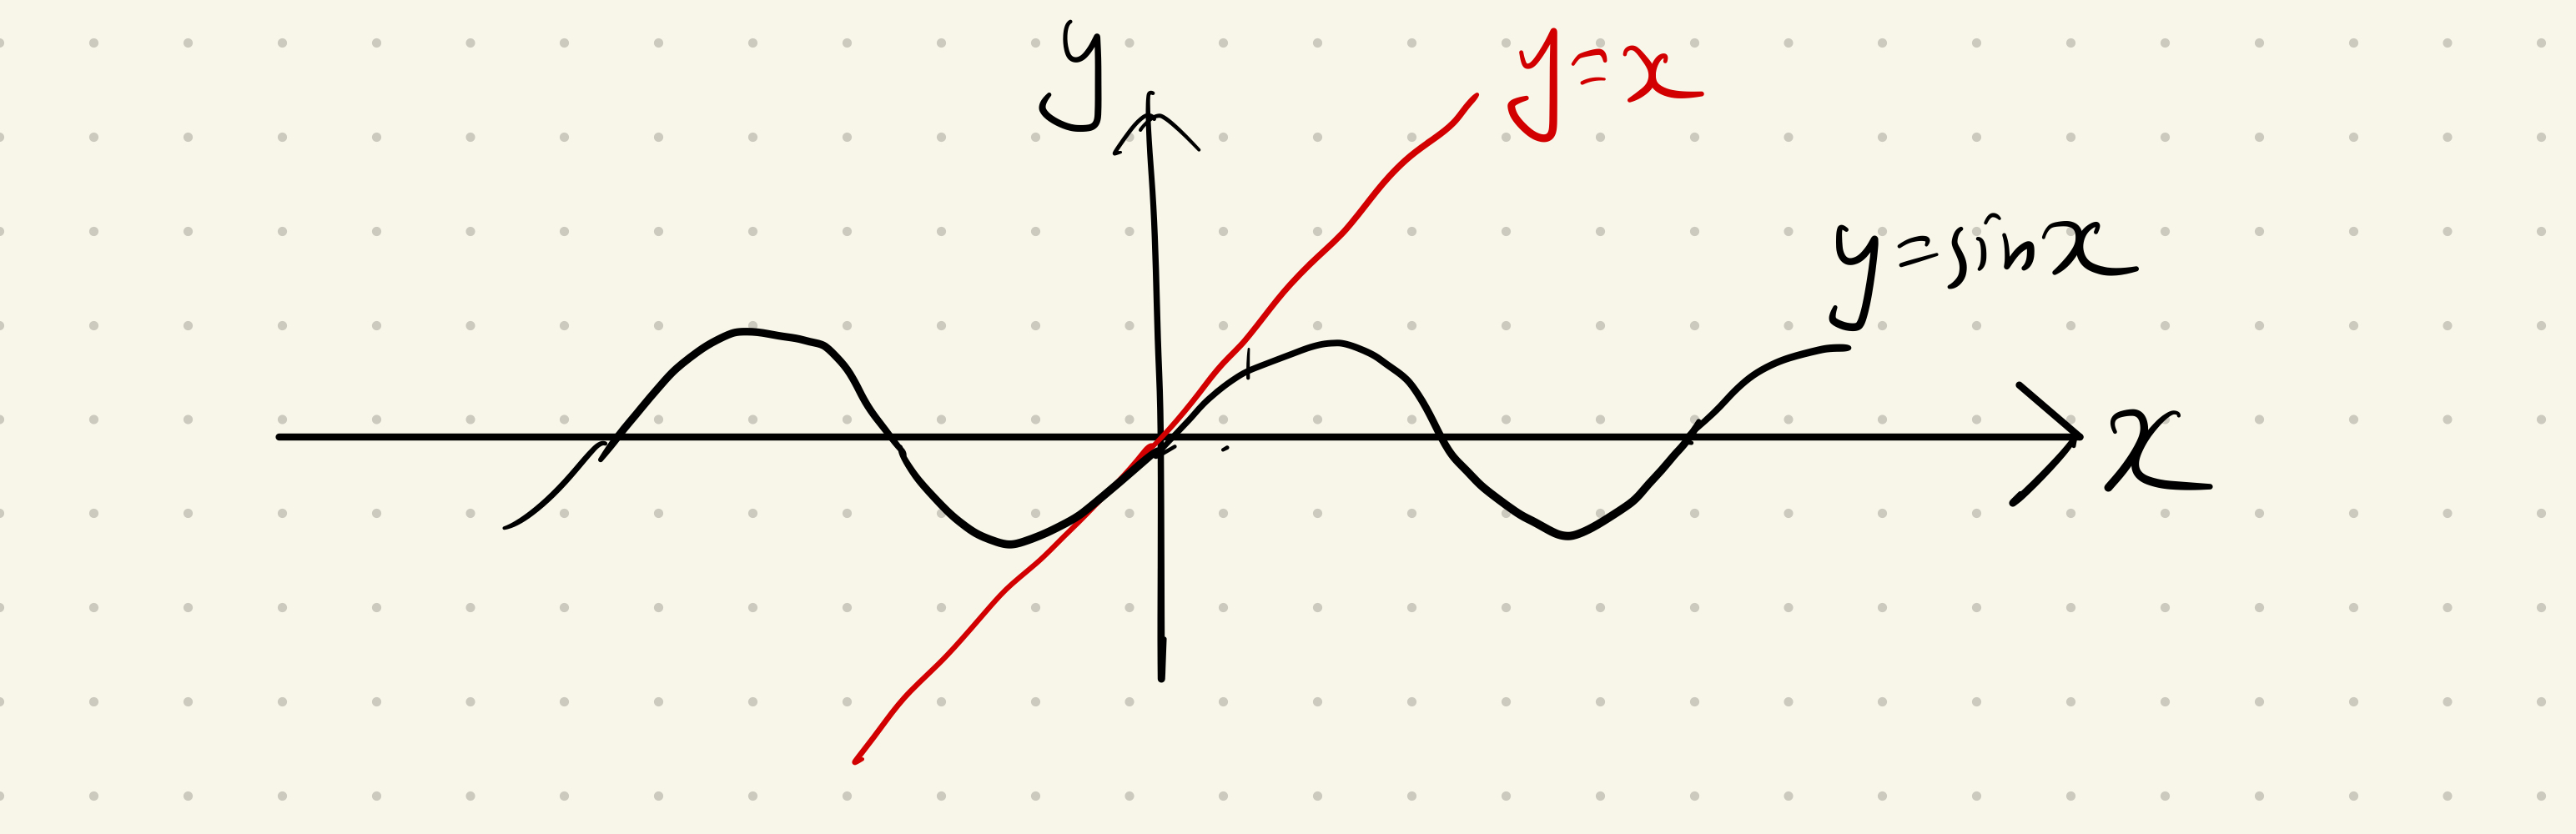
\includegraphics[width = 0.7\textwidth]{figures/chap 05/lin_approx_sin.png}
    \label{fig: lin_approx_sin}
\end{figure}

\begin{remark}
    The approximant for $\cos x$ seems weird: there is no $x$ in the approximant!  This indicates that when restricting to linear approximation, the behavior of $\cos x$ near $x=0$ is best approximated with a horizontal line, as shown in the graph:
\end{remark}

\begin{figure}[ht]
    \centering
    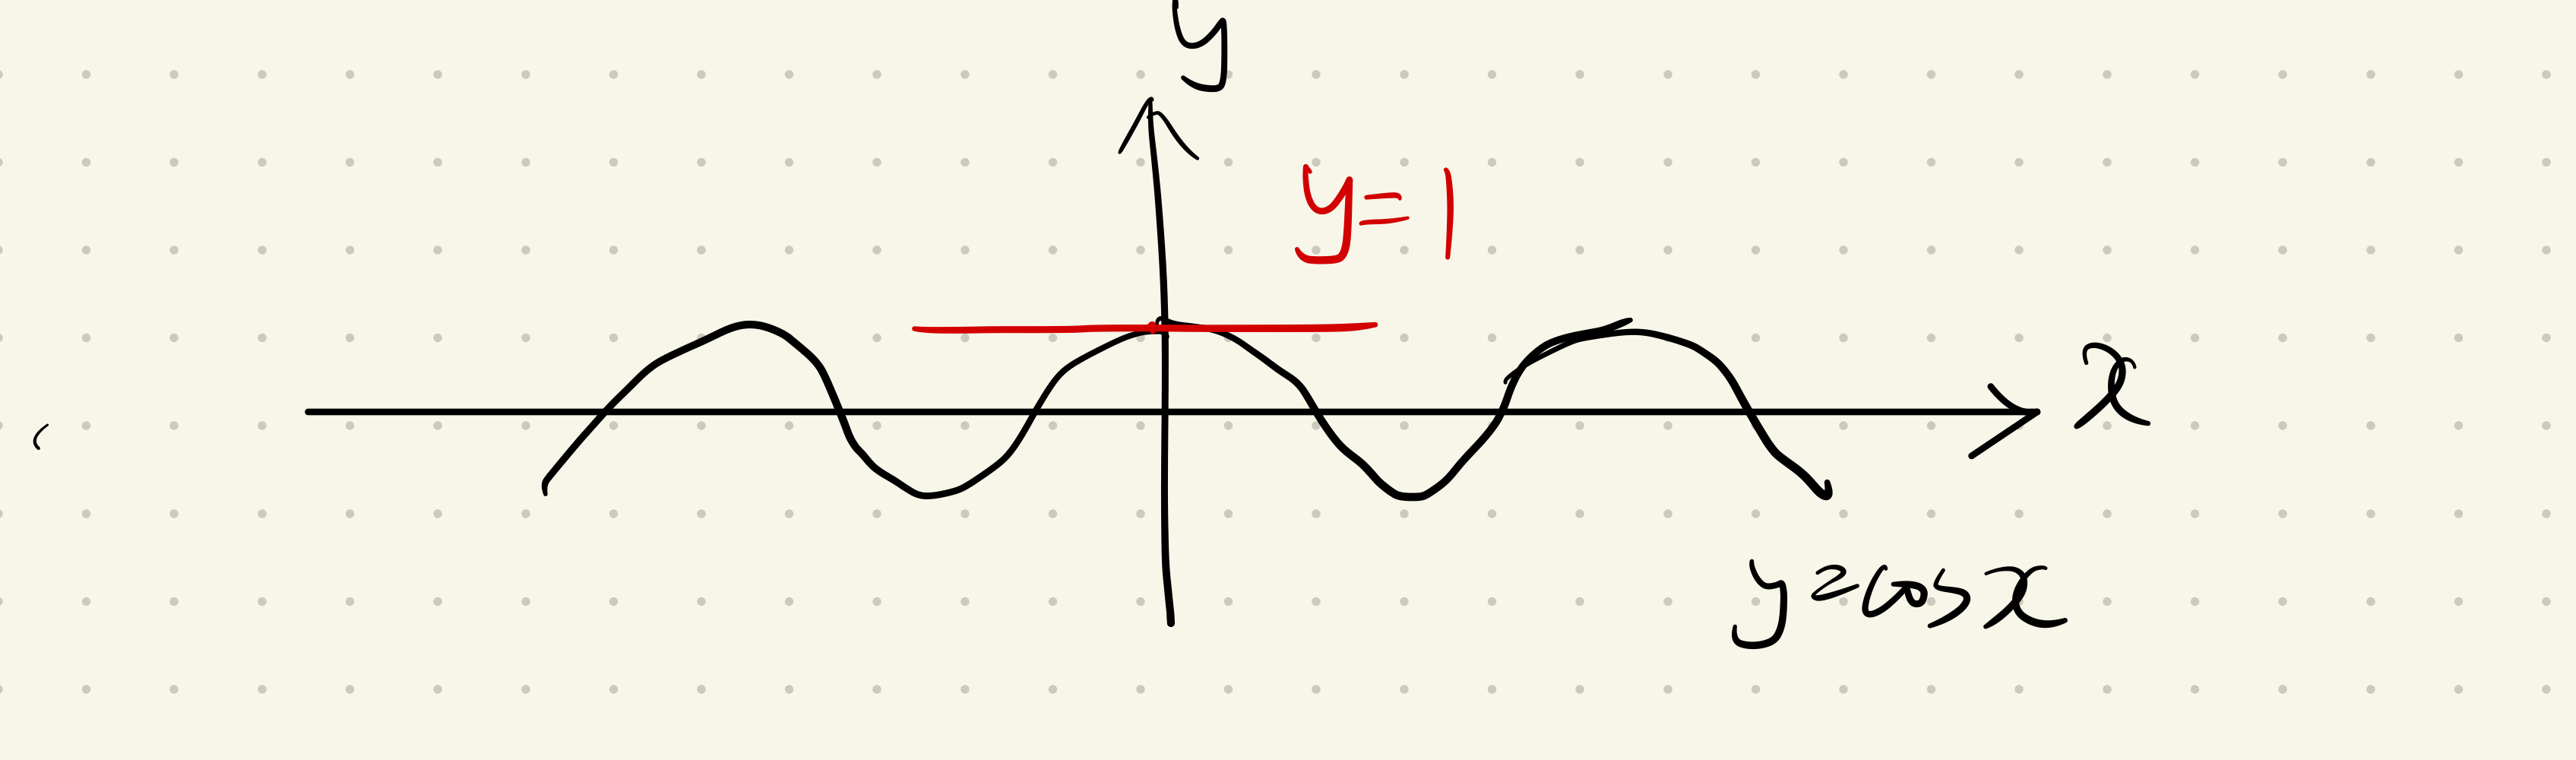
\includegraphics[width = 0.7\textwidth]{figures/chap 05/lin_approx_cos.png}
    \label{fig: lin_approx_cos}
\end{figure}

When functions are added / subtracted / multiplied with each other, we can do approximations to the individual functions first, then perform teh addtition / subtraction / multiplication.  We will demonstrate this in the following example.

\begin{eg}[]{eg: lin_approx_comb}
    Find the linear approximant to $f(x) = \frac{2e^x + \ln(1+x)}{\sqrt{1+x}}$ at $x = 0$.
\end{eg}

\begin{egsol}[]{egsol: lin_approx_comb}
    If we try to approximate $f(x)$ at $x=0$ with the tangent line formula, we first need to find its derivative with the quotient rule:
    \[f'(x) = \frac{\big(2e^x + \frac{1}{1+x}\big)\sqrt{1+x} - [2e^x + \ln(1+x)]\frac{1}{\sqrt{1+x}}}{\big(\sqrt{1+x}\big)^2}\]
    Therefore we have
    \[f(0) = \frac{2+0}{\sqrt{1}} = 2\]
    \[f'(0) = \frac{(2+1)\sqrt{1+0}-[2+0]\frac{1}{2\sqrt{1}}}{\big(\sqrt{1+0}\big)^2} = \frac{3-1}{1} = 2\]
    And the approximant is 
    \[\hat{f}(x) = f(0) + f'(0)(x-0) = 2+2x\]
    Alternatively, we can approximate first and get
    \begin{align*}
        f(x) &= [2e^x + \ln(1+x)](1+x)^{-\frac{1}{2}}\\
        &\approx [2(1+x) + x]\Big(1-\frac{1}{2}x\Big)\\
        &=[2+3x]\Big(1-\frac{1}{2}x\Big)\\
        &=2+2x-\frac{3}{2}x^2 \approx 2+2x
    \end{align*}
    The last approximation discards the $x^2$ term since when $x$ is near $0$, $x^2$ is negligible compared to $x$.  We can see that these two approaches yield identical results.
\end{egsol}

We will conclude linear approximations with an exercise:

\begin{ex}[]{ex: lin_approx_comb}
    Find the linear approximant to $f(x) = 3xe^{2x-10}$ at $x = 5$.
\end{ex}

\begin{exsol}[]{exsol: lin_approx_comb}
    (Approach 1) 
    
    We use the tangent line formula directly, so we first obtain the derivative of $f(x)$ 
    \[f'(x) = 3e^{2x-10} + 3xe^{2x-10}\cdot 2 = (6x+3)e^{2x-10}\]
    Therefore,
    \[f(5) = 3 \cdot 5 \cdot e^0 = 15\]
    \[f'(5) = (6 \cdot 5+3)e^0 = 33\]
    And the linear approximant is
    \[\hat{f}(x) = f(5) + f'(5)(x-5) = 15 + 33(x-5) = 33x-150\]
    
    (Approach 2)
    
    Let $x = 5 + \delta$, then when $x \approx 5$, $\delta \approx 0$, and we have
    
    \begin{align*}
        f(x) &= 3(5+\delta)e^{2(5+\delta)-10}\\
        &=3(5+\delta)e^{2\delta}\\
        &\approx3(5+\delta)(1+2\delta)\\
        &=15+33\delta+6\delta^2\\
        &\approx 15+33\delta = 15+33(x-5) = 33x-150
    \end{align*}
    
    The two approaches still yield the same linear approximant.
\end{exsol}

\subsection{Quadratic Approximation and Beyond}
Previously we used linear approximation to approximate $\cos x$ near $x=0$ and got $\cos x \approx 1$, which is somewhat anticlimactic.

\begin{figure}[ht]
    \centering
    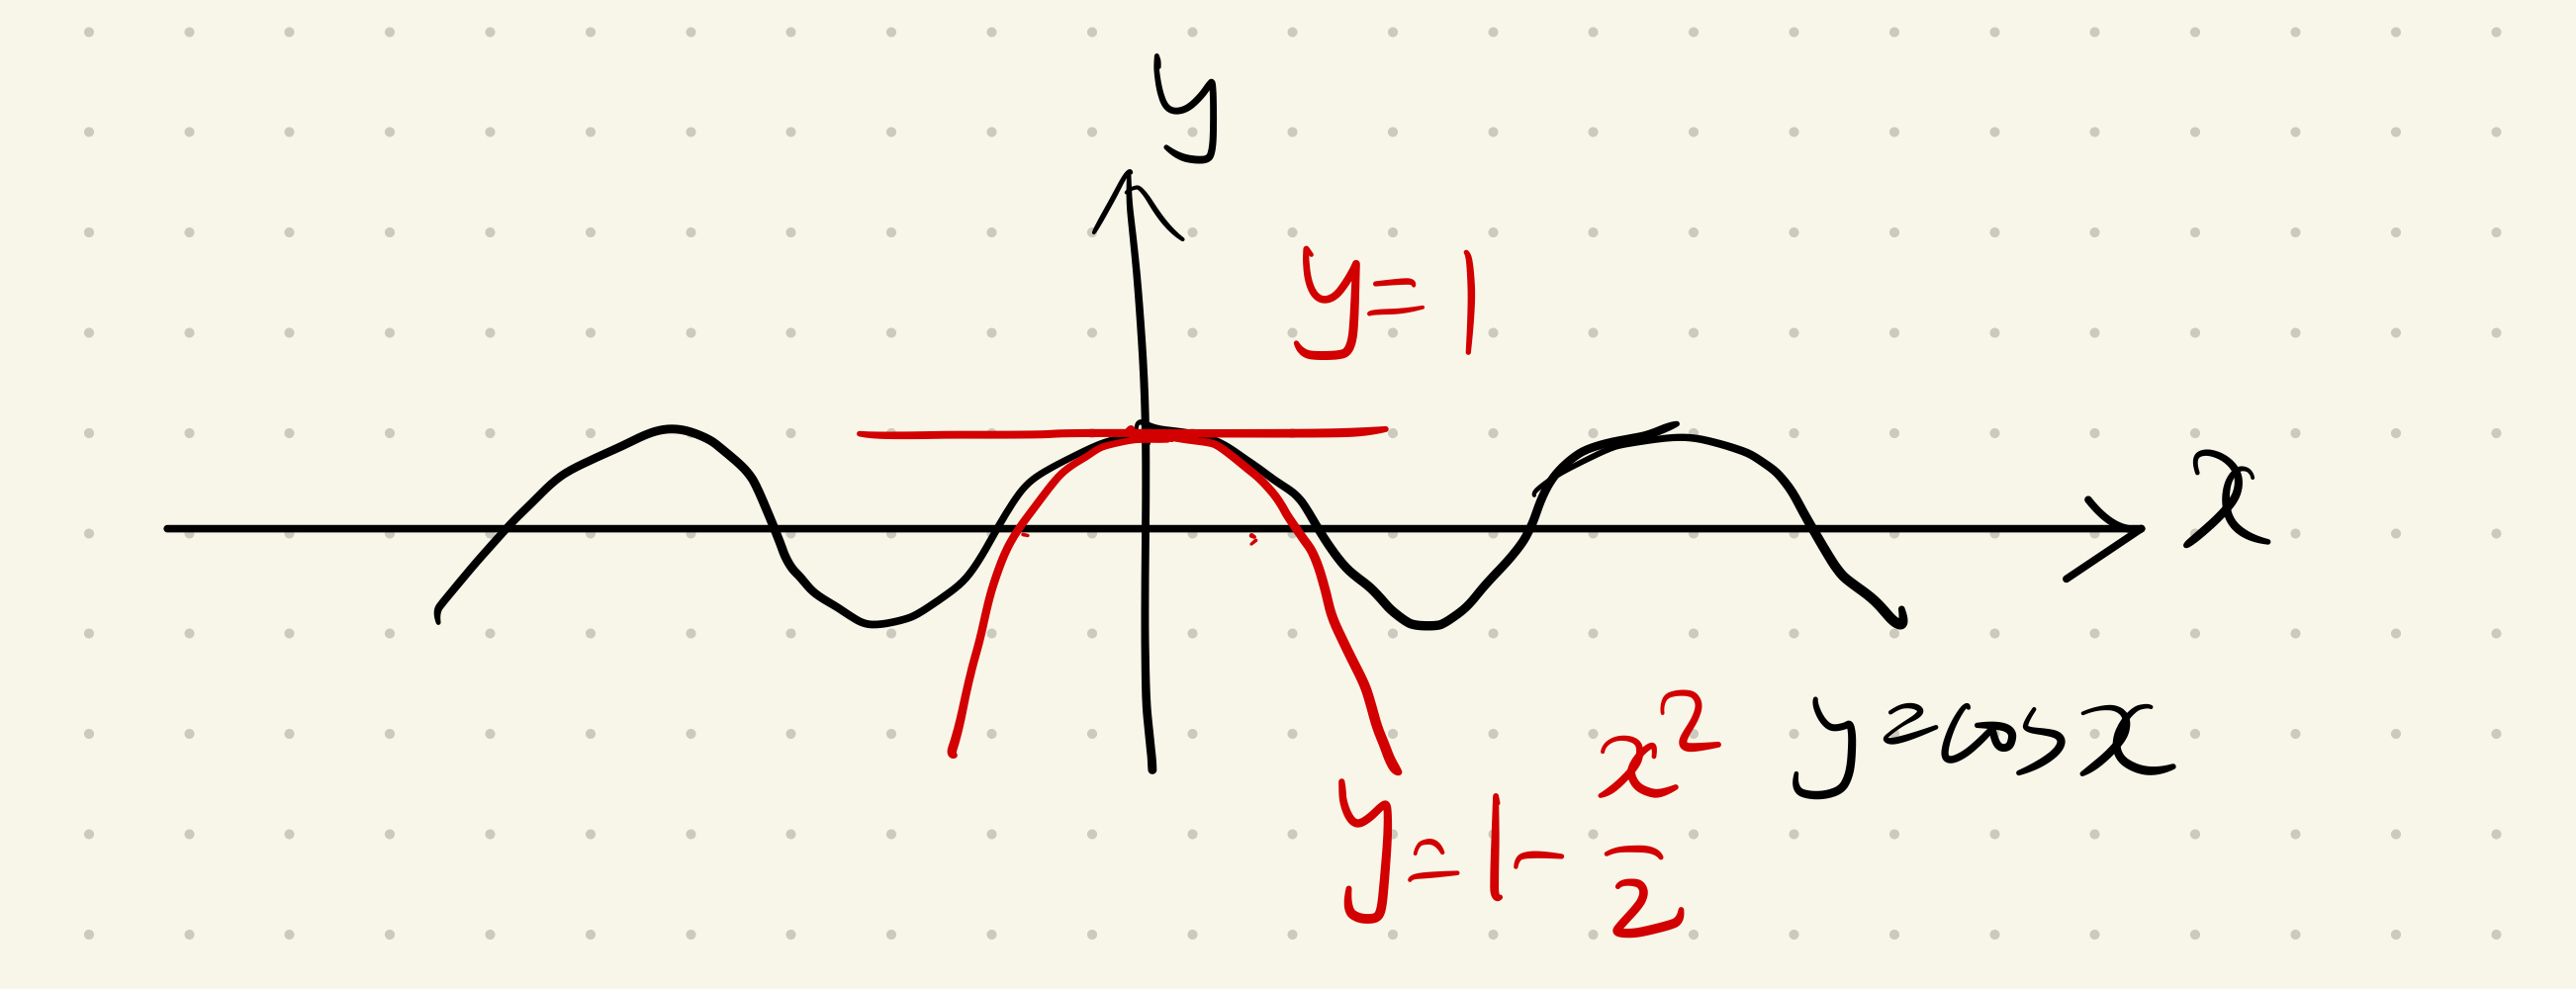
\includegraphics[width = 0.7\textwidth]{figures/chap 05/qua_approx_cos.png}
    \label{fig: qua_approx_cos}
\end{figure}

As shown in the graph above, although $y=1$ is the best line that approximates the behavior of $\cos x$ near zero, it is not doing a good job when $x$ is a bit far from zero.  A possible improvement is to use a degree-$2$ polynomial (parabola) instead of a degree-$1$ polynomial (line) to do the approximation, so that the approximant can curve and fit $\cos x$ better.

Suppose we want to approximate our desired function $f(x)$ near $x=a$.  Before we get to degree-$2$ polynomials, we first observe that if we write the degree-$1$ polynomial approximant as $\hat{f}_1(x) = b_0 + b_1(x-a)$, then matching the function value and derivative at $x=a$, i.e. letting $f(a) = \hat{f}_1(a)$ and $f'(a) = \hat{f}'_1(a)$, will give us the best solution $f(a) + f'(a)(x-a)$, as shown in the following table:

\begin{table}[ht]
    \centering
    \begin{tabular}{cccc}
        &Original function & Linear approximant & Quadratic approximant \\
        &$f(x)$ & $\hat{f}_1(x) = b_0+b_1(x-a)$ &  $\hat{f}_2(x) = b_0+b_1(x-a)+b_2(x-a)^2$ \\
        \hline
        Value @ $x=a$ & $f(a)$ & $b_0$ & $b_0$\\
        Derivative @ $x=a$ & $f'(a)$ & $b_1$ & $b_1$\\
        $2^{nd}$ derivative @ $x=a$ & $f''(a)$ & $0$ & $2b_2$
    \end{tabular}
    \label{tab: qua_approx}
\end{table}

Likewise, if we write the degree-$2$ polynomial approximant as $\hat{f}_2(x) = b_0 + b_1(x-a) + b_2(x-a)^2$, we can find the best solution by letting $f(a) = \hat{f}_2(a)$, $f'(a) = \hat{f}'_2(a)$ and $f''(a) = \hat{f}''_2(a)$. This leads to $b_0 = f(a)$, $b_1 = f'(a)$ and $b_2 = \frac{1}{2}f''(a)$, and we have the following theorem:

\begin{theo}[Quadratic approximation of general function]{thm: qua_approx}
    Suppose $f(x)$ is twice differentiable at $x=a$, then the best quadratic approximant for $f(x)$ at $x=a$ is 
    \[\hat{f}(x) = f(a)+f'(a)(x-a)+\frac{1}{2}f''(a)(x-a)^2\]
\end{theo}

We can then list some quadratic approximants for common functions:

\begin{table}[ht]
    \centering
    \begin{tabular}{ccccccc}
        $f(x)$ & $f'(x)$ & $f''(x)$ & $f(0)$ & $f'(0)$ & $f''(0)$ &$\hat{f}(x)$\\
        \hline
        $(1+x)^r$ & $r(1+x)^{r-1}$ & $r(r-1)(1+x)^{r-2}$ & $1$ & $r$ & $r(r-1)$ & $1+rx+\frac{r(r-1)}{2}x^2$ \\
        $e^x$ & $e^x$ & $e^x$ & $1$ & $1$ & $1$ & $1+x+\frac{1}{2}x^2$ \\
        $\ln(1+x)$ & $\frac{1}{1+x}$ & $-\frac{1}{(1+x)^2}$ & $0$ & $1$ & $-1$ & $x-\frac{1}{2}x^2$ \\
        $\sin x$ & $\cos x$ & $-\sin x$ & $0$ & $1$ & $0$ & $x$\\
        $\cos x$ & $-\sin x$ & $-\cos x$ & $1$ & $0$ &$-1$ & $1-\frac{1}{2}x^2$
    \end{tabular}
    \label{tab: qua_approx_deriv}
\end{table}

We summarize the results into the following theorem:

\begin{theo}[Quadratic approximation of common functions]{thm: qua_approx_fxn}
    When $x \approx 0$, we have the following quadratic approximations:
    \[(1+x)^r \approx 1+rx+\frac{r(r-1)}{2}x^2 \qquad e^x \approx 1+x+\frac{x^2}{2} \qquad \ln(1+x) \approx x-\frac{x^2}{2}\]
    \[\sin x \approx x \qquad \cos x \approx 1-\frac{x^2}{2} \]
\end{theo}

\begin{remark}
    Notice that our quadratic approximant for $\cos x$ near $x=0$ performs much better than the linear approximant, especially when $x$ is a bit away from $0$, as shown in the graph above.  Also, the quadratic approximant for $\sin x$ near $x=0$ is the same as its linear approximant, which implies that introducing an extra $x^2$ term does not improve the approximation of $\sin x$ near $x=0$.
\end{remark}

In fact, by the virtue of linear and quadratic approximants, if we try to approximate $f(x)$ near $x=c$ with higher order polynomials by matching an array of high-order derivatives at $x=c$, eventually we will get the famous \textit{Taylor series}:

\[\sum_{n=0}^\infty\frac{f^{(n)}(a)}{n!}(x-a)^n = f(a) + f'(a)(x-a) + \frac{f''(a)}{2!}(x-a)^2 + \frac{f'''(a)}{3!}(x-a)^3 + \cdots\]

Under certain conditions (which we will not dig further into for now), this series is actually an accurate representation for $f(x)$.  In other words, it is no longer an approximation to $f(x)$: it \textit{is} $f(x)$.  We provide some of the famous Taylor series below:

\begin{theo}[Taylor series of common functions]{thm: taylor_fxn}
    \vspace{-0.5cm}
    \begin{align*}
        e^x &= 1 + x + \frac{x^2}{2!} + \frac{x^3}{3!} + \frac{x^4}{4!} + \cdots\\
        \sin x &= x - \frac{x^3}{3!} + \frac{x^5}{5!} - \frac{x^7}{7!} + \cdots\\
        \cos x &= 1 - \frac{x^2}{2!} + \frac{x^4}{4!} - \frac{x^6}{6!} + \cdots\\
        \ln(1+x) &= x - \frac{x^2}{2} + \frac{x^3}{3} - \frac{x^4}{4!} + \cdots \qquad (-1 < x \le 1)\\
        \frac{1}{1-x} &= 1 + x + x^2 + x^3 + x^4 + \cdots \qquad (-1 < x < 1)
    \end{align*}
\end{theo}

To digress a little bit, although in this course we only talk about real numbers, but if we define $i = \sqrt{-1}$ as the imaginary square root of $-1$ and plug $ix$ into the Taylor series for $e^x$, we get

\begin{align*}
    e^{ix} &= 1+ix+\frac{(ix)^2}{2!} + \frac{(ix)^3}{3!} + \frac{(ix)^4}{4!} + \frac{(ix)^5}{5!} + \frac{(ix)^6}{6!} - \frac{(ix)^7}{7!} + \cdots \\
    &= 1+ix-\frac{x^2}{2!} - \frac{ix^3}{3!} + \frac{x^4}{4!} + \frac{ix^5}{5!} - \frac{x^6}{6!} + \frac{ix^7}{7!} + \cdots \\
    &= \left(1 - \frac{x^2}{2!} + \frac{x^4}{4!} - \frac{x^6}{6!} + \cdots\right) + i\left(x - \frac{x^3}{3!} + \frac{x^5}{5!} - \frac{x^7}{7!} + \cdots\right)\\
    &= \cos x + i \sin x
\end{align*}

which is a remarkable result proposed (popularized) by the famous mathematician \textit{Leonhard Euler} (1707-1783).  In addition, pluggin $\pi$ into $x$ and we yield $e^{i\pi} = -1$. Or, even better,
\[e^{i\pi}+1 = 0\]
This formula, also termed as \textit{Euler's identity}, is considered as the most beautiful formula by some, since it relates five of the fundamental numbers in mathematics: $e$, $\pi$, $i$, $1$, $0$, all in a compact and simple formula.
\newpage

\section{Newton's Method}
Derivatives are also useful in finding roots of a function $f(x)$, i.e. finding $x$ where $f(x) = 0$.  Sometimes you \textit{can} find the roots by simply solving $f(x)=0$ on paper, but for complicated functions (eg. $f(x) = x^2 - \sin x$) you have to resort to numerical methods, which approximate the roots using iterative procedures.  Newton's method is one of the numerical methods that has a fairly fast speed of convergence (i.e. it can get you a pretty accurate answer within a few iterations).

For example, suppose we want to find the roots of $f(x) = x^2-3$.  In this case, we know its roots are $\pm \sqrt{3}$ by solving $x^2-3 = 0$, but we now try to find the roots numerically.  To initiate Newton's method, we must first guess a solution that is not too far off.  We notice $f(1) = -2 < 0$ and $f(2) = 1 > 0$, so there is (probably) a root between $1$ and $2$.  Let's make a initial guess of $1$.  Since this is our initial guess, we denote it as $x_0 = 1$.  This gives us a graph a follows:

\begin{figure}[ht]
    \centering
    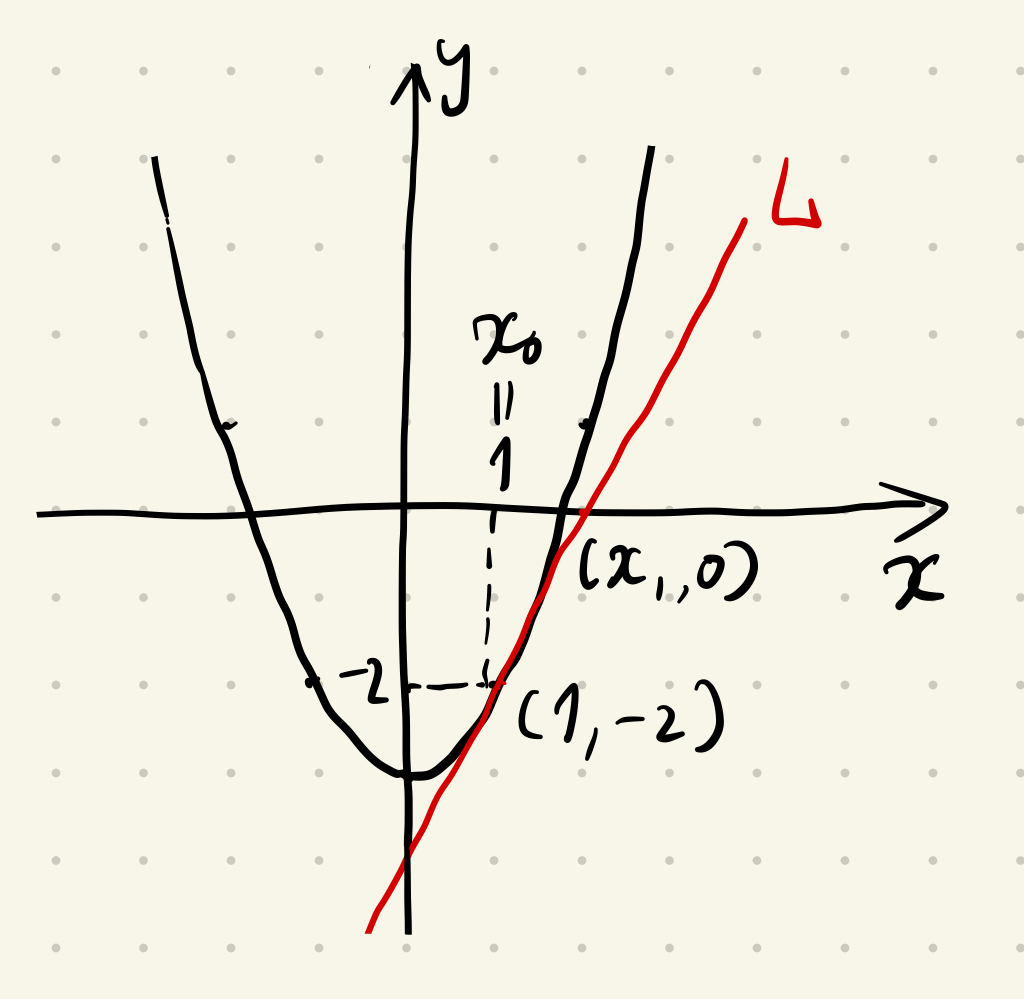
\includegraphics[width = 0.5\textwidth]{figures/chap 05/newton_1.png}
    \label{fig: newton_1}
\end{figure}

We see that our guess of $x_0 = 1$ is not quite correct since $f(x_0) = -2$.  However, from this point on the curve we can construct a tangent line $L$ that intersects with the $x$-axis at $(x_1, 0)$.  The mindset is that if $L$ is a good linear approximation to $f(x)$ near $x = 1$, then $(x_1, 0)$ should be very close to the point where the curve intersects the $x$-axis.  Knowing that $f'(x) = 2x$, we can express $L$ using our tangent line formula (or linear approximation formula, if you will):
\[L: y = -2 + 2(x-1) = 2x-4\]
Since $L$ passes through $(x_1, 0)$, the following equation should be satisfied: 
\[0 = 2x_1-4\]
So we get our next guess $x_1 = 2$, which still isn't quite right since $f(2) = 1$.  We can apply the same trick again, i.e. do another iteration of Newton's method based on the following graph (which is scaled and a little distorted for demonstration):

\begin{figure}[ht]
    \centering
    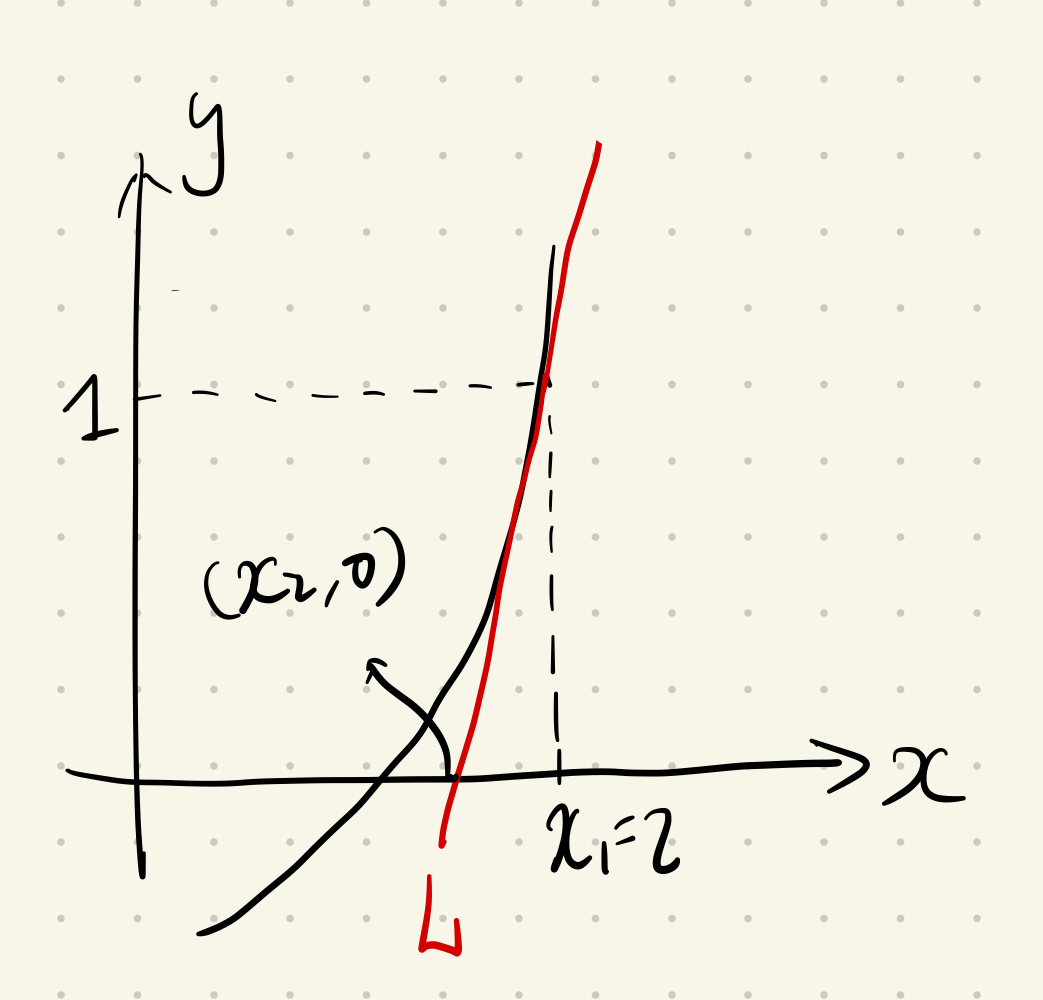
\includegraphics[width = 0.5\textwidth]{figures/chap 05/newton_2.png}
    \label{fig: newton_2}
\end{figure}

The equation for the new tangent line, which passes through $(2, f(2) = 1)$, is
\[L: y = 1 + 4(x-2) = 4x-7\]
using the fact that $f'(2) = 2 \cdot 2 = 4$.  Following the same procedure, we aim to find the point where $L$ intersects with the $x$-axis, $(x_2, 0)$.  Since $L$ passes through $(x_2, 0)$, we have
\[0 = 4x_2-7\]
So we have our next guess $x_2 = \frac{7}{4}$.  Now you can see that $f\big(\frac{7}{4}\big) = 0.0625$, which is really close to $0$, so we're very close to our solution.  In practice, we can set a small positive number $\epsilon$ (sometimes termed as \textit{tolerance}) that stands for the maximum error magnitude in function value we are willing to accept, then repeat the iterations until $|f(x_k)| < \epsilon$ and claim $x_k$ is our approximated root and call it a day.  If we set the tolerance as $10^{-8}$, then we only need $4$ iterations to arrive at our answer:

\begin{table}[ht]
    \centering
    \begin{tabular}{cccc}
        Iteration number & Root estimate & Error in function value & Error of estimate\\
        ($k$) & ($x_k$) & ($f(x_k)$) & ($x_k - \sqrt{3}$)\\
        \hline
        $0$ & $1$ & $-2$ & $-0.7321$\\
        $1$ & $2$ & $1$ & $0.2679$\\
        $2$ & $7/4$ & $0.0625$ &  $0.0179$\\
        $3$ & $97/56$ & $3.19\times 10^{-4}$ & $9.20 \times 10^{-5}$\\
        $4$ & $18817/10864$ & $8.47\times 10^{-9}$ & $2.45 \times 10^{-9}$
    \end{tabular}
    \label{tab: newton_iteration}
\end{table}

\begin{remark}
    The iteration is actually going closer and closer to one of the roots, $\sqrt{3}$, but does not get anywhere near the other root, $-\sqrt{3}$.  To find the other root, we will have to pick an initial value closer to $-\sqrt{3}$, eg. $x_0 = -1$.
\end{remark}

Note that although Newton's methods is quite powerful, in some cases it will fail miserably.  One of the failure modes is when Newton's method iterates to a point where the derivative is zero.  For example, if we make our initial guess of $x_0 = 0$, then $f'(x_0) = 0$, so the tangent line $L$ is horizontal and does not intersect with the $x$-axis and we do not know how to make the next guess $x_1$. 

Another failure mode of Newton's method is when the root estimate jumps between several points and does not converge.  For example, in the following figure, if you initialize at $x = x_0$, the next guess would be $x = x_1$.  Yet in the next iteration, plugging in $x_1$ will lead you back to $x_0$, and you will get nowhere near the true root $x^*$.  The two failure modes mentioned above can be circumvented by choosing a better initial guess of $x_0$.  

\begin{figure}[ht]
    \centering
    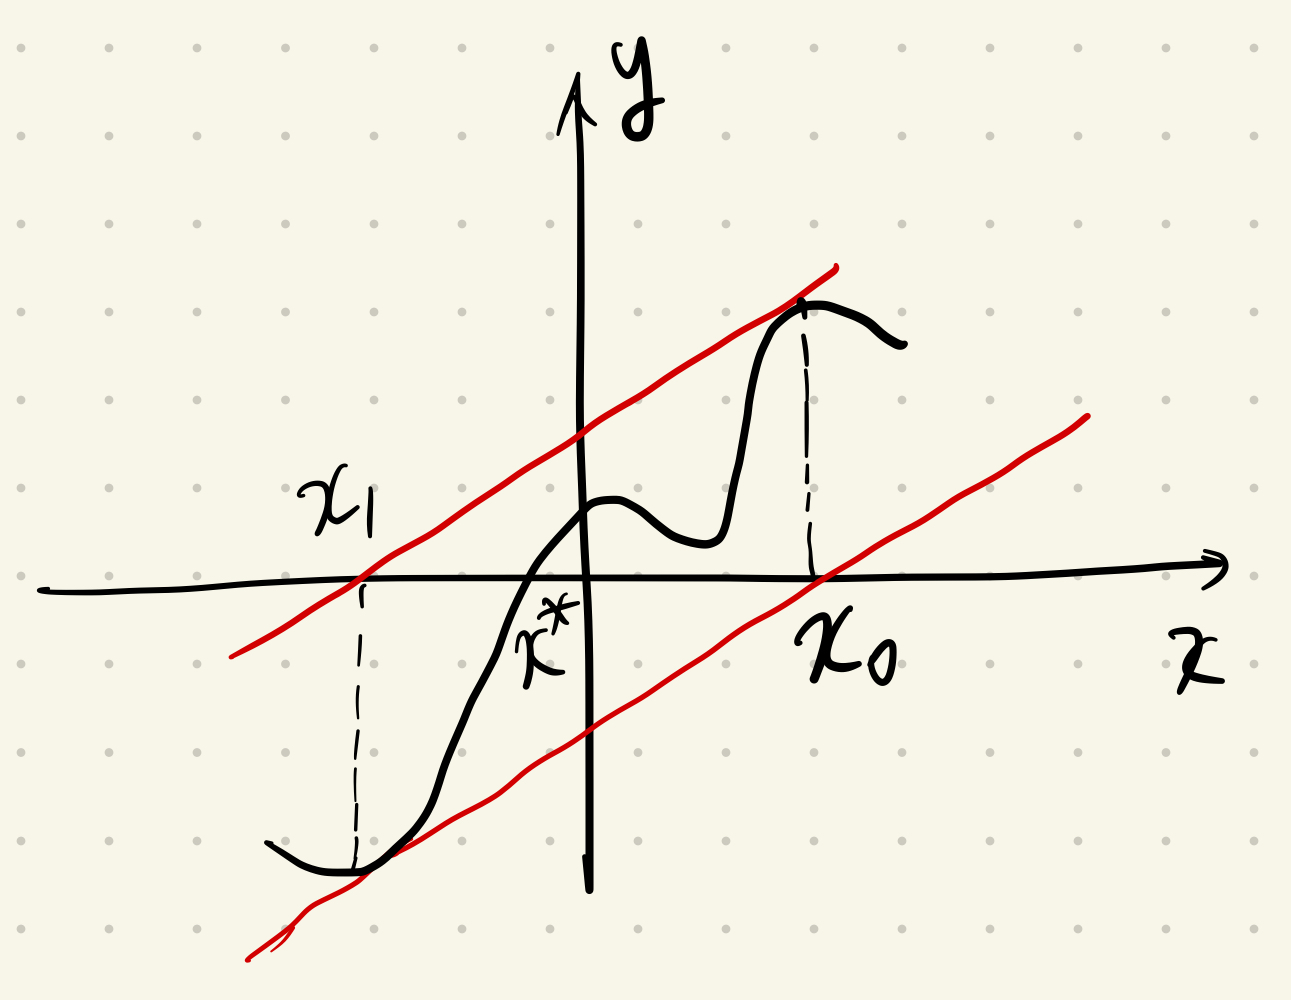
\includegraphics[width = 0.5\textwidth]{figures/chap 05/newton_3.png}
    \label{fig: newton_3}
\end{figure}

There are still other failures modes for Newton's method, but we will not discuss further: just keep in mind that if Newton's method is taking a lot of iterations and does not seem to be converging, you may have encountered a case where Newton's method fails.  You should try changing your initial guess or opting for another root-finding algorithm.

Lastly, we derive the general formula for each iteration of Newton's method.  Suppose we are finding the roots of $f(x)$, and our current guess is $x_k$, the tangent line over $(x_k, f(x_k))$ is:
\[L: y = f(x_k) + f'(x_k)(x-x_k)\]
The next guess for the root, $x_{k+1}$, is the $x$-coordinate of intersection point between $L$ and the $x$-axis, i.e. $L$ passes through $(x_{k+1}, 0)$.  So we have
\[0 = f(x_k) + f'(x_k)(x_{k+1}-x_k)\]
Rearrange the equation and we get the following theorem:

\newpage

\begin{theo}[Iteration formula for Newton's method]{thm: newton}
    Let $x_k$ be root estimate for $f(x)$ from the $k^{\text{th}}$ iteration in Newton's method, then the root estimate of the next iteration, $x_{k+1}$, can be found by
    \[x_{k+1} = x_k - \frac{f(x_k)}{f'(x_k)}\]
\end{theo}

From this formula, you can see that the failure mode where the derivative is zero becomes evident, since zero would then be in the denominator and the procedure does not make sense.  We will end this section with an exercise.

\begin{ex}[]{ex: newton}
    Approximate the value of $\sqrt[3]{2}$ by finding the root of $f(x) = x^3 - 2$ with Newton's method.
\end{ex}

\begin{exsol}[]{exsol: newton}
    First, we obtain the derivative of $f(x)$, which is $f'(x) = 3x^2$.  The iteration formula is then
    
    \[x_{k+1} = x_k-\frac{x_k^3-2}{3x_k^2}\]
    
    Now we must make an initial guess, $x_0$, for the root of $f(x)$.  Since we know that $f(1) = -1 < 0$ and $f(2) = 6 > 0$, we reckon that there should be a root for $f(x)$ between $1$ and $2$, and we set $x_0 = 1$ for convenience.  We also set the tolerance $\epsilon$ to be $10^{-4}$.
    
    \vspace{0.3cm}
    
    \begin{center}
        \begin{tabular}{ccc}
            Iteration number & Root estimate & Error in function value\\
            $(k)$ & $\Big(x_k = x_{k-1}-\frac{x_{k-1}^3-2}{3x_{k-1}^2}\Big)$ & $(x_k^3-2)$\\
            \hline
            $0$ & $1$ & $-1$\\
            $1$ & $4/3$ & $0.370$\\
            $2$ & $91/72$ & $0.0190$\\
            $3$ & $1126819/894348$ & $5.93\times 10^{-5}$
        \end{tabular}
    \end{center}
    
    We thus have our estimate $x_3 = \frac{1126819}{894348} \approx 1.2599335$.  
    
    Compared to the true root $\sqrt[3]{2} \approx 1.2599210$, we are accurate to the fourth decimal.  Actually, if we lower our tolerance and allow one more iteration, we can be accurate to the seventh decimal.
    \label{tab: newton_iteration_ex}
\end{exsol}

\newpage
\section{Related Rates}
In some application problems, we known the relationship between two or more variables, eg. price and demand of a product; volume, surface area and radius of a ball.  Since these variables are inter-related, if one variable is changing with time at a certain rate, the other variables will also be changing with time based on the given relationship, and its rate of change can be deduced using derivatives.  In these types of problems, implicit differentiation will come in handy frequently.  To see this, let us look at the following examples:

\begin{eg}[]{eg: related_rates_balloon}
    An air nozzle is blowing air into the balloon at the speed of $150\text{ cm}^3/\text{sec}$. Suppose we can treat the balloon as a perfect sphere and the balloon is now $10$ cm in diameter.  How fast is the diameter of the balloon growing right now? 
\end{eg}

\begin{egsol}[]{egsol: related_rates_balloon}
    If we denote the diameter of the balloon as $D$ (cm) and its volume as $V$ (cm$^3$), then we can relate them with the following equation:
    \[V =\frac{4}{3}\pi \Big(\frac{D}{2}\Big)^3 = \frac{\pi}{6}D^3\]
    To obtain the related rates between $V$ and $D$, we differentiate both sides of the equation by time $t$ (measured in seconds).  Note that $V$ and $D$ are both functions of $t$, so we need to use the chain rule along the way:
    \begin{align*}
        \frac{d}{dt}V &= \frac{d}{dt}\Big(\frac{\pi}{6} D^3\Big)\\
        \frac{dV}{dt} &= \frac{\pi}{6}\frac{dD^3}{dt} = \frac{\pi}{6}\frac{dD^3}{dD}\frac{dD}{dt} = \frac{\pi}{6}\cdot 3D^2 \frac{dD}{dt} = \frac{\pi}{2} D^2 \frac{dD}{dt}
    \end{align*}
    Or we may use the Lagrange notation, defining $()'$ as differentiating with respect to $t$:
    \[V' = \Big(\frac{\pi}{6} D^3\Big)' = \frac{\pi}{6}(D^3)' = \frac{\pi}{6}\cdot 3D^2 \cdot D' = \frac{\pi}{2} D^2D'\]
    Since the nozzle is blow air at the speed of $150\text{cm}^3/\text{sec}$ and the balloon is currently $10$cm in diameter, we have $V' = 150$ and $D = 10$, so 
    \[150 = \frac{\pi}{2}10^2 D' \quad \Rightarrow \quad D' = \frac{3}{\pi}\] 
    which implies the diameter of the balloon is growing at $\frac{3}{\pi}$cm/sec.
\end{egsol}

\begin{eg}[]{eg: related_rates_ladder}
    A $2.5$-meter ladder leaning against a wall is starting to slide off.  Suppose the foot of the ladder is moving away from the wall at the speed of $20$ cm/sec when it is $1.5$ meters away from the wall base.  How fast is the tip of the ladder sliding down against the wall now?
\end{eg}

\begin{egsol}[]{egsol: related_rates_ladder}
    Based on the description of the problem, we can draw a graph as follows:
    \begin{center}
        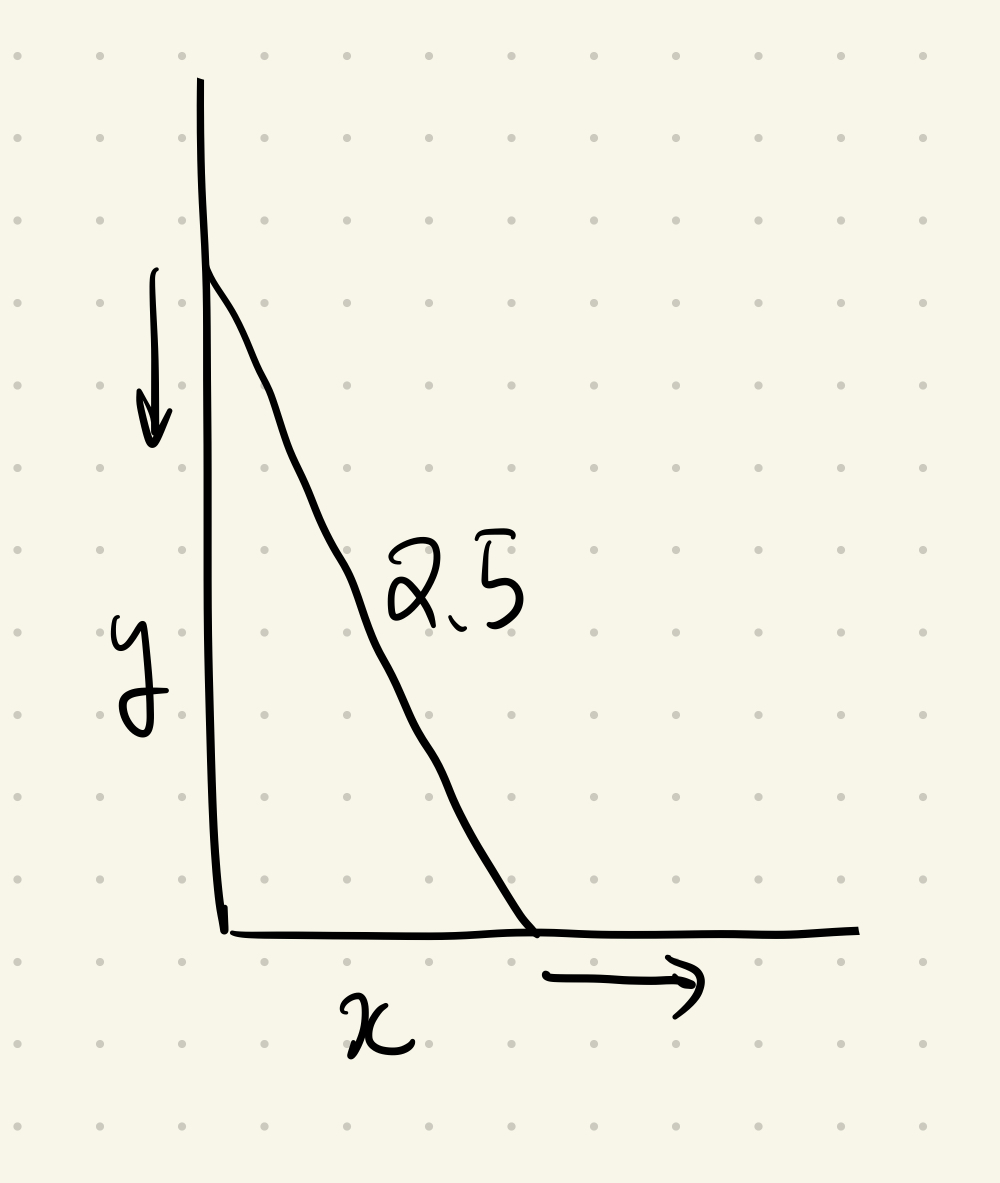
\includegraphics[width = 0.3\textwidth, trim={0 2cm 0 3cm}, clip]{figures/chap 05/rel_rates_ladder.png}
        \label{fig: rel_rates_ladder}    
    \end{center}
    where $x$ (in meters) is the distance between the ladder foot and the wall base, and $y$ (in meters) is the height of the ladder tip.  From Pythagorean theorem, we relate $x$ and $y$ by:
    \[x^2+y^2 = 2.5^2 = 6.25\]
    To obtain the related rates between $x$ and $y$, we differentiate both sides by $t$ (denoting $()'$ as differentiation with respect to $t$):
    \begin{align*}
        (x^2+y^2)' &= (6.25)'\\
        2xx'+2yy' &= 0\\
        y' &= -\frac{xx'}{y}  \quad  (\because y > 0)
    \end{align*}
    Since the foot of the ladder is moving \textit{away} from the wall with speed $0.2$m/sec, and it is currently $1.5$m away from the wall base, we have
    \[x' = 0.2 \qquad x = 1.5 \qquad y = \sqrt{2.5^2-1.5^2} = 2\]
    Therefore, 
    \[y' = -\frac{0.2 \cdot 1.5}{2} = -0.15\]
    So the tip of the ladder is sliding down with speed $15$cm/s. (The negative sign in $y'$ indicates that $y$ is decreasing, which reflects that the tip is sliding down.)
\end{egsol}

\begin{ex}[]{ex: related_rates_orbit}
    \begin{center}
        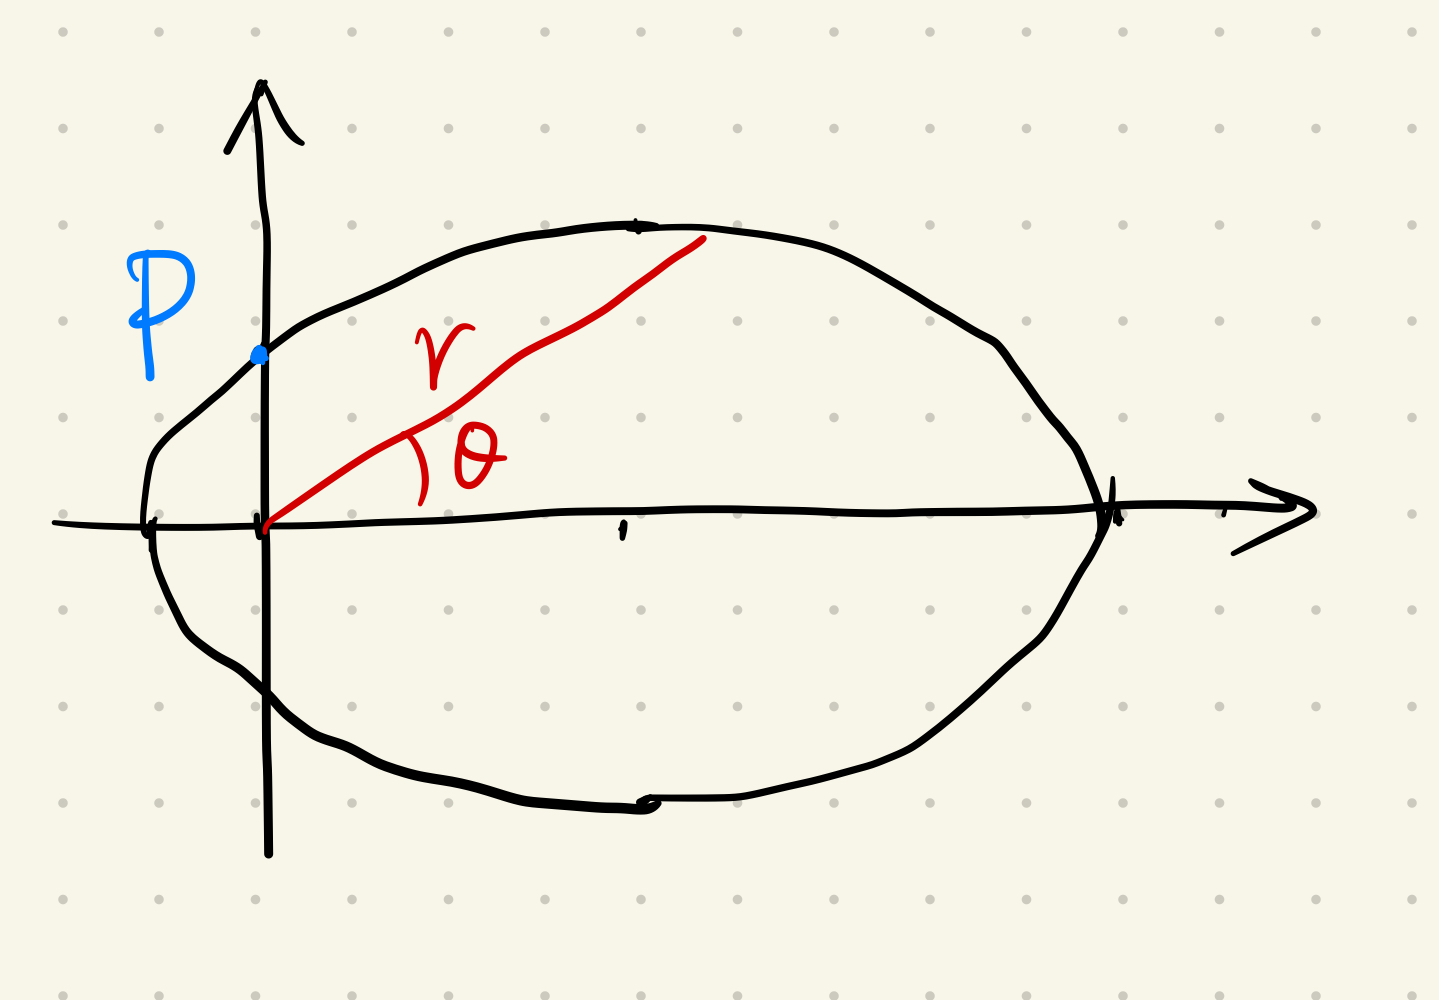
\includegraphics[width = 0.3\textwidth]{figures/chap 05/rel_rates_orbit.png}
        \label{fig: rel_rates_orbit}    
    \end{center}
    Shown in the figure above, a moon is orbiting counter-clockwise around a planet at the origin point.  The orbit, which is an ellipse, can be described as follows:
    %\[\frac{(r\cos \theta - 4)^2}{25} + \frac{(r \sin \theta)^2}{9} = 1\]
    \[r\Big(1-\frac{4}{5}\cos \theta \Big) = \frac{9}{5}\]
    where $r$ (in AU, astronomical unit) is the distance between the moon and the planet, and $\theta$ is the directed angle from the long axis of the ellipsis to the moon-planet line.  Suppose an astronomer observed that the angular velocity of the moon at point $P$ is $0.2$ radians/day, how fast is the moon-planet distance decreasing at that time?
\end{ex}

\begin{exsol}[]{exsol: related_rates_orbit}

    We try to find the related rate by differentiating both sides of the orbit equation by time $t$ (in days).  For brevity, we denote $()'$ as differentiation with respect to $t$:
    \begin{align*}
        % \left[\frac{(r\cos \theta - 4)^2}{25} + \frac{(r \sin \theta)^2}{9}\right]' &= (1)' = 0\\
        % \frac{\big[(r \cos \theta - 4)^2\big]'}{25} + \frac{\big[(r \sin \theta)^2\big]'}{9}&= 0\\
        % \frac{\big[(r \cos \theta - 4)^2\big]'}{25} &= -\frac{\big[(r \sin \theta)^2\big]'}{9}\\
        % \frac{2(r\cos \theta -4)(r\cos \theta -4)'}{25} &= - \frac{2(r\sin \theta) (r\sin\theta)'}{9}\\
        % \frac{(r\cos \theta -4)(r'\cos \theta -r(\sin \theta)\theta' )}{25} &= - \frac{(r\sin \theta) (r'\sin\theta + r (\cos \theta) \theta')}{9}
        \Big[r\Big(1-\frac{4}{5}\cos \theta \Big)\Big]' &= \Big(\frac{9}{5}\Big)'\\
        r'\Big(1-\frac{4}{5}\cos \theta \Big) + r\Big(1-\frac{4}{5}\cos \theta \Big)'&= 0\\
        r'\Big(1-\frac{4}{5}\cos \theta \Big) + r\Big(-\frac{4}{5} (-\sin \theta) \theta')'&= 0\\
        r'\Big(1-\frac{4}{5}\cos \theta \Big) + \frac{4}{5} r \theta' \sin \theta &= 0
    \end{align*}
    At point $P$, we have $\theta = \frac{\pi}{2}$ and $\theta' = 0.2$.  Plugging in $\theta = \frac{\pi}{2}$ into the orbit equation and we can solve for $r$ at point $P$:
    \[r = \frac{9}{5}\Big/\Big(1-\frac{4}{5}\cos \frac{\pi}{2} \Big) = \frac{9}{5}\]
    %\begin{align*}
        % \frac{(r\cos \frac{\pi}{2} - 4)^2}{25} + \frac{(r \sin \frac{\pi}{2})^2}{9} &= 1\\
        % \frac{16}{25} + \frac{r^2}{9} &= 1\\
        % r^2 &= \frac{81}{25}  \Rightarrow r = \frac{9}{5} \quad (\because r \ge 0)
    %\end{align*}
    We can then plug in $\theta = \frac{\pi}{2}$, $\theta' = 0.2$ and $r = \frac{9}{5}$ into the previous equation and yield
    \begin{align*}
        r'\Big(1-\frac{4}{5}\cos \frac{\pi}{2} \Big) + \frac{4}{5} \frac{9}{5} \cdot 0.2 \cdot \sin \frac{\pi}{2} &= 0\\
        r' + \frac{36}{125} &= 0 \quad \Rightarrow \quad r' = -\frac{36}{125} = -0.288
    \end{align*}
    Therefore, the moon-planet distance is decreasing at a rate of $0.288$ AU/day, where the negative sign we've got indicates that the distance is decreasing.
\end{exsol}

\begin{ex}[]{ex: related_rates_cars}
    Two cars $A$ and $B$ are driving away from town $O$. $A$ is driving straight to the east, while $B$ is driving toward the north-east, so that the routes of the two cars are $45\degree$ apart.  Suppose $A$ is $20$ km from town $O$ and driving at $60$ km/hr, and $B$ is $20\sqrt{2}$ km from town $O$ and driving at $100$ km/hr.  What is the rate of change for the distance between the two cars?
\end{ex}

\begin{exsol}[]{egsol: related_rates_car}
    Let the distance between $A$ and $O$ be $a$ (kilometers), between $B$ and $O$ be $b$ (kilometers), and distance between $A$ and $B$ be $c$ (kilometers).  From the Cosine Theorem, we have the relationship between $a$, $b$ and $c$ as:
    \[c^2 = a^2 + b^2 - 2ab\cos 45 \degree = a^2 + b^2 - \sqrt{2}ab\]
    We try to find the related rate by differentiating both sides by time $t$ (in seconds).  For brevity, we denote $()'$ as differentiation with respect to $t$:
    \begin{align*}
        (c^2)' &= (a^2 + b^2 - \sqrt{2}ab)'\\
        2cc' &= 2aa' + 2bb' - \sqrt{2}(ab)'\\
        2cc' &= 2aa' + 2bb' - \sqrt{2}a'b - \sqrt{2}ab'\\
        c' &= \frac{aa' + bb' - \frac{1}{\sqrt{2}}a'b - \frac{1}{\sqrt{2}}ab'}{c} \quad (\text{if } c \ne 0)
    \end{align*}
    The current distance between the two cars (i.e., $c$) can also be found by the Cosine Theorem, which is
    \[c = \sqrt{20^2+(20\sqrt{2})^2-2 \cdot 20 \cdot 20\sqrt{2} \cdot \frac{1}{\sqrt{2}}} = \sqrt{400+800-800} = \sqrt{400} = 20\]
    Therefore, we can then plug in $a = 20$, $a' = 60$, $b = 20\sqrt{2}$, $b' = 100$ and $c = 20$ into the previous equation and yield
    \[c' = \frac{20 \cdot 60 + 20\sqrt{2} \cdot 100 - \frac{1}{\sqrt{2}}\cdot 60\cdot 20\sqrt{2} - \frac{1}{\sqrt{2}} \cdot 20 \cdot 100}{20} = 50\sqrt{2}\]
    Therefore, the distance between the two cars is increasing at the speed of $50\sqrt{2}$ km/hr.
\end{exsol}

\pagebreak
\section{Curve Sketching}
At times you would want to know the behavior a function by graphing it on a Cartesian plane.  However, you would want the graph to be as informative as possible.  For example, for $f(x) = 4x - \frac{1}{2}x^2$, the graph on the left below is very accurate in the region it is plotting, and the graph on the right is a little bit distorted in scale.  However, the one on the right captures important features of the function (i.e. the vertex of the parabola, where it's facing, its $x$-intercepts). Therefore, it is preferred since it carries way more information.

\begin{figure}[ht]
    \centering
    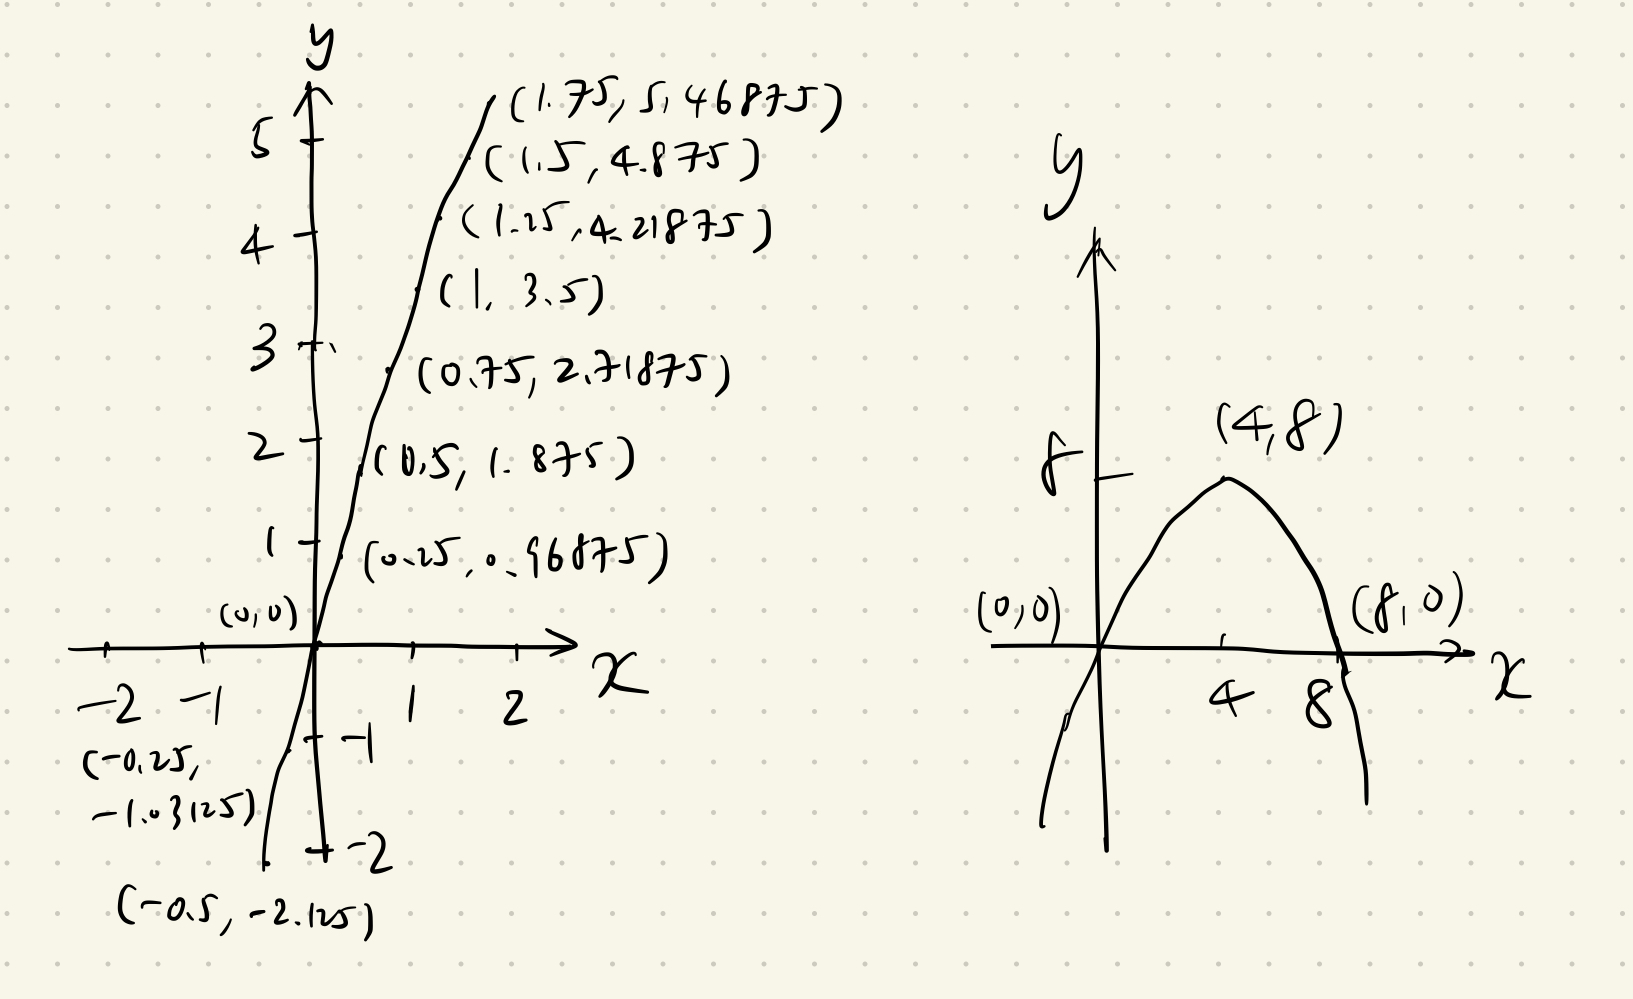
\includegraphics[width = 0.75\textwidth]{figures/chap 05/sketching_demo.png}
    \label{fig: sketching_demo}
\end{figure}

Up until now, we have already known how to tap into several features of a function $f(x)$, including:
\begin{itemize}
    \item Discontinuities and behavior at discontinuities: Find values $c$ where $f(c)$ is undefined, or where $\lim_{x\rightarrow c}f(x) \ne f(c)$. The latter usually happens when $f(x)$ is piecewise defined.  We can then try to evaluate $f(c)$, $\lim_{x \rightarrow c^+}f(x)$ and $\lim_{x \rightarrow c^-}f(x)$ to ascertain the behavior of $f(x)$ around and at $x=c$.
    \item Behavior at boundaries: We may evaluate the behavior of the function at its domain boundaries by taking its limit at that boundary. For example, if the domain of $f$ is $(\ell, u)$, then we can try to evaluate $\lim_{x \rightarrow \ell^+}f(x)$ and $\lim_{x \rightarrow u^-}f(x)$ and see if the function converge to a value, or blows up to $\pm \infty$.  Alternatively, if the domain is unbounded (eg. $\mathbb{R}$), we can try finding $\lim_{x \rightarrow \infty}f(x)$ and $\lim_{x \rightarrow -\infty}f(x)$.
    \item $y$-intercept: Plug $0$ into $x$.
    \item $x$-intercepts (roots): Let $f(x)=0$ and solve for $x$.
\end{itemize}

Apart from the features above (which you \textit{should} include in your curve sketching if possible), as we will soon see, the behavior of the function is also largely governed by its first derivative $f'$ and second derivative $f''$.  Therefore, a big part of curve sketching is to determine where $f'$ and $f''$ are zero, positive or negative.  We will first start with the first derivative $f'$.

\subsection{First Derivative and Critical Points}

Given a function $f$, its first derivative $f'$ governs if $f$ is \textit{increasing} or \textit{decreasing}.  The concept of (strictly) increasing and decreasing is straightforward: if $f(x)$ is getting larger as $x$ is getting larger, then $f(x)$ is increasing, vice versa.  The reason why we added "(strictly)" is that by convention in mathematics, "increasing" and "decreasing" permits the possibility where $f(x)$ remains the same value as $x$ is getting larger.  This can be illustrated by the following graphs:

\begin{figure}[ht]
    \centering
    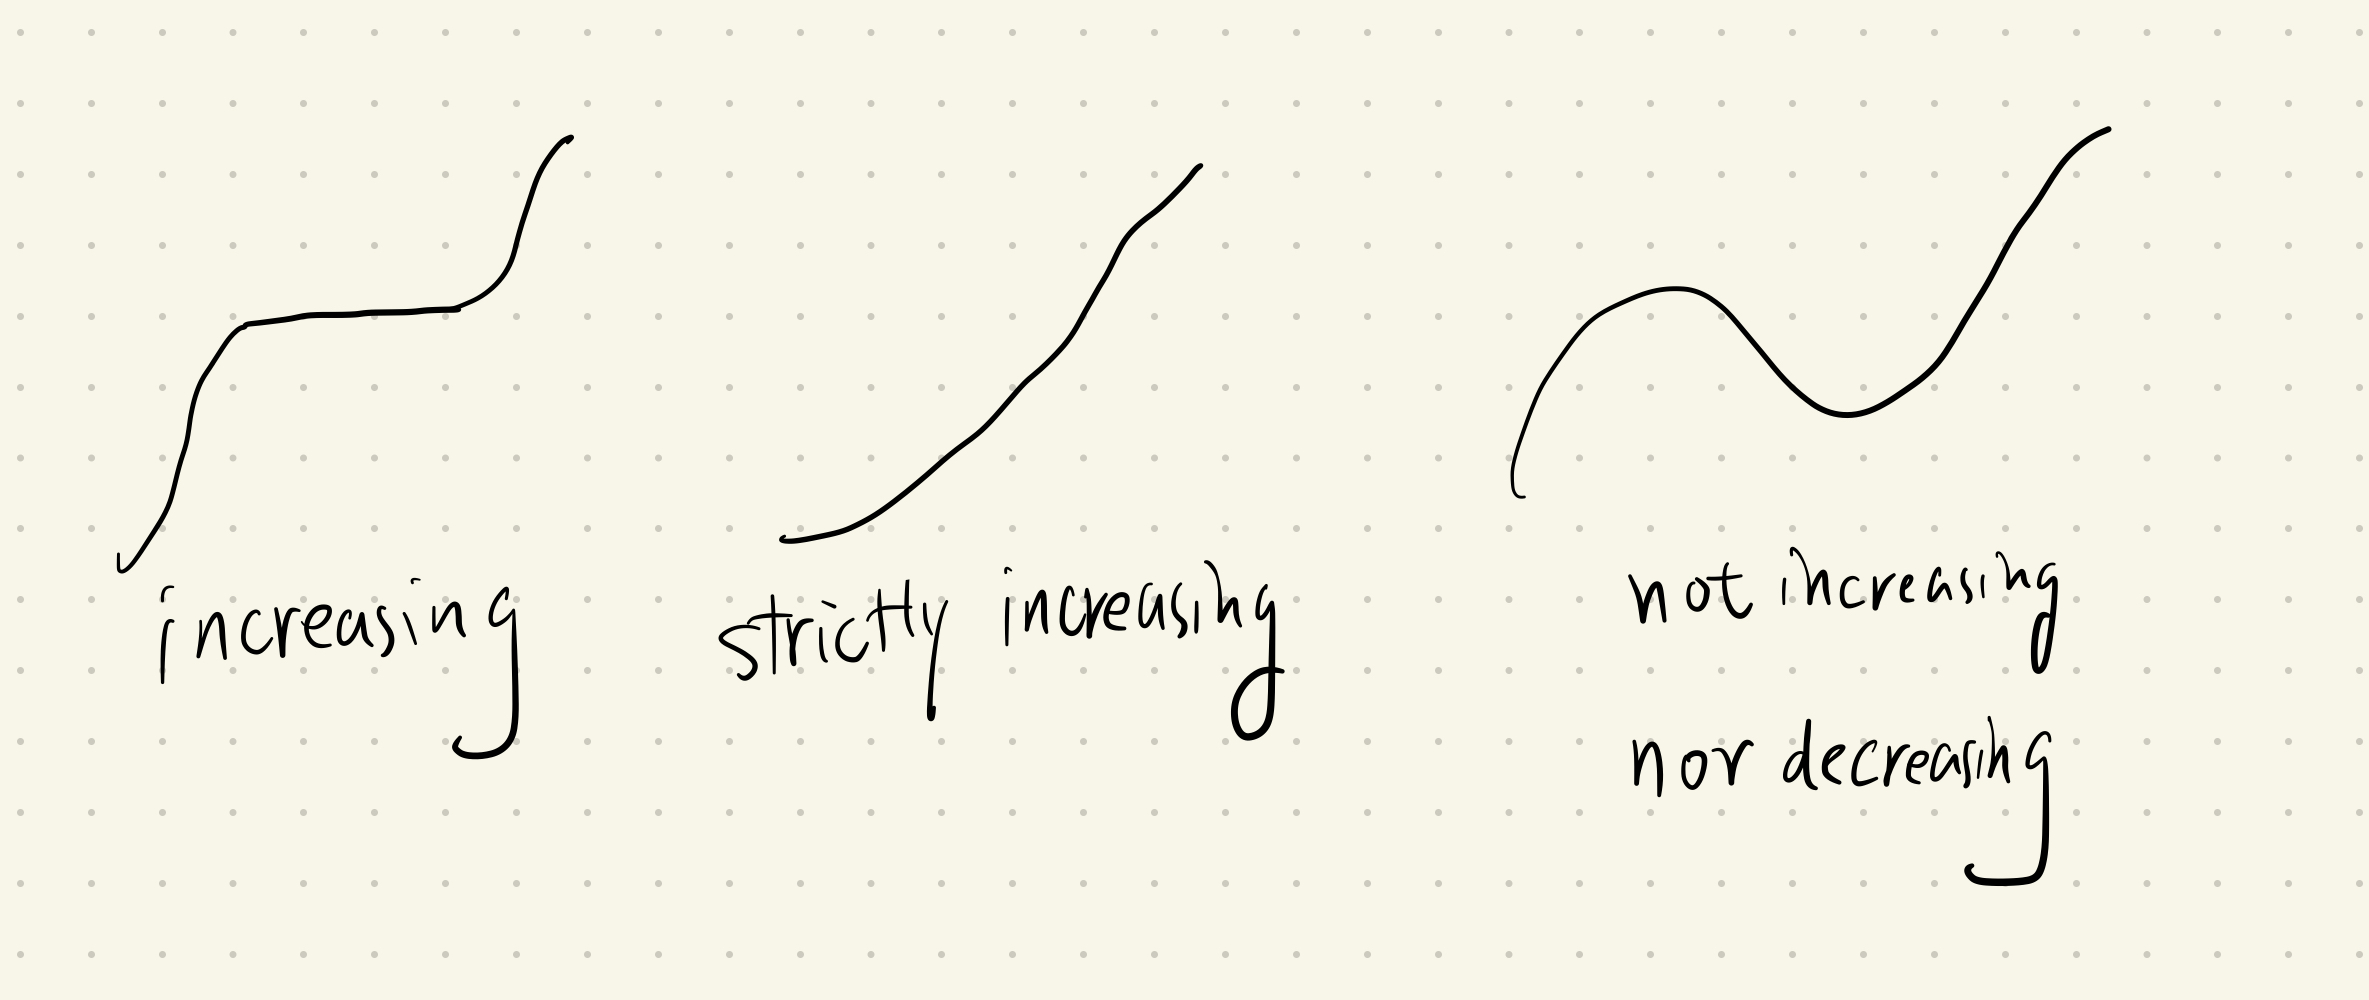
\includegraphics[width = 0.8\textwidth]{figures/chap 05/def_increasing_decreasing.png}
    \label{fig: def_increasing_decreasing}
\end{figure}

We hereby include the formal definition of increasing and decreasing functions for completeness:

\begin{defi}[Increasing and decreasing functions]{def: increasing_decreasing}
    Let $I$ be an interval and $x_1, x_2$ be any two numbers in $I$. A function $f(x)$ is:
    \begin{itemize}
        \item \textit{increasing} in $I$ if $x_1 > x_2$ implies $f(x_1) \ge f(x_2)$.
        \item \textit{strictly increasing} in $I$ if $x_1 > x_2$ implies $f(x_1) > f(x_2)$.
        \vspace{0.5cm}
        \item \textit{decreasing} in $I$ if $x_1 > x_2$ implies $f(x_1) \le f(x_2)$.
        \item \textit{strictly decreasing} in $I$ if $x_1 > x_2$ implies $f(x_1) < f(x_2)$.
    \end{itemize}
\end{defi}

To relate the derivative of a function to whether it is strictly increasing or decreasing, we can look at the following graph:
\begin{enumerate}
    \item In the left panel, the slope of the tangent lines (i.e. the derivatives) are always \textit{positive} within $(a, b)$, and we see that the function is \textit{strictly increasing} in $(a, b)$.
    \item In the right panel, the slopes of the tangent lines are always \textit{negative} within $(a, b)$, and the function is \textit{strictly decreasing} in $(a, b)$.  
\end{enumerate}
 
\pagebreak

\begin{figure}[ht]
    \centering
    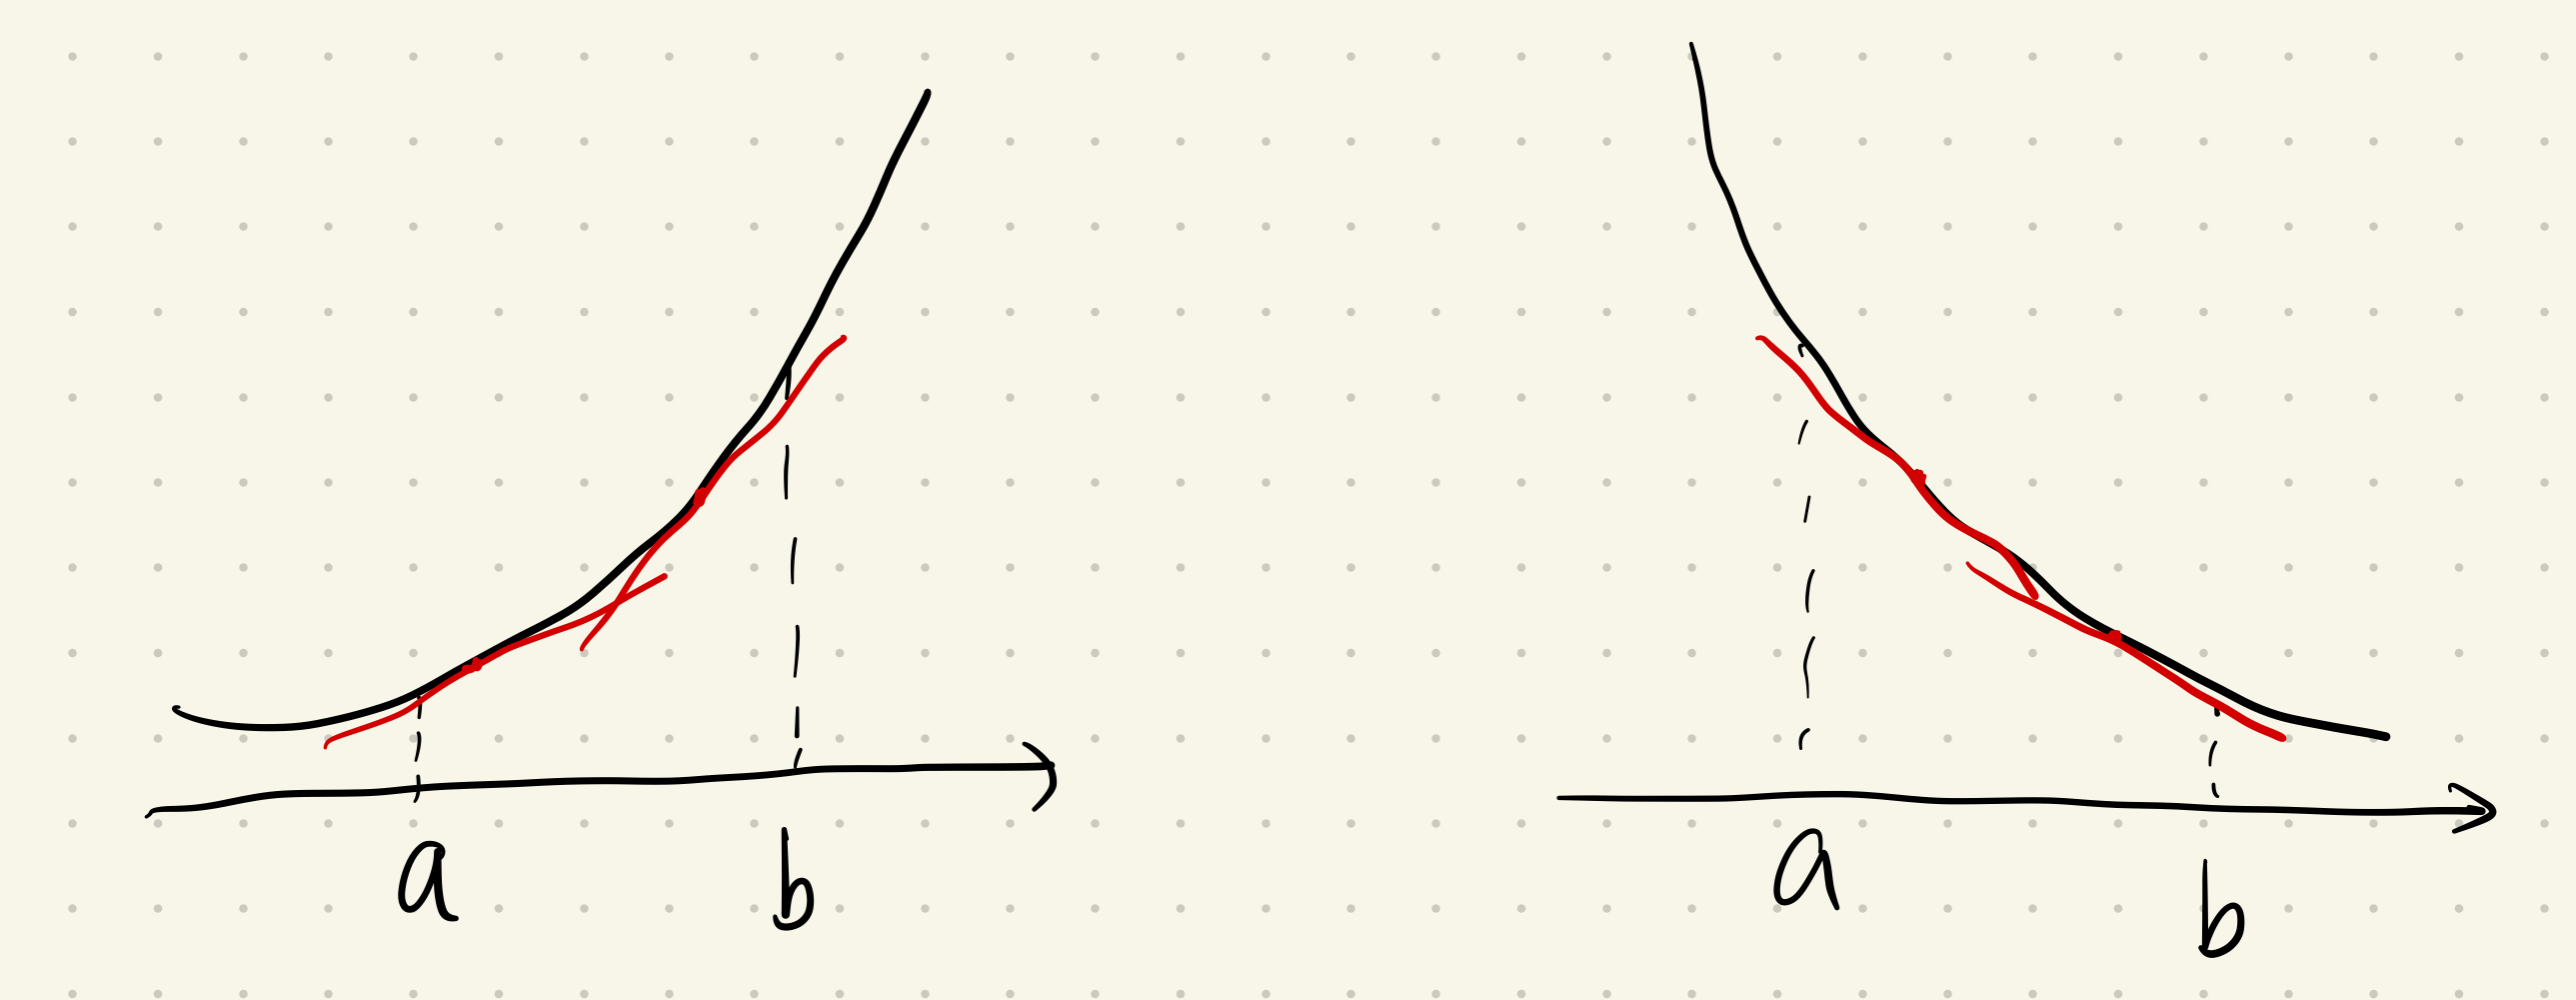
\includegraphics[width = 0.7\textwidth]{figures/chap 05/increasing_decreasing.png}
    \label{fig: increasing_decreasing}
\end{figure}

We can summarize our findings into the following theorem:

\begin{theo}[Derivative and strict monotonicity]{thm: derivative_to_monotone}
    Suppose a function $f(x)$ is differentiable in $(a, b)$, then:
    \[f'(x) > 0, \forall x \in (a, b) \Rightarrow f(x) \text{ is \textit{strictly increasing} in } (a,b)\]
    \[f'(x) < 0, \forall x \in (a, b) \Rightarrow f(x) \text{ is \textit{strictly decreasing} in } (a,b)\]
    If in addition $f(x)$ is continuous in $[a, b]$, then
    \[f'(x) > 0, \forall x \in (a, b) \Rightarrow f(x) \text{ is \textit{strictly increasing} in } [a,b]\]
    \[f'(x) < 0, \forall x \in (a, b) \Rightarrow f(x) \text{ is \textit{strictly decreasing} in } [a,b]\]
\end{theo}

We will prove this theorem rigorously in later subsections, and now we will focus on its practical use.  For a function $f(x)$, we may try to find intervals for $x$ where $f'(x)$ is positive, so we would know that $f(x)$ is strictly increasing in this region.  Likewise, we may find intervals where $f'(x)$ is negative so that $f(x)$ is strictly decreasing in that region.  This can be demonstrated with the following example:

\begin{eg}[]{eg: increasing_decreasing}
    Find intervals on which the function $f(x) = x^5 + 5x^4 - 20x^3 + 30$ is increasing or decreasing.
\end{eg}

\begin{egsol}[]{egsol: increasing_decreasing}
    We first calculate the derivative of $f(x)$, which is
    \[f'(x) = 5x^4 + 20x^3 - 60x^2 = 5x^2(x^2+4x-12) = 5x^2(x-2)(x+6)\]
    To find where $f'(x)$ is positive or negative, we can first determine where $f'(x) = 0$, i.e. find the roots for $f'(x)$.  These roots can then serve as anchor points to help us find regions where $f'(x)$ is positive or negative.
    
    Since $f'(x)$ has three distinct roots $0, 2, -6$, we can divide the number line into four regions with these three roots: $(-\infty, -6)$, $(-6, 0)$, $(0, 2)$ and $(2, \infty)$, illustrated in the graph below: 
    \begin{center}
        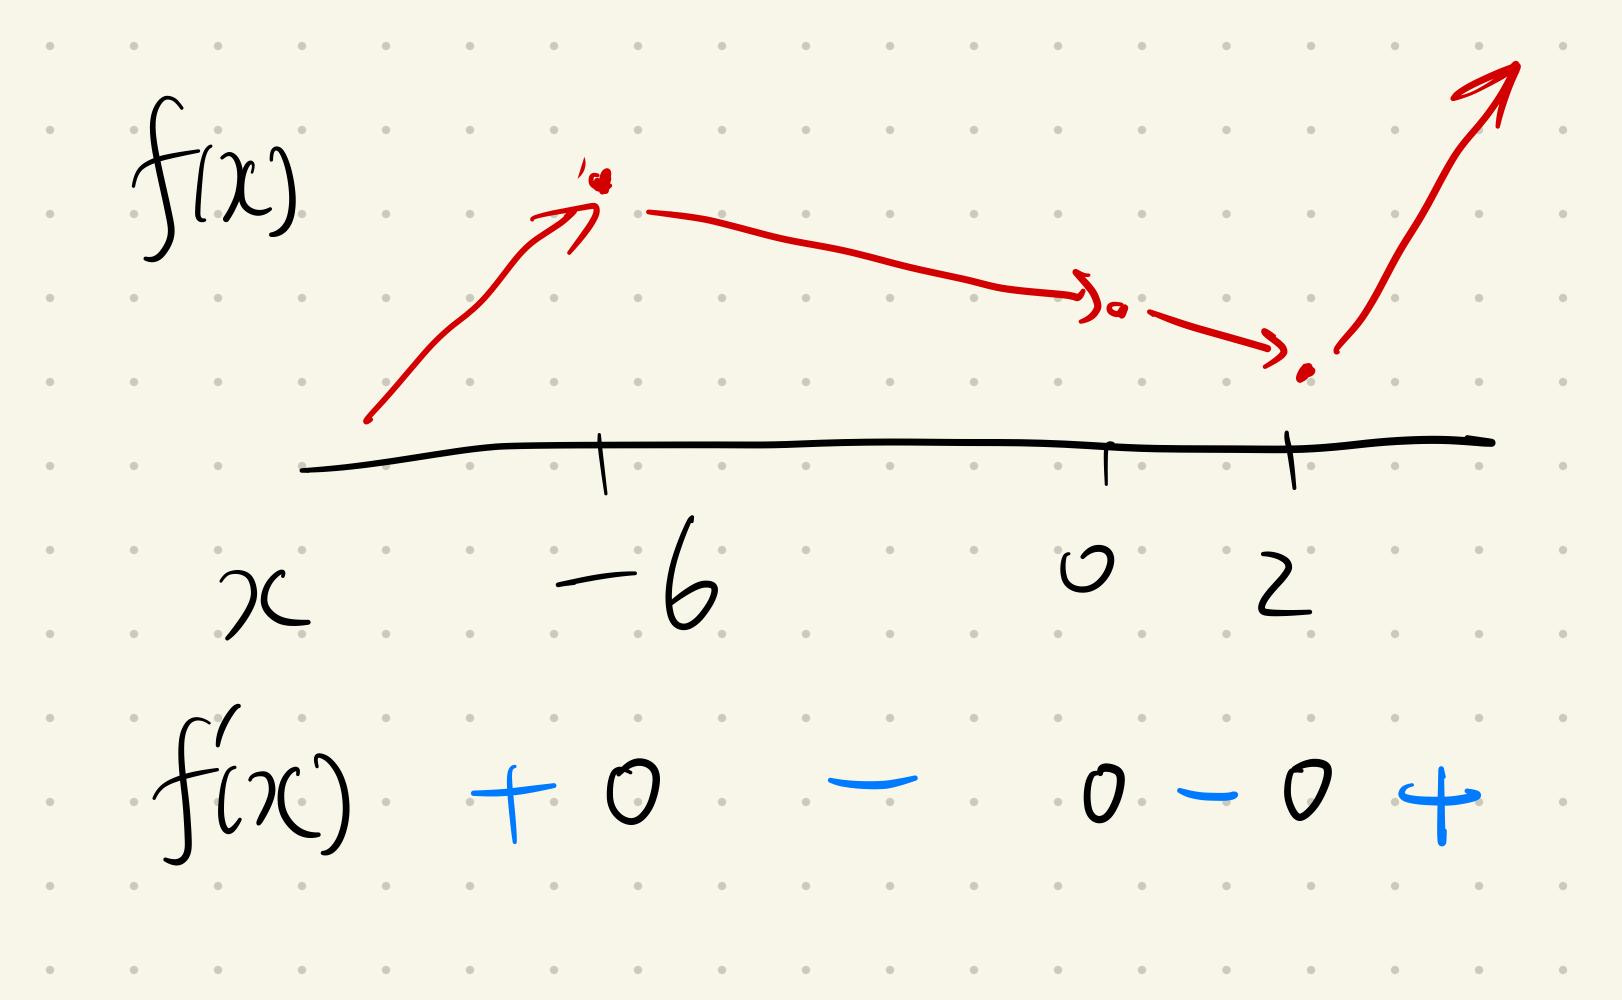
\includegraphics[width = 0.5\textwidth]{figures/chap 05/eg_increasing_decreasing.png}
        \label{fig: eg_increasing_decreasing}
    \end{center}
    We now assess the sign of $f'(x) = 5 (x+6) \cdot x \cdot x \cdot (x-2)$ in each interval by evaluating the sign of each factor, i.e. $x+6$, $x$, $x$ and $x-2$:
    \begin{itemize}
        \item $(2, \infty):$ All factors of $f'(x)$ are positive in this interval, so $f'(x)$ is positive.
        \item $(0, 2):$ We have three positive factors ($x+6$, $x$, $x$) and one negative factor ($x-2$), so $f'(x)$ is negative.
        \item $(-6, 0):$ We have one positive factor ($x+6$) and three negative factors ($x$, $x$, $x-2$), so $f'(x)$ is negative.
        \item $(-\infty, -6):$ We have all four factors negative, so $f'(x)$ is positive.
    \end{itemize}
    From Theorem~\ref{thm: derivative_to_monotone}, since $f(x)$ is a polynomial and thus differentiable and continuous in $\mathbb{R}$, it is strictly increasing in $(-\infty, -6]$ and $[2, \infty)$ and strictly decreasing in $[-6, 2]$.  We can then sketch the increasing and decreasing behavior of $f(x)$ based on our finding, also shown in the graph.
\end{egsol}

\begin{remark}
    From the graph we can see that as $x$ is increasing from the left side of the number line, $f(x)$ is increasing until $x = -6$, then it decreases until $x = 2$, then it increases again.  Therefore, $f(-6)$ and $f(2)$ are the "local maximum" and "local minimum" of the function, i.e. $f(x)$ has a peak at $x = -6$ and a valley at $x = 2$.  We will talk more about this later when we are using derivatives to obtain extrema. 
\end{remark}

\begin{remark}
    In this example, we first identified points where $f'(x) = 0$ to aid us finding intervals where $f(x)$ is increasing and decreasing.  In fact, points where $f'(x) = 0$ or $f'(x)$ is undefined carry a great deal of information on the behavior of $f(x)$, and they deserve a dedicated name defined below:
\end{remark}

\begin{defi}[Critical points and critical values]{def: crit}
    A point $x=c$ in the domain of $f(x)$ is termed as a \textit{critical point} for $f(x)$ if $f'(c) = 0$ or $f'(c)$ does not exist.  The function value $f(c)$ is then termed as a \textit{critical value} for $f(x)$ associated with the critical point $x=c$.
\end{defi}

The reason why we care about critical points is that the behavior of a function near its critical points is often interesting.  Therefore, knowing where the critical points are helps us know the function better.  For example, lets take a look at the following graph showing seven critical points of a function:

\begin{figure}[ht]
    \centering
    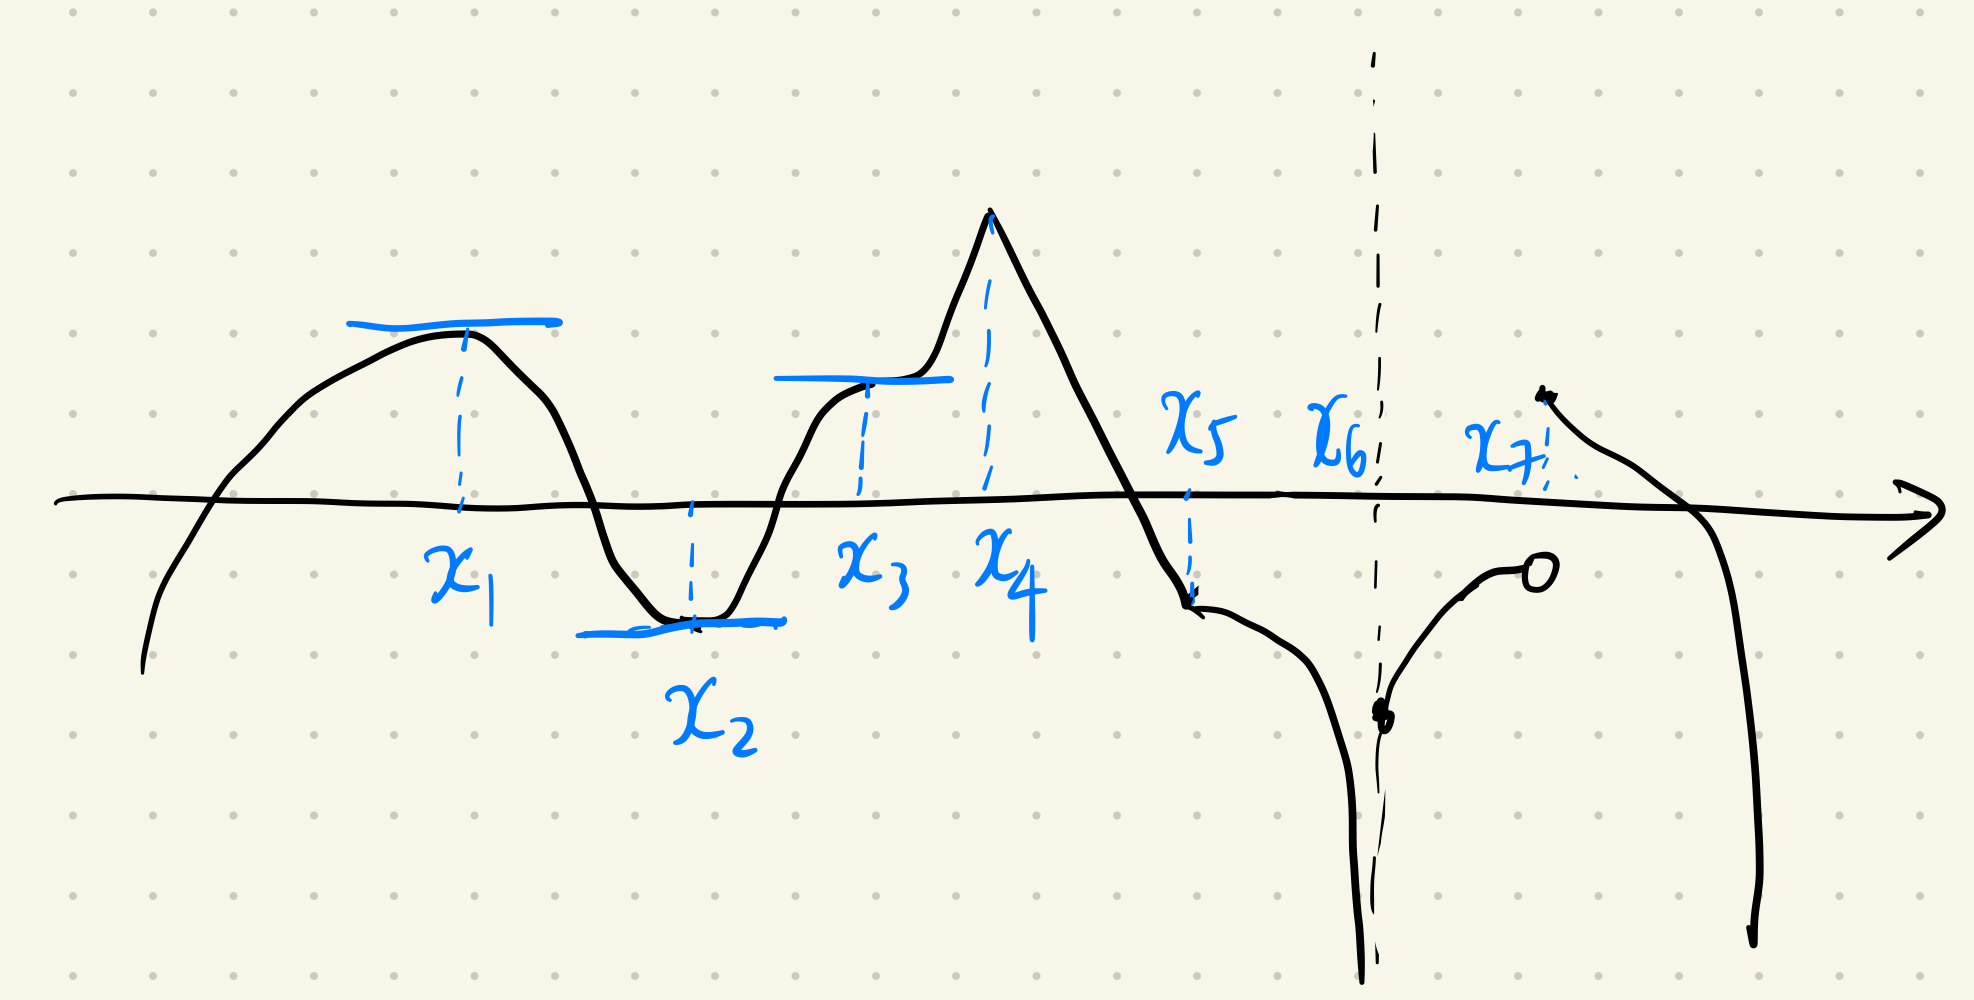
\includegraphics[width = 0.75\textwidth]{figures/chap 05/critical_points.png}
    \label{fig: critical_points}
\end{figure}

The points $x = x_1$ and $x = x_2$ are both critical points since $f'(x_1) = f'(x_2) = 0$.  These points are special since \textit{local maximum} is attained at $x = x_1$ and \textit{local minimum} is attained at $x = x_2$.

The point $x = x_3$ is also a critical point since $f'(x_3) = 0$.  This time, $x=x_3$ does not lead to local maximum or minimum, but it is an \textit{inflection point}, where the curve is turning from a bowl facing down (concave down) to a bowl facing up (concave up).  We will talk about this more when we get to second derivatives.

The points $x = x_4$ and $x = x_5$ are both critical points since $f'(x_4)$ and $f'(x_5)$ both do not exist due to a \textit{kink} in the curve.  Sometimes a local maximum and minimum will also occur at these points.  In this case, local maximum is attain at $x = x_4$.

The points $x = x_6$ and $x = x_7$ are also critical points since $f'(x_6)$ and $f'(x_7)$ both do not exist due to \textit{discontinuity}.  Finding these discontinuities will alert us that the function either has a jump or goes to $\pm\infty$, leading to better curve sketching.  Local maximum or minimum can still occur at these discontinuities, such as $x = x_7$.

With the additional information of critical points and first derivatives, we can form a procedure to sketch a function $f$ (without using second derivatives for now):

\begin{enumerate}
    \item \textit{Domain and behavior at boundaries}: Assess the behavior of $f$ at the boundary of its domain.
    \item \textit{Find discontinuities}: Find all discontinuities in $f$.
    \item \textit{Behavior at discontinuities}: Assess the behavior of $f$ at the discontinuities ($f(c)$ and the left / right limits of $f(c)$ at $x=c$).
    \item \textit{Find and plot critical points}: Find the critical points / values of $f$ (this may include some discontinuities we've found in the first step) and plot them.
    \item \textit{Behavior between critical points / discontinuities}: Assess if the function is increasing or decreasing between the critical points and discontinuities using the sign of $f'$.
    \item \textit{Miscellaneous}: (Optional) Plot "easy points" of $f$, eg. the $x$- and $y$- intercepts.
\end{enumerate}

Connecting all features in the procedure would lead to the final sketch. We now illustrate this procedure with a couple of examples.

\begin{eg}[]{eg: first_derivative}
    Find the critical points for $f(x) = \frac{2x-1}{x+1}$ and sketch $f(x)$ using the information of its first derivative.
\end{eg}

\begin{egsol}[]{egsol: first_derivative}
    To find the critical points for $f(x)$, we first find its first derivative:
    \[f'(x) = \frac{2 \cdot (x+1)-(2x-1) \cdot 1}{(x+1)^2} = \frac{3}{(x+1)^2}\]
    Therefore, $f'(x)$ is always positive except for $x = -1$ where it's undefined.  However, $x = -1$ is not in the domain of $f(x)$, so there are no critical points for $f(x)$.
    
    To sketch $f(x)$, we follow the steps of the procedure mentioned above:
    
    \begin{enumerate}
        \item \textit{Domain and behavior at boundaries}: The domain of $f(x)$ is $\mathbb{R} \backslash \{-1\}$, so we assess its limit at $\pm\infty$.  Since $f(x)$ is a rational function with polynomials of the same degree ($1$) at the numerator and denominator, we have
        \[\lim_{x \rightarrow \infty} f(x) = \lim_{x \rightarrow -\infty} f(x) = \frac{2}{1} = 2\]
        Therefore, $f(x)$ has a horizontal asymptote at $y = 2$ for both the left and right sides of the graph.
        \item \textit{Find discontinuities}: The only discontinuity in $f(x)$ is where its denominator equals zero, i.e. $x = -1$.
        \item \textit{Behavior at discontinuities}: $f(x)$ is undefined at $x=-1$.  The right-side limit at $x=-1$ is 
        \[\lim_{x \rightarrow (-1)^+} \frac{2x-1}{x+1} = \frac{-3}{0^+} = -\infty\]  
        While the left-side limit is
        \[\lim_{x \rightarrow (-1)^-} \frac{2x-1}{x+1} = \frac{-3}{0^-} = \infty\]
        Therefore, $f(x)$ has a vertical asymptote at $x = -1$, with its value shooting down to $-\infty$ on the right and up to $\infty$ on the left.
        \item \textit{Find and plot critical points}: We have shown that there are no critical points for $f(x)$
        \item \textit{Behavior between critical points / discontinuities}: We now determine the sign of $f'(x) = \frac{3}{(x+1)^2}$ in $(-\infty, 1)$ and $(1, \infty)$, which should both be positive.  Therefore, $f(x)$ is strictly increasing in both $(-\infty, 1)$ and $(1, \infty)$.
        \item \textit{Miscellaneous}: It is easy to find the $x$- and $y$-intercepts of $y=f(x)$, which are $\big(\frac{1}{2}, 0\big)$ and $(0, -1)$.  We can plot them on the graph.
    \end{enumerate}
    
    Combining the information above would lead us to the graph below:
    \begin{center}
        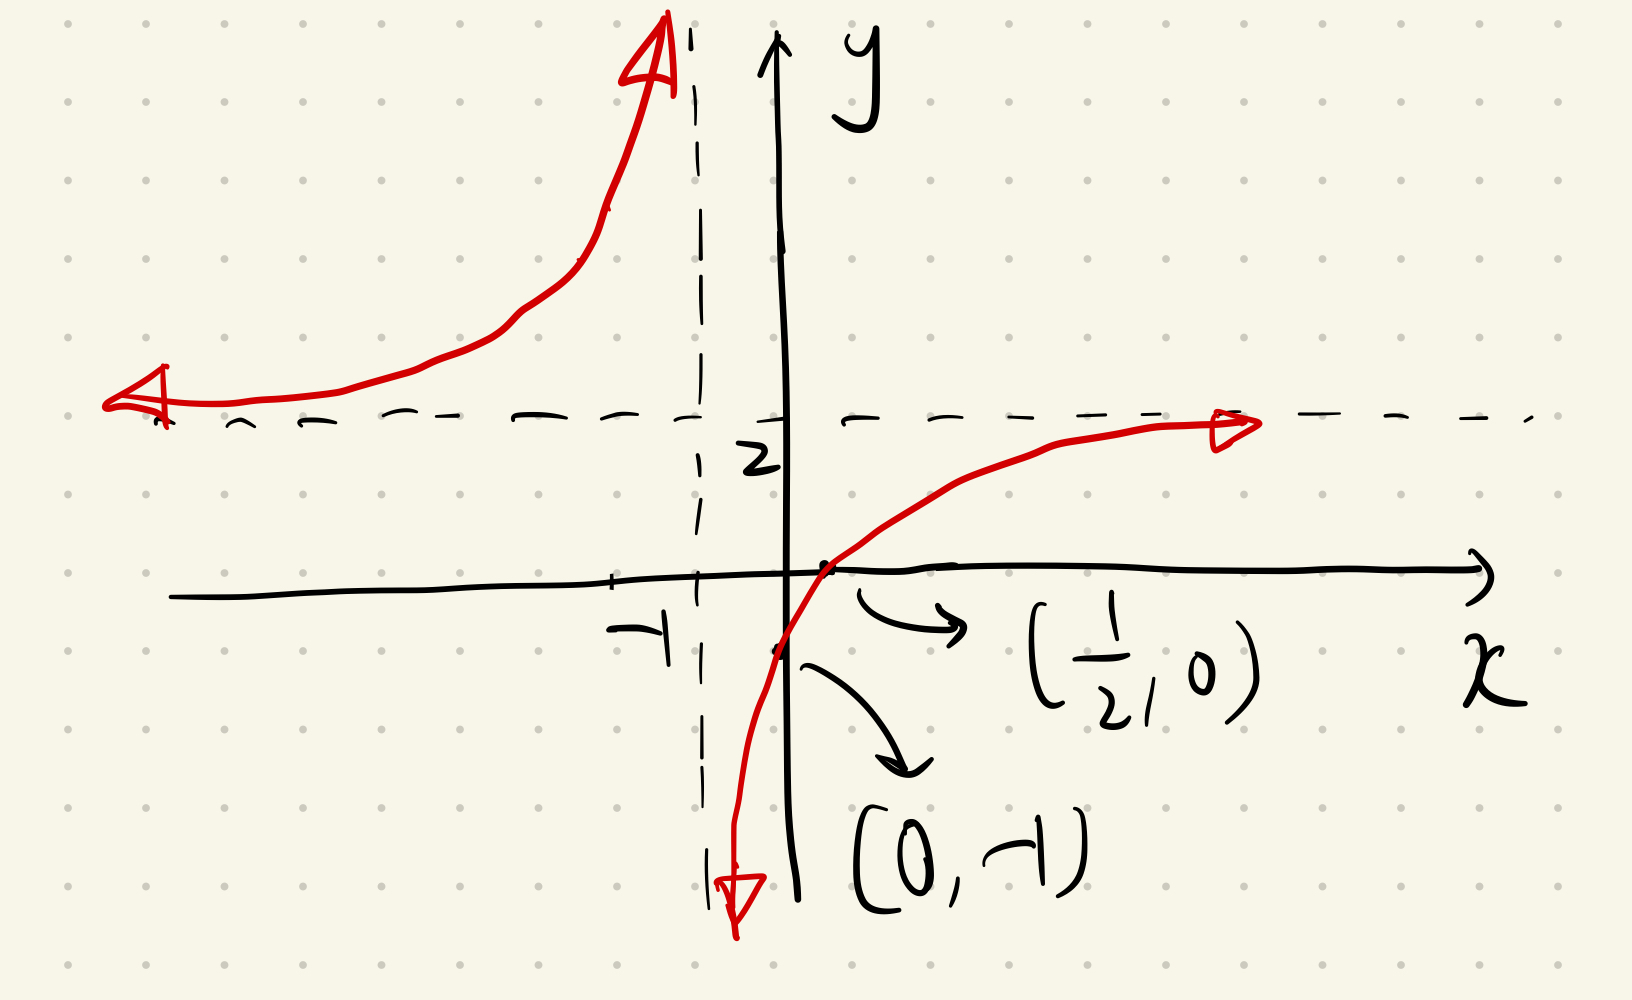
\includegraphics[width = 0.6\textwidth]{figures/chap 05/eg_first_derivative.png}
        \label{fig: eg_first_derivative}
    \end{center}
\end{egsol}

\begin{eg}[]{eg: first_derivative_2}
    Sketch $f(x)=\sqrt{x^3-3x^2+3x}$ using the information of its first derivative.
\end{eg}

\begin{egsol}[]{egsol: first_derivative_2}
    To sketch $f(x)$, we follow the steps of the procedure mentioned above:
    
    \begin{enumerate}
        \item \textit{Domain and behavior at boundaries}: Since there is a square root in the function, $f(x)$ is only defined when the expression in the square root is non-negative. That is,
        \[x^3-3x^2+3x \ge 0\]
        \[x(x^2-3x+3) \ge 0\]
        \[x\Big[\Big(x-\frac{3}{2}\Big)^2+\frac{3}{4}\Big] \ge 0\]
        Since the expression in the middle bracket is always greater than $0$, we conclude that the inequality holds if $x \ge 0$.  That is, the domain of $f(x)$ is $[0, \infty)$.
        
        As of the behavior of $f(x)$ at the boundaries, at the left boundary where $x=0$:
        \[f(0) = 0; \qquad \lim_{x\rightarrow 0^+} f(x) = 0\]
        At the right boundary, i.e. $x \rightarrow \infty$:
        \[\lim_{x\rightarrow \infty} f(x) = \lim_{x\rightarrow \infty} \sqrt{x^3} = \infty\]
        Therefore, $f(x)$ is cut off on the left at $(0,0)$ and goes to $\infty$ on the right as $x \rightarrow \infty$.
        \item \textit{Find discontinuities}: There are no discontinuities in $f(x)$.
        \item \textit{Behavior at discontinuities}: There are no discontinuities in $f(x)$.
        \item \textit{Find and plot critical points}: To find the critical points, we first calculate the derivative:
        \[f'(x) = \frac{(x^3-3x^2+3x)'}{2\sqrt{x^3-3x^2+3x}} = \frac{3x^2-6x+3}{2\sqrt{x^3-3x^2+3x}} = \frac{3}{2\sqrt{x^3-3x^2+3x}}(x-1)^2\]
        Therefore, there is only one critical point, which is $x = 1$ where $f'(1) = 0$.  We can then plot the point $(1,f(1)) = (1,1)$ on the plane.
        \item \textit{Behavior between critical points / discontinuities}: We now determine the sign of $f'(x) = \frac{3}{2\sqrt{x^3-3x^2+3x}}(x-1)^2$ in $[0, 1)$ and $(1, \infty)$, which are all positive.  Therefore, $f(x)$ is strictly increasing in both $[0, 1)$ and $(1, \infty)$.  Note that since $f'(1) = 0$, we must sketch in a way that the tangent line at $x=1$ is horizontal.
        \item \textit{Miscellaneous}: We may try to plot other points, but here we do not see any obvious choices.
    \end{enumerate}
    
    Combining the information above would lead us to the graph below:
    \begin{center}
        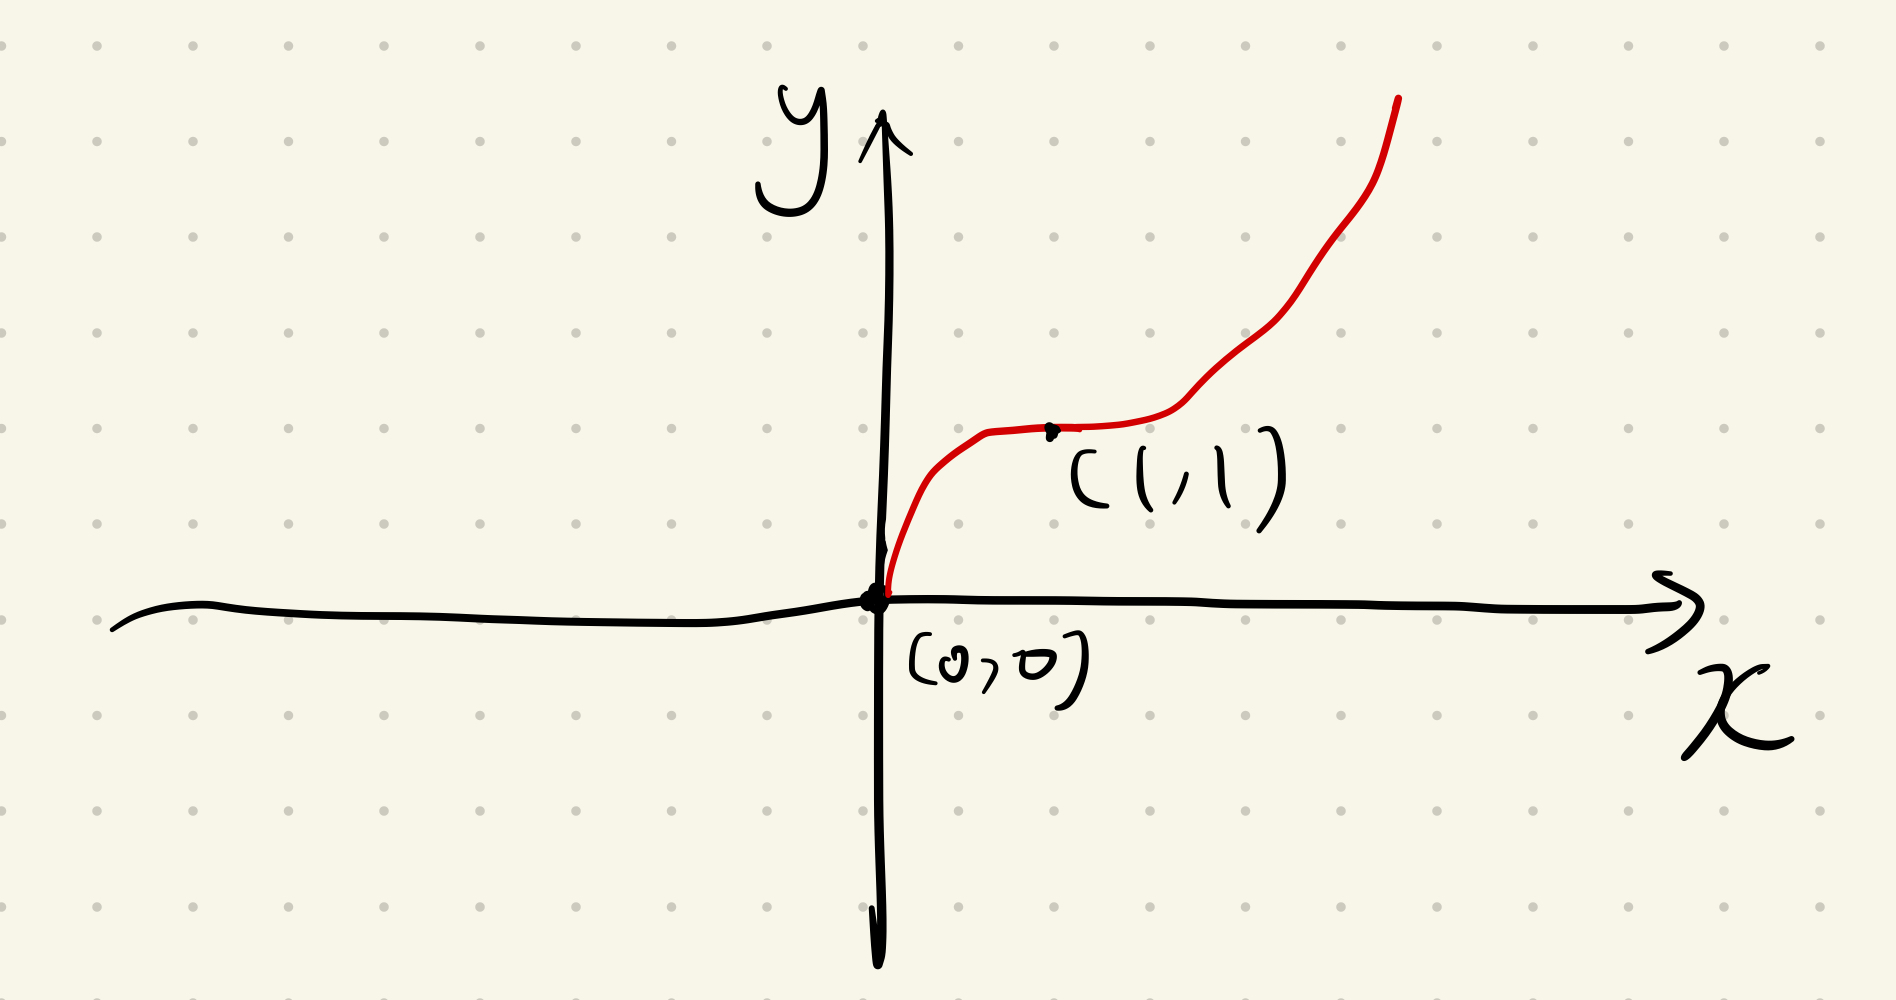
\includegraphics[width = 0.6\textwidth]{figures/chap 05/eg_first_derivative_2.png}
        \label{fig: eg_first_derivative_2}
    \end{center}
\end{egsol}

\begin{ex}[]{ex: first_derivative}
    Sketch $f(x)=\frac{\ln x}{x}$ using the information of its first derivative.
\end{ex}

\begin{exsol}[]{exsol: first_derivative}
    To sketch $f(x)$, we follow the steps of the procedure mentioned above:
    
    \begin{enumerate}
        \item \textit{Domain and behavior at boundaries}: $f(x)$ is only defined if (1) $\ln x$ is defined, i.e. $x > 0$ (2) the denominator $x$ is non-zero, i.e. $x \ne 0$.  Combining these two conditions and we yield the domain of $f(x)$ which is $(0, \infty)$.
        
        As of the behavior of $f(x)$ at the boundaries, at the left boundary where $x=0$, $f(0)$ is undefined, and we have the limit:
        \[\lim_{x\rightarrow 0^+} \frac{\ln x}{x} = \frac{-\infty}{0+} = -\infty\]
        At the right boundary, i.e. $x \rightarrow \infty$, plug-in method yields $\frac{\infty}{\infty}$, so we use the L'Hôpital's rule:
        \[\lim_{x\rightarrow \infty} \frac{\ln x}{x} = \lim_{x\rightarrow \infty} \frac{(\ln x)'}{x'} = \lim_{x\rightarrow \infty} \frac{1/x}{1} = 0\]
        Therefore, $f(x)$ goes to $-\infty$ as $x$ goes to $0$, and as $x \rightarrow \infty$, we have a horizontal asymptote $y = 0$.
        \item \textit{Find discontinuities}: There are no discontinuities in $f(x)$.
        \item \textit{Behavior at discontinuities}: There are no discontinuities in $f(x)$.
        \item \textit{Find and plot critical points}: To find the critical points, we first calculate the derivative:
        \[f'(x) = \frac{(\ln x)'x - (\ln x)x'}{x^2} = \frac{\frac{1}{x}x - \ln x}{x^2} = \frac{1-\ln x}{x^2}\]
        Therefore, there is only one critical point, which is $x = e$ where $f'(e) = 0$.  We can then plot the point $(e,f(e)) = (e,1/e)$ on the plane.
        \item \textit{Behavior between critical points / discontinuities}: We now determine the sign of $f'(x) = \frac{1-\ln x}{x^2}$, which is positive in $(0, e)$ and negative in $(e, \infty)$.  Therefore, $f(x)$ is strictly increasing in $(0, e)$ but strictly decreasing in $(e, \infty)$.
        \item \textit{Miscellaneous}: Since $f(x)$ has an obvious root $x=1$, we can plot $(1,0)$ in the graph.
    \end{enumerate}

    Combining the information above would lead us to the graph below:
    
    \begin{center}
        \includegraphicsex{width = 0.6\textwidth, draft}{width = 0.6\textwidth}{figures/chap 05/ex_first_derivative.png}
        \label{fig: ex_first_derivative}
    \end{center}
\end{exsol}

\subsection{Second Derivative and Concavity}
The second derivative is the derivative of the first derivative, so we can apply Theorem~\ref{thm: derivative_to_monotone} to $f'(x)$ and conclude that $f''(x) > 0$ implies $f'(x)$ is strictly increasing, and $f''(x) < 0$ implies $f'(x)$ is strictly decreasing.  But when $f'(x)$ is strictly increasing / decreasing, what is its implication on the graph of $f(x)$?  To grasp intuition, let's look at the following graph of a function:

\begin{figure}[ht]
    \centering
    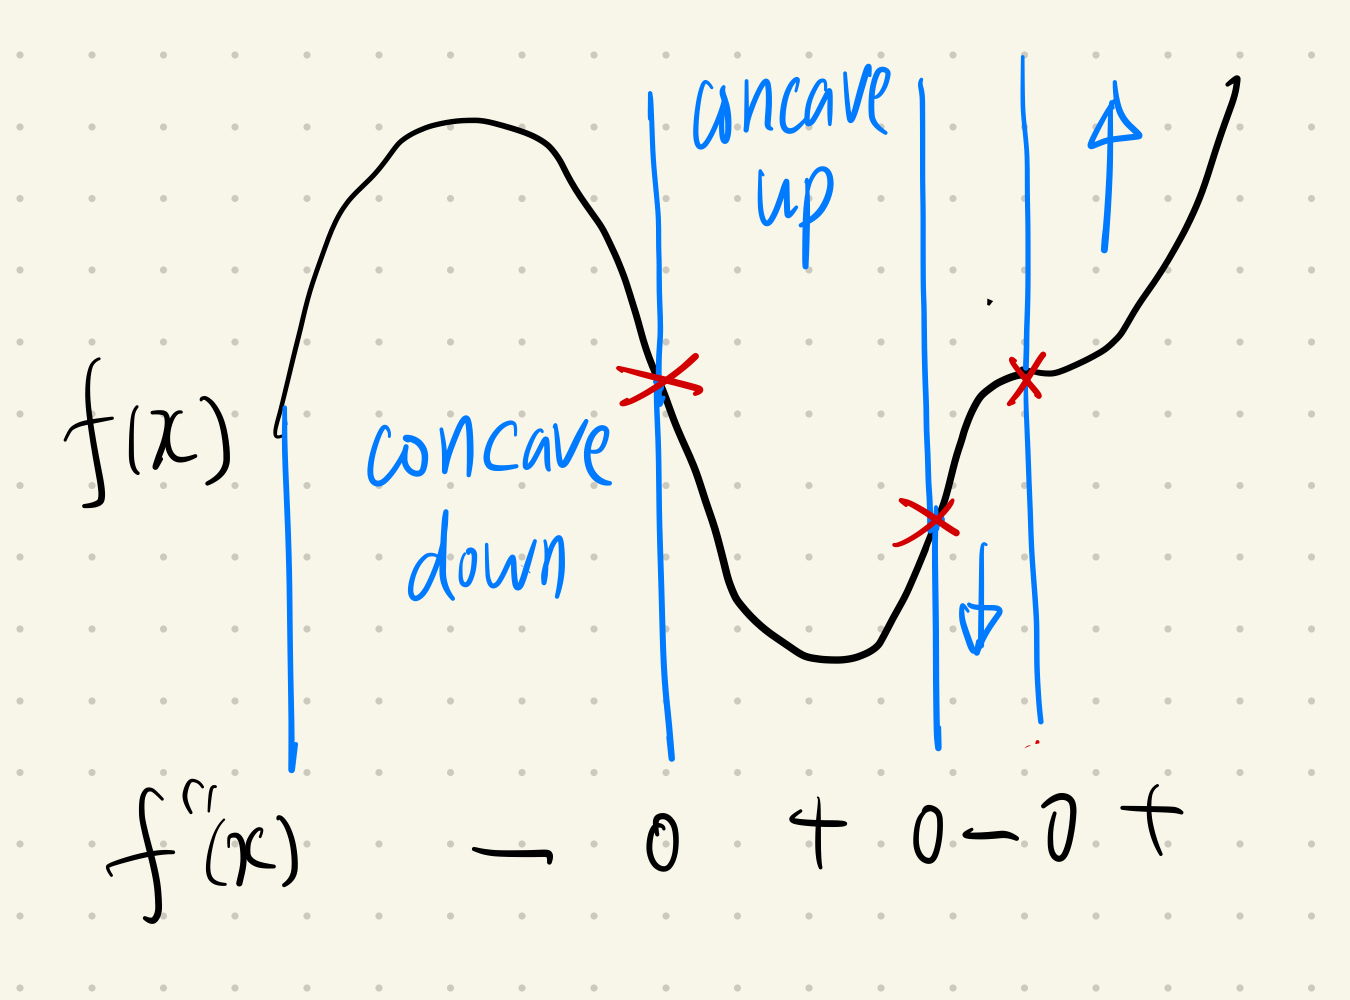
\includegraphics[width = 0.5\textwidth]{figures/chap 05/concavity.png}
    \label{fig: concavity}
\end{figure}

We first investigate the intervals marked as "\textit{concave down}" (or with a downward arrow).  Within these intervals, as $x$ gets larger, the slope of the tangent line decreases, which corresponds to $f'(x)$ \textit{decreasing}.  Note that the graph of $f(x)$ in these intervals resembles a bowl facing down, thus the term "concave down".  

In contrast, within intervals marked as "\textit{concave up}" (or with an upward arrow), the slope of the tangent line increases as $x$ gets larger, which corresponds to $f'(x)$ \textit{increasing}.  The graph of $f(x)$ in these intervals resemble a bowl facing up, thus the term "concave up".

An alternative view of curves concaving up and down is to imagine you are driving a car along the curve to the right.  If the curve is concaving down, then you are turning right along the way.  If the curve is concaving up, then you are turning left along the way.

With the concept of concavity, we can state a theorem very close to Theorem~\ref{thm: derivative_to_monotone}, but for the second derivative:

\begin{theo}[Second derivative and concavity]{thm: second_derivative_to_concavity}
    Suppose a function $f(x)$ is twice differentiable in $(a, b)$, then:
    \[f''(x) > 0, \forall x \in (a, b) \Rightarrow f(x) \text{ is \textit{concave up} in } (a,b)\]
    \[f''(x) < 0, \forall x \in (a, b) \Rightarrow f(x) \text{ is \textit{concave down} in } (a,b)\]
\end{theo}

Note that in the graph, there are points at the border of the concavity intervals (marked with x) where the function transitions from concave down to concave up.  That is, $f''(x)$ has opposite signs at the two sides of the point.  These points are called \textit{inflection points}, which we provide the definition as follows:  

\begin{defi}[]{def: inflection_point}
    A point $x=c$ is the inflection point of $f(x)$ if $f(x)$ is continuous at $x=c$ and the concavity of $f(x)$ changes at the two sides of $x=c$.
\end{defi}

Since $f''(x) > 0$ and $f''(x) < 0$ implies the curve is still concaving up or down around the point, the second derivatives at inflection points should either be $0$ or do not exist.  Therefore, to find inflection points, we can find points where $f''(x) = 0$ or do not exist, then check if $f(x)$ is continuous at these points, and also if $f''(x)$ has different signs at the left and right of these points.  This procedure is analogous to what we're doing in finding critical points.

\begin{remark}
    Concavity has a deep impact on the complexity of finding the maximum and minimum of a function using algorithms (eg. Newton's method).  If the whole function is concave up (down), then finding the minimum (maximum) of the function will be relatively easy, since the function is shaped like a big valley (peak) with one minimum (maximum), and you can find the solution easily with the help of derivatives.  However, if the function is somewhere concave up and somewhere concave down, then the curve of the function can be rugged, and you may have a hard time finding the minimum or maximum if your choice of initial value is sub-optimal.
\end{remark}

\begin{figure}[ht]
    \centering
    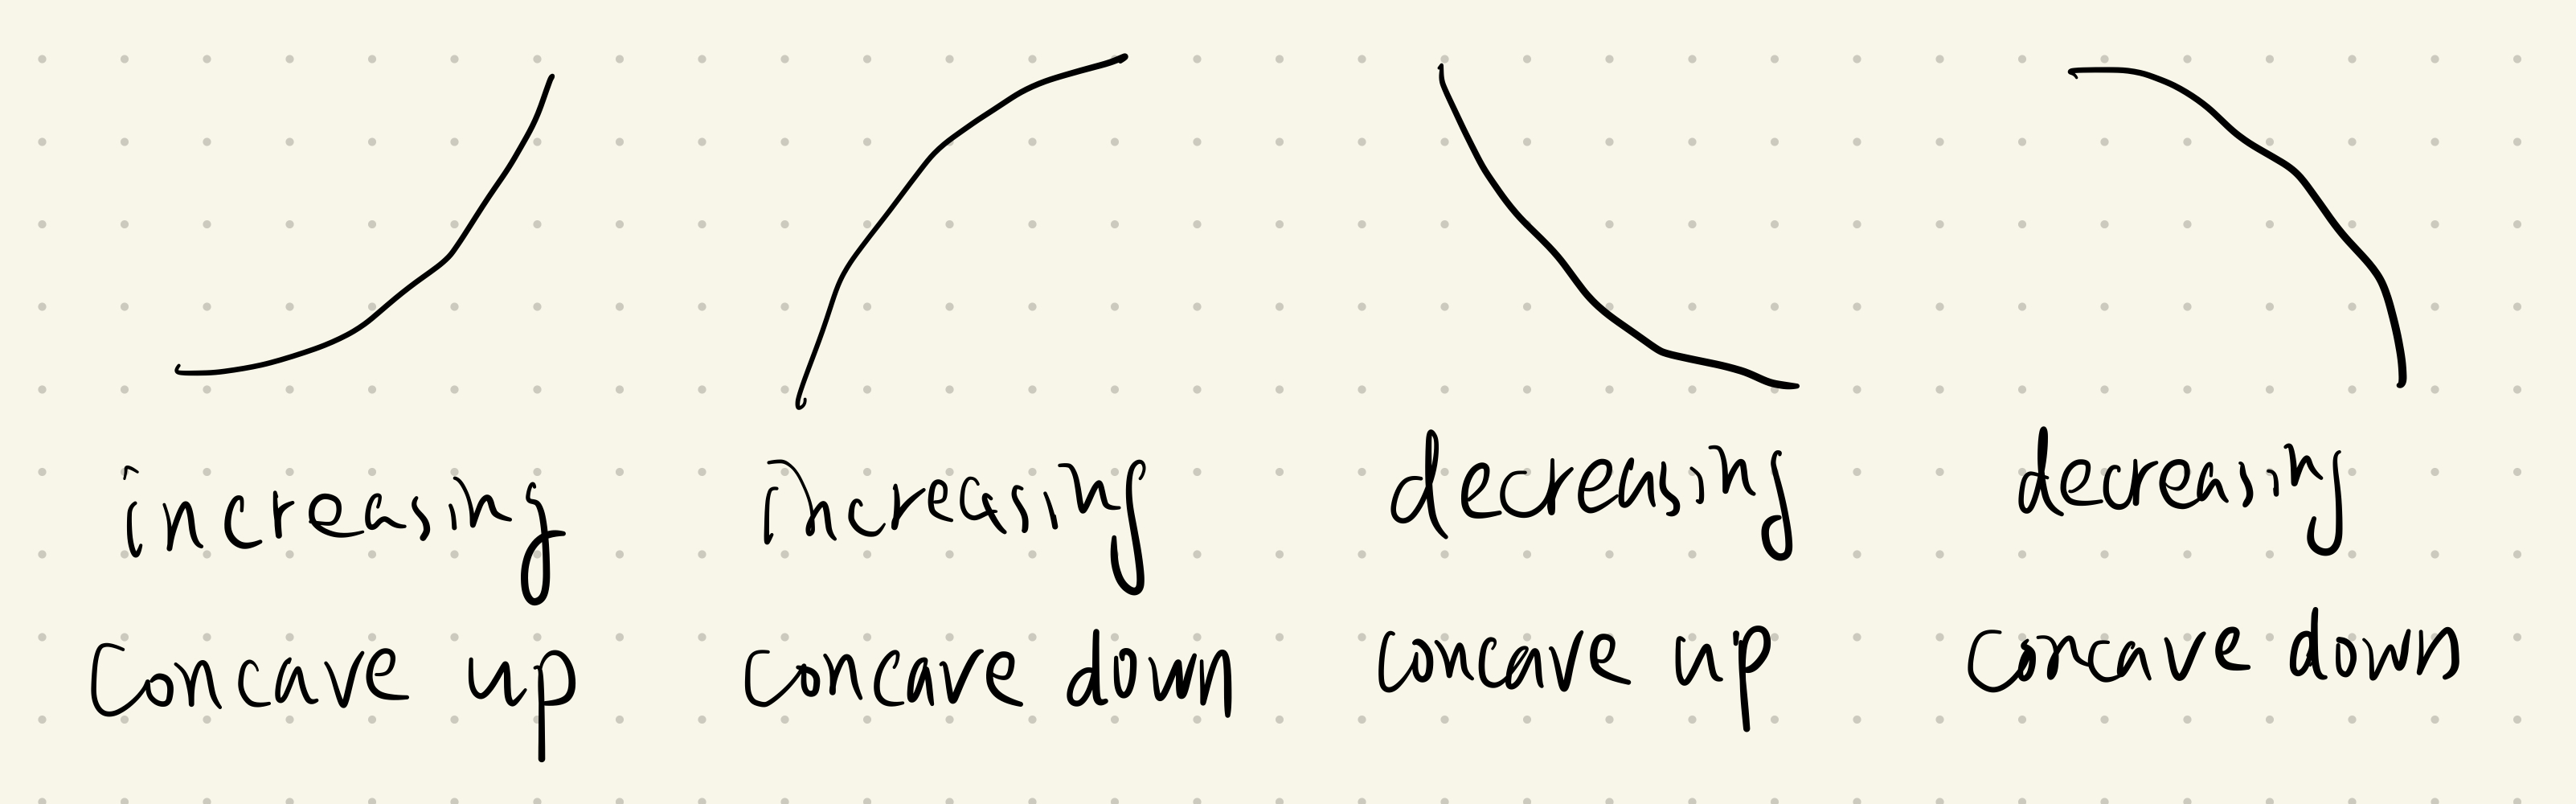
\includegraphics[width = 0.75\textwidth]{figures/chap 05/concavity_monotone.png}
    \label{fig: concavity_monotone}
\end{figure}

A word of caution is that the increasing / decreasing of a function is related to its \textit{first} derivative, and the concavity of a function is related to its \textit{second} derivative, so be careful not to mix up these two qualities of a function.  In fact, as the graph above shows, every combination between increasing / decreasing and concaving up / down is possible.

To incorporate the information of second derivatives into curve sketching, we can try finding all inflection points and incorporate the concavity of the function into our sketch after we're done with first derivatives.  We will demonstrate this with one example before ending this section. 

\begin{eg}[]{eg: second_derivative}
    Sketch $f(x) = xe^{4x}$ using the information of its first and second derivatives.
\end{eg}

\begin{egsol}[]{egsol: second}
    To sketch $f(x)$, we follow the steps of the procedure mentioned in the last subsection, but adding the inference from second derivatives:
    
    \begin{enumerate}
        \item \textit{Domain and behavior at boundaries}: The domain of $f(x)$ is $\mathbb{R}$, so we need to assess its behavior as $x \rightarrow -\infty$ and $x \rightarrow \infty$ (L'Hôpital's rule is used for $x \rightarrow -\infty$ since plug-in method leads to $-\infty \cdot 0$). 
        \[\lim_{x \rightarrow -\infty} xe^{4x} = \lim_{x \rightarrow -\infty} \frac{x}{e^{-4x}} = \lim_{x \rightarrow -\infty} \frac{x'}{(e^{-4x})'} = \lim_{x \rightarrow -\infty} \frac{1}{-4e^{-4x}} = 0\]
        \[\lim_{x \rightarrow \infty} xe^{4x} = \infty\]
        Therefore, on the left, $f(x)$ has a horizontal asymptote $y=0$; on the right, $f(x)$ goes to $\infty$ as $x$ goes to $\infty$.
        \item \textit{Find discontinuities}: There are no discontinuities in $f(x)$.
        \item \textit{Behavior at discontinuities}: There are no discontinuities in $f(x)$.
        \item \textit{Find and plot critical points}: To find the critical points, we first calculate the derivative:
        \[f'(x) = (x)'e^{4x} + x(e^{4x})' = e^{4x} + 4xe^{4x} = (4x+1)e^{4x}\]
        Therefore, there is only one critical point, which is $x = -\frac{1}{4}$ where $f'\big(-\frac{1}{4}\big) = 0$.  We can then plot the point $\big(-\frac{1}{4},f\big(-\frac{1}{4}\big)\big) = \big(-\frac{1}{4},-\frac{1}{4e})$ on the plane.
        \item \textit{Behavior between critical points / discontinuities}: We now determine the sign of $f'(x) = (4x+1)e^{4x}$ in $\big(-\infty, -\frac{1}{4}\big)$ and $\big(-\frac{1}{4}, \infty\big)$.  Since $e^{4x}$ is always non-negative, the sign of $f'(x)$ depends on the sign of $(4x+1)$.  Therefore, $f(x)$ is strictly decreasing in $\big(-\infty, -\frac{1}{4}\big)$ and strictly increasing in $\big(-\frac{1}{4}, \infty\big)$.
        \item \textit{Plot inflection points and assess concavity}: To find the inflection points, we calculate the second derivative:
        \[f''(x) = (4x+1)'e^{4x} + (4x+1)(e^{4x})' = 4e^{4x} + 4(4x+1)e^{4x} = (16x+8)e^{4x}\]
        Therefore, the only candidate for the inflection point is $x = -\frac{1}{2}$ where $f''\big(-\frac{1}{2}\big) = 0$.  
        
        To verify $x = -\frac{1}{2}$ is indeed an inflection point, we have to show that $f''(x)$ has opposite signs at different sides of $x = -\frac{1}{2}$:
        \[x < -\frac{1}{2} \Rightarrow 16x+8 < 0 \Rightarrow f''(x) = (16x+8)e^{4x} < 0\]
        \[x > -\frac{1}{2} \Rightarrow 16x+8 > 0 \Rightarrow f''(x) = (16x+8)e^{4x} > 0\]
        Therefore, $x = -\frac{1}{2}$ is an inflection point and we plot $\big(-\frac{1}{2},f\big(-\frac{1}{2}\big)\big) = \big(-\frac{1}{2},-\frac{1}{2e^2})$ on the graph, and keep in mind that $f(x)$ is concave down when $x < -\frac{1}{2}$ and concave up when $x > -\frac{1}{2}$.
        \item \textit{Miscellaneous}: An easy point to plot is $(0, f(0)) = (0, 0)$, so we add it to the graph
    \end{enumerate}
    
    Combining the information above would lead us to the graph below:
    \begin{center}
        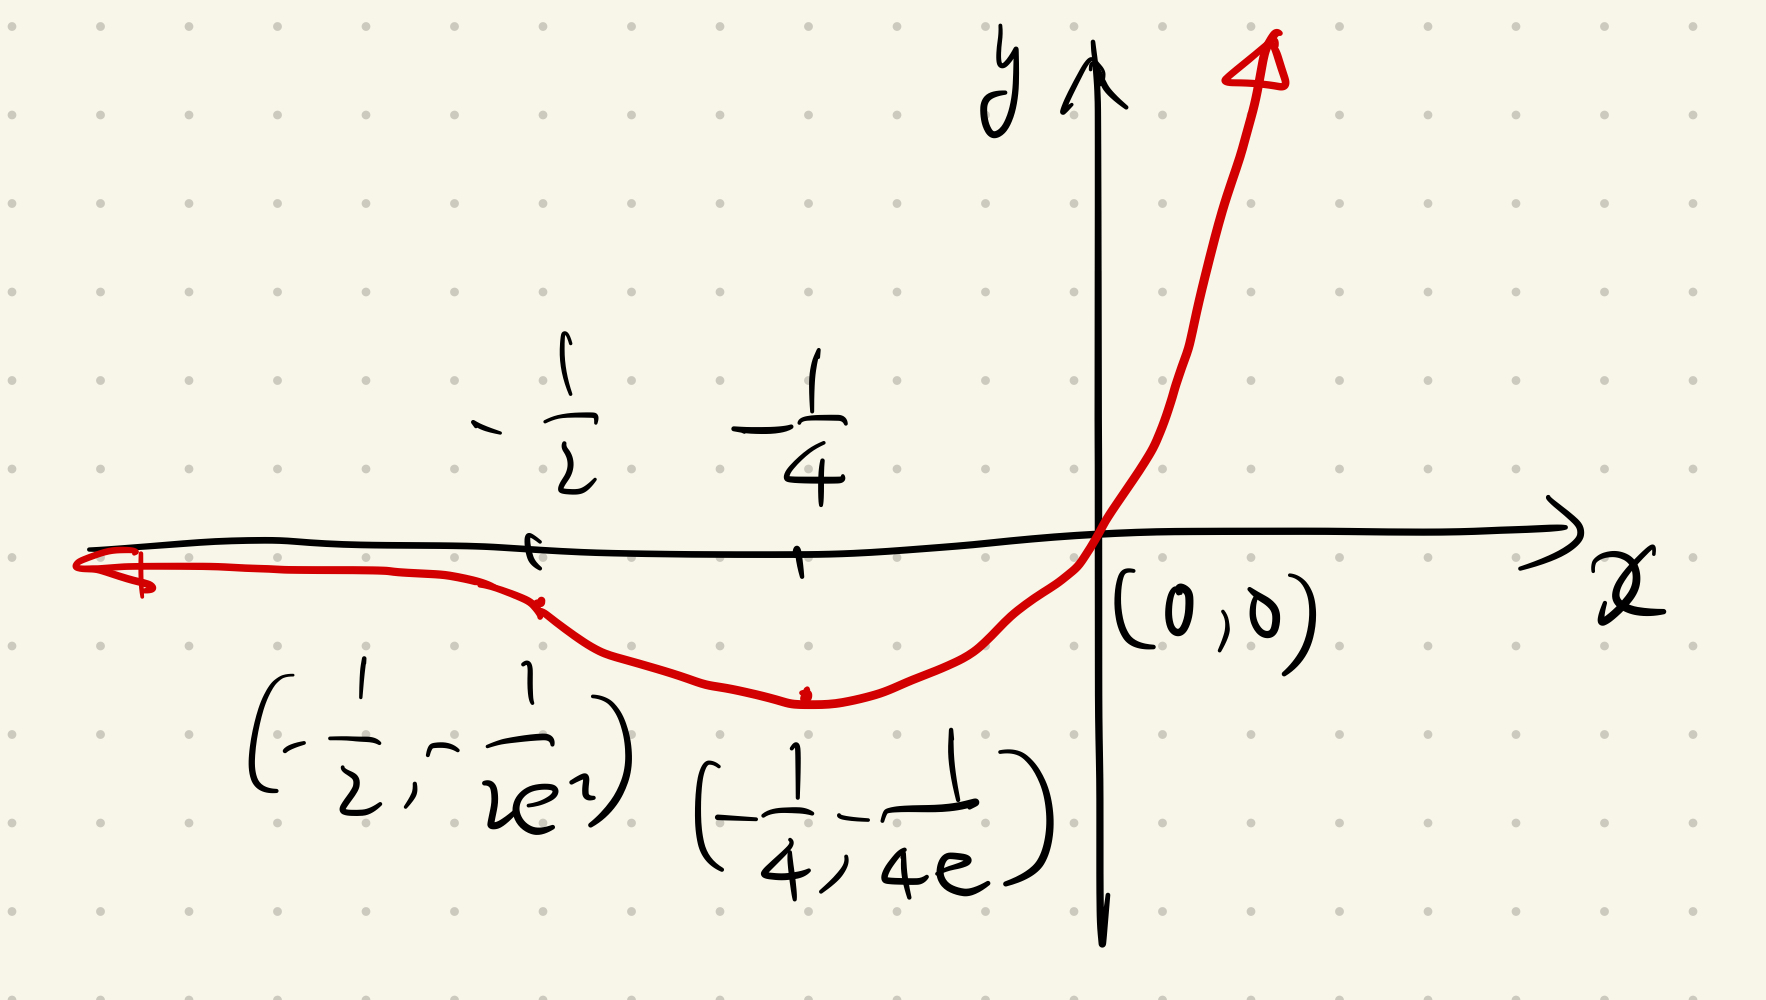
\includegraphics[width = 0.6\textwidth]{figures/chap 05/eg_second_derivative.png}
        \label{fig: eg_second_derivative}
    \end{center}
\end{egsol}

\pagebreak
\section{Finding the Extrema of a Function}

Another important use of derivatives is to determine the maximum or minimum of a function within an interval of input.  Since maxima and minima are where the function values are at their extremes, we also term them as \textit{extrema}.  Before we look into how to find the extrema of a function, we first look at the two types of extrema, \textbf{global (absolute) extrema} and \textbf{local (relative) extrema}.  

\subsection{Definition of Extrema}

Global extrema are easy to understand: it is the maximal (minimal) value the function can output.  In mathematical terms, if a function $f$ is attaining value $f(c)$ at $x=c$, and any other possible function values are less than or equal to $f(c)$, then we say $f(x)$ has a global maximum at $x=c$.  Similar arguments can be made for global minimum.  

Local extrema are a little bit more involved: If a function $f$ is attaining value $f(c)$ at $x=c$ so that all inputs \textit{around} $x=c$ are giving values less than or equal to $f(c)$, then we say $f(x)$ has a local maximum at $x=c$.  Similar arguments can be made for global maximum.  Note that here we are using the term \textit{around} in a sense that we must be able to compare $f(c)$ with function values with input less than $c$ and greater than $c$.  Therefore, the local extrema can never attained at $x=c$ if $x=c$ is at the boundary of the interval of input, since we cannot compare $f(c)$ with function values evaluated at both sides of $c$.

\begin{figure}[ht]
    \centering
    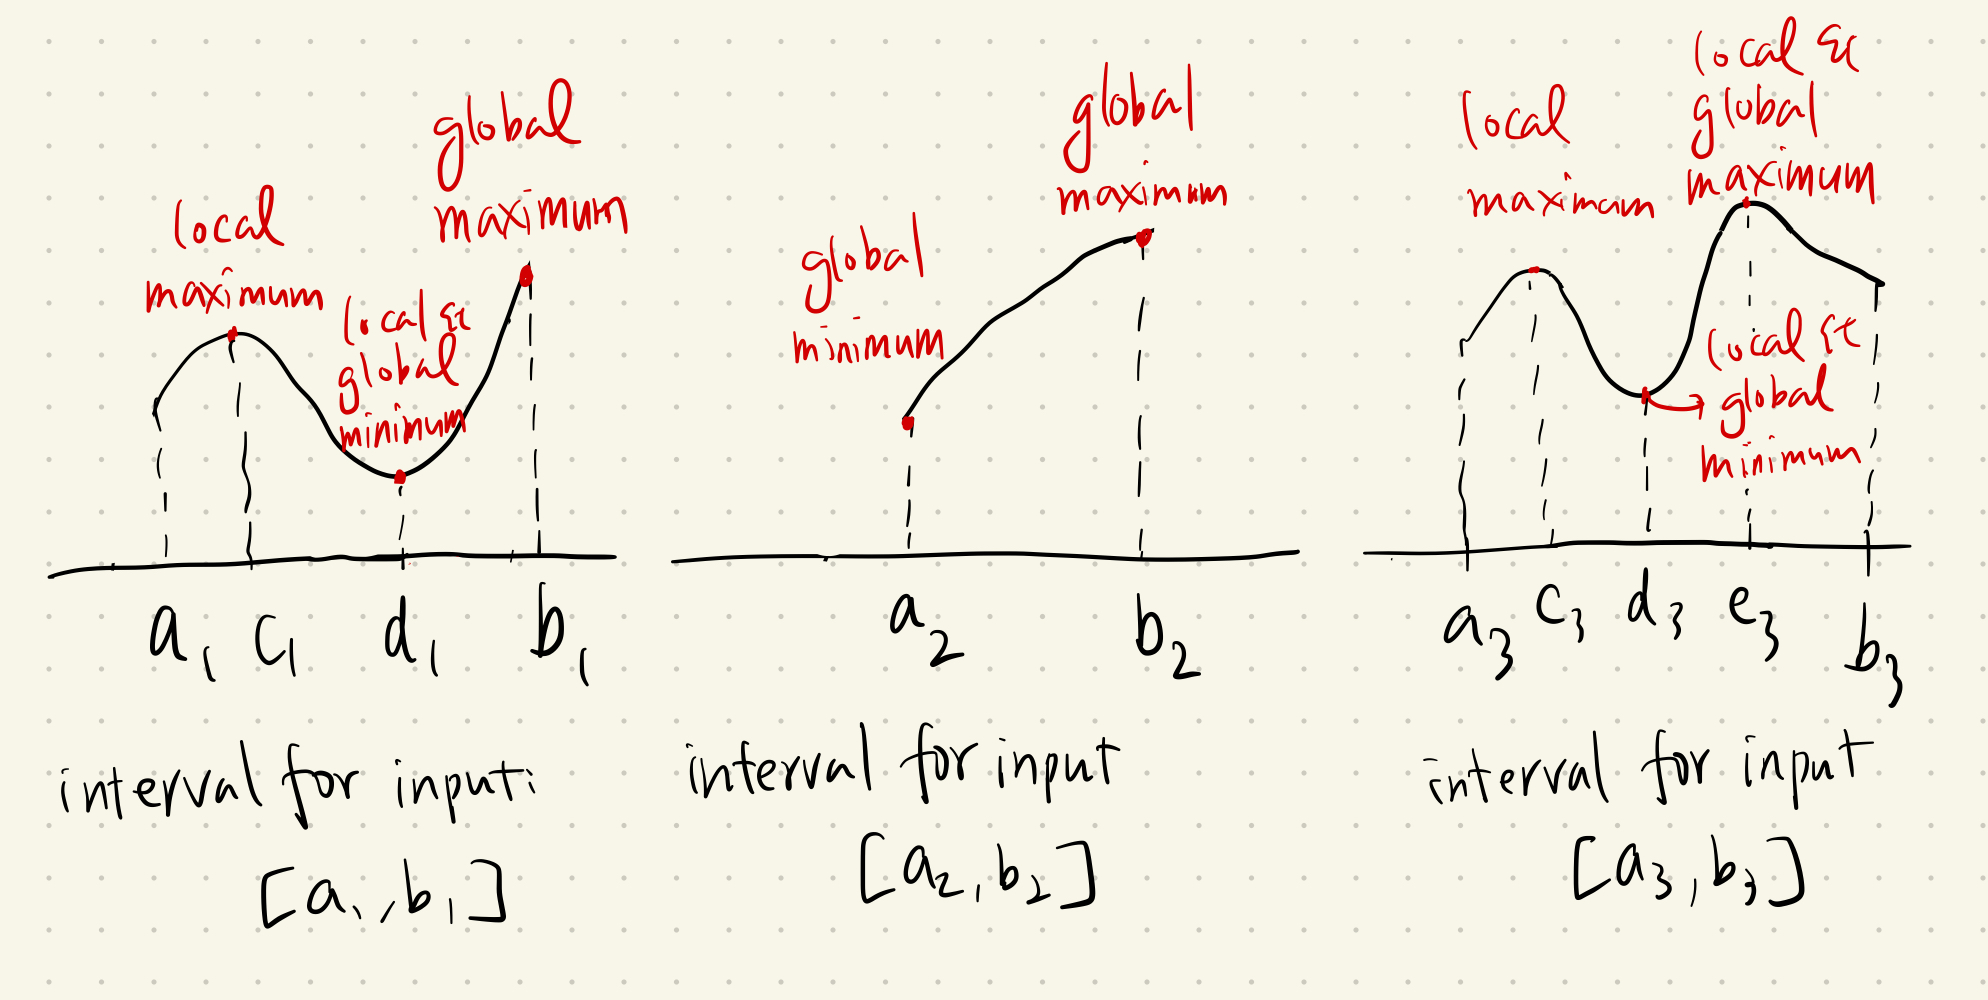
\includegraphics[width = \textwidth]{figures/chap 05/extrema.png}
    \label{fig: extrema}
\end{figure}

We can put these intuition to the test with the graph above:
\begin{itemize}
    \item Left panel: The global maximum is attained at $x=b_1$ since it produces the largest output among inputs within $[a_1, b_1]$.  However, $f(b_1)$ is \textit{not} a local maximum since $b_1$ is at the boundary of $[a_1, b_1]$, so we can't compare $f(b_1)$ with function values evaluated at $x > b_1$.  On the other hand, we have a local maximum attained at $x = c_1$, but it is not a global maximum since $f(c_1) < f(b_1)$.  Local and global extrema can also be attained at the same input, such as $x=d_1$ here where local and global minimum are both attained.
    \item Middle panel: Local extrema do not necessarily exist.  In this example, there are no local extrema for $f(x)$ within $[a_2, b_2]$, but the global extrema still exist.
    \item Right panel: Although there can be at most one global maximum and one global minimum, it is possible to have multiple local maxima or multiple local minima.  In this example, there are two local maxima for $f(x)$ in $[a_3, b_3]$, one attained at $x=c_3$ and the other attained at $x = e_3$.
\end{itemize}

We end this subsection by providing a formal definition of extrema.

\begin{defi}[Extrema]{def: extrema}
    Suppose $x=c$ is in the domain of $f(x)$, let $I_0$ be an interval for input where $c \in I_0$
    \begin{itemize}
        \item $f(x)$ has a \textbf{global (absolute) maximum} at $x=c$ within $I_0$ if $f(x) \le f(c), \forall x \in I_0$ 
        \item $f(x)$ has a \textbf{global (absolute) minimum} at $x=c$ within $I_0$ if $f(x) \ge f(c), \forall x \in I_0$ 
        \\
        \item $f(x)$ has a \textbf{local (relative) maximum} at $x=c$ within $I_0$ if there exists an open interval $I \subset I_0$ where $c \in I$ and $f(x) \le f(c), \forall x \in I$ 
        \item $f(x)$ has a \textbf{local (relative) minimum} at $x=c$ within $I_0$ if there exists an open interval $I \subset I_0$ where $c \in I$ and $f(x) \ge f(c), \forall x \in I$ 
    \end{itemize}
\end{defi}

\subsection{Existence and Identification of Global Extrema}

When we are trying to maximize or minimize a function, what we care about is the \textit{global} extrema.  Therefore, for the maximization or minimization to make sense, we must make sure that the global extrema exist.  However, global extrema do not always exist.  For example, in the following graph, both the global maximum and minimum do not exist.

\begin{figure}[ht]
    \centering
    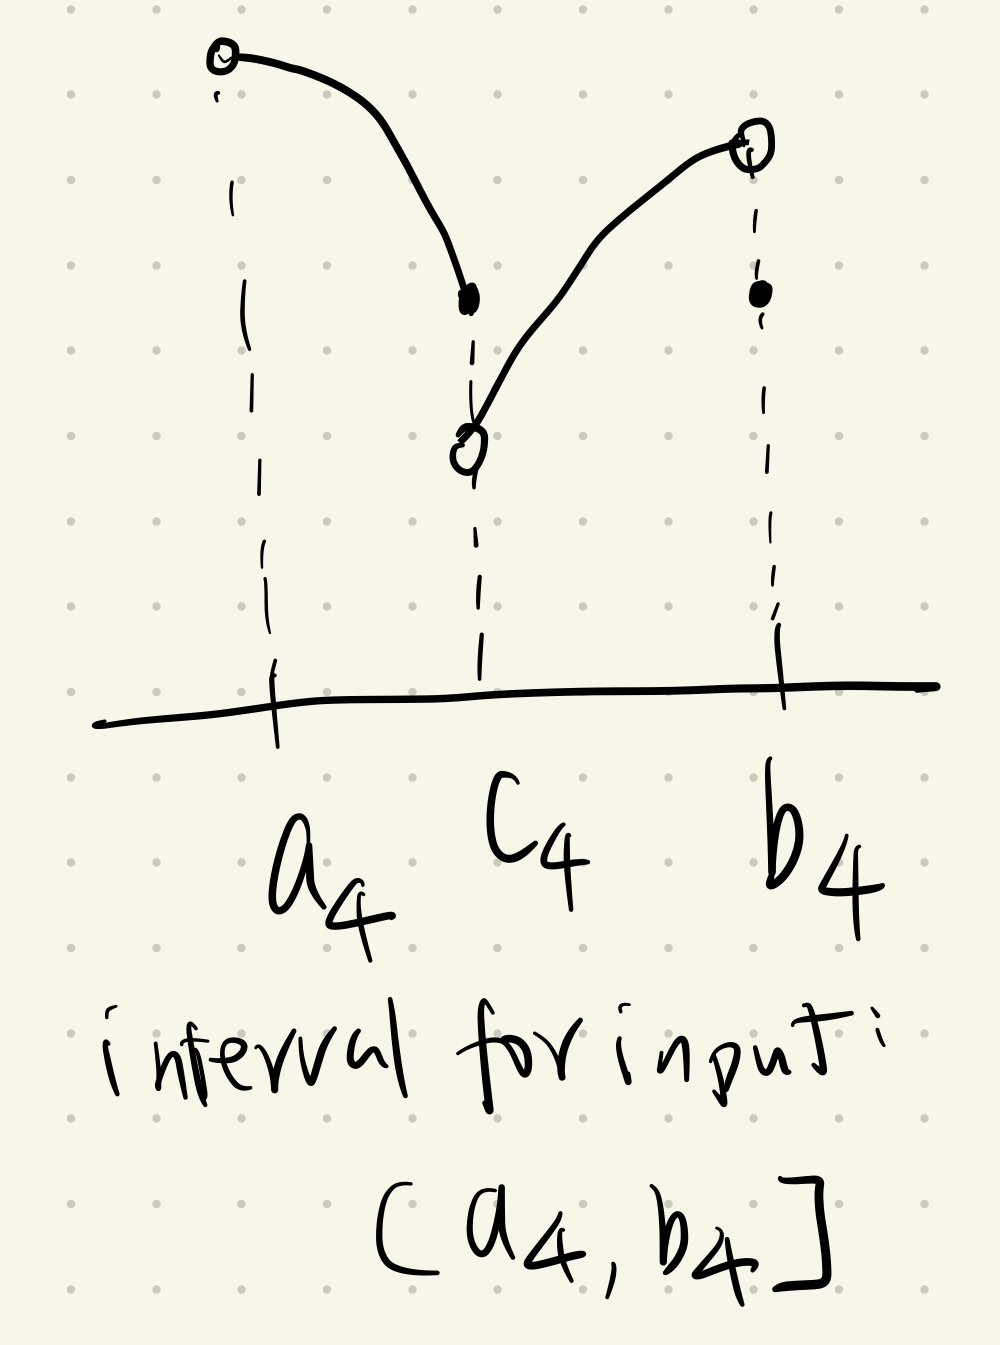
\includegraphics[width = 0.25\textwidth]{figures/chap 05/global_extrema_dne.png}
    \label{fig: global_extrema_dne}
\end{figure}

Fortunately, if we focus on only \textit{continuous} functions with a \textit{closed interval} for input, the global extrema always exists and we can safely do maximization or minimization.  This fact can be summarized in the \textbf{Extreme Value Theorem} below.

\begin{theo}[Extreme Value Theorem]{thm: evt}
    Suppose $f(x)$ is continuous in $[a, b]$, then there exists $x_M, x_m \in [a, b]$ so that $f(x_M)$ is the global maximum of $f(x)$ in $[a, b]$, and $f(x_m)$ is the global minimum of $f(x)$ in $[a, b]$. 
\end{theo}

Now we know the global extrema exist as long as we are dealing with a continuous function within a closed interval for input.  However, knowing their existence is not enough: we want to know where the global extrema is obtained.  To search for global extrema, we first make an important observation: if the global maximum (minimum) is not obtained at the boundaries of the closed interval, then it should also be a local maximum (minimum), since it is larger (smaller) than the function values \textit{around} it.  Therefore, the global extrema can only be attained at the boundaries or at where the local extrema are attained.  This fact is useful since we can locate the local extrema using the following theorem by \textit{Pierre de Fermat}:

\begin{theo}[Fermat's Interior Extremum Theorem]{thm: fermat}
    Suppose $f(x)$ attains local extremum at $x=x_0 \in (a, b)$.  If $f(x)$ is differentiable at $x = x_0$, then $f'(x_0) = 0$.
\end{theo}

An implication of this theorem is that if $f(x)$ has local extremum at $x = x_0$, then either $f'(x_0)=0$ or $f'(x_0)$ does not exist.  Therefore, we can find all candidates of local extremum by identifying all points where the first derivative equals to zero or does not exist, which are the \textit{critical points} of $f(x)$ as we have defined earlier.  An important logic here is that all local extrema occur at critical points, but not all critical points has a local extremum attached to them.  An evident example is $x=x_3$ in Figure~\ref{fig: critical_points}.

Summarizing up, we can find the global extrema of a continuous function $f(x)$ within a close interval $[a, b]$ using the following steps:

\begin{enumerate}
    \setcounter{enumi}{-1}
    \item Verify that $f(x)$ is indeed continuous in $[a, b]$.
    \item Find all the critical points of $f(x)$ in $(a, b)$.
    \item Evaluate $f(x)$ at $a$, $b$, and all the critical points.
    \item Compare the function values: the largest one is the global maximum, and the smallest one is the global minimum.
\end{enumerate}

This procedure is pretty straightforward, which we will demonstrate with a couple of examples. 

\begin{eg}[]{eg: extrema_1}
    Find the global extrema for $f(x) = 2x^3 - 3x^2 - 12x + 5$ in $x \in [-3, 3]$.
\end{eg}

\begin{egsol}[]{egsol: extrema_1}
    We follow the procedure mentioned above:
    \begin{enumerate}
        \setcounter{enumi}{-1}
        \item Since $f(x)$ is a polynomial, it is continuous in $\mathbb{R}$ and thus in $[3, 3]$.
        \item To find the critical points for $f(x)$ in $[-3, 3]$, we first obtain its derivative:
        \[f'(x) = 6x^2-6x-12 = 6(x^2-x-2) = 6(x+1)(x-2)\]
        Therefore, the points where $f'(x) = 0$ are $x = -1$ and $x = 2$, which are both in $[-3, 3]$ and thus our desired critical points.
        \item We evaluate $f(x)$ at $-3, 3, -1, 2$ and yield
        \[f(-3) = -40 \qquad f(3) = -4 \qquad f(-1) = 12 \qquad f(2) = -15\]
        \item Since $-40 = f(-3) < f(2) < f(3) < f(-1) = 12$, the global minimum is $-40$ attained at $x=-3$, and the global maximum is $12$ attained as $x = -1$.
    \end{enumerate}
\end{egsol}

\begin{eg}[]{eg: extrema_2}
    Find the global extrema for $f(x) = 2x + \cos(4x)$ in $x \in \big[-\frac{\pi}{2}, \frac{\pi}{2}\big]$.
\end{eg}

\begin{egsol}[]{egsol: extrema_2}
    We follow the procedure mentioned above:
    \begin{enumerate}
        \setcounter{enumi}{-1}
        \item Since $x$ and $\cos x$ are all continuous in $\mathbb{R}$, $f(x)$ is continuous in $\big[-\frac{\pi}{2}, \frac{\pi}{2}\big]$.
        \item To find the critical points for $f(x)$ in $\big[-\frac{\pi}{2}, \frac{\pi}{2}\big]$, we first obtain its derivative:
        \[f'(x) = 2-4 \sin 4x = 2(1 - 2 \sin 4x)\]
        Therefore, the points where $f'(x) = 0$ are where $\sin 4x = \frac{1}{2}$.  Since $x \in \big[-\frac{\pi}{2}, \frac{\pi}{2}\big]$, we have $4x \in [-2\pi, 2\pi]$, so there are four solutions for $\sin 4x = \frac{1}{2}$: $4x = \frac{\pi}{6}$ or $\frac{5\pi}{6}$ or $\frac{\pi}{6}-2\pi$ or $4x = \frac{5\pi}{6} - 2\pi$.  That is, $x = \frac{\pi}{24}$ or $\frac{5\pi}{24}$ or $-\frac{11\pi}{24}$ or $-\frac{7\pi}{24}$
        \item We evaluate $f(x)$ at $-\frac{\pi}{2}, \frac{\pi}{2}, \frac{\pi}{24}, \frac{5\pi}{24}, -\frac{11\pi}{24}, -\frac{7\pi}{24}$ and yield
        
        \begin{center}
            \begin{tabular}{ll}
                $f\big(-\frac{\pi}{2}\big) = -\pi+1 \approx -2.142$ &  $f\big(\frac{\pi}{2}\big) = \pi+1 \approx 4.142$\\
                $f\big(\frac{\pi}{24}\big) = \frac{\pi}{12} + \frac{\sqrt{3}}{2} \approx 1.128$ & $f\big(\frac{5\pi}{24}\big) = \frac{5\pi}{12} - \frac{\sqrt{3}}{2} \approx 0.443$\\
                $f\big(-\frac{11\pi}{24}\big) = -\frac{11\pi}{12} + \frac{\sqrt{3}}{2} \approx -2.014$ & $ f\big(-\frac{7\pi}{24}\big) = -\frac{7\pi}{12} - \frac{\sqrt{3}}{2} \approx -2.699$
            \end{tabular}
        \end{center}
        \item Since $f\big(-\frac{7\pi}{24}\big) < f\big(-\frac{\pi}{2}\big) < f\big(-\frac{11\pi}{24}\big) < f\big(\frac{5\pi}{24}\big) < f\big(\frac{\pi}{24}\big) < f\big(\frac{\pi}{2}\big)$, the global minimum is $-\frac{7\pi}{12} - \frac{\sqrt{3}}{2}$ attained at $x=-\frac{7\pi}{24}$, and the global maximum is $\pi+1 $ attained as $x = \frac{\pi}{2}$.
    \end{enumerate}
\end{egsol}

\subsection{Identification of Local Extrema}

In the previous subsection, we used Fermat's Interior Extremum Theorem to identify potential points where local extrema may be attained for a function, and concluded that we only needed to look at the critical points of the function.  However, we did not look into the behavior of the function around these critical points.  That is, we do not know if these critical points represent local maximum, local minimum, or neither of them.  As we will show in the next two theorems, we can parse out these scenarios using the function's first and second derivatives, with the intuition brought from what we have learned in curve sketching.

\begin{theo}[First Derivative Test]{thm: first_deriv_test}
    Suppose $x = c$ is a critical point of $f(x)$ where $f'(c) = 0$, then
    \begin{enumerate}
        \item If $f'(x) > 0$ at the left of $x = c$ and $f'(x) < 0$ at the right of $x = c$, then local maximum is attained at $x=c$.
        \item If $f'(x) < 0$ at the left of $x = c$ and $f'(x) > 0$ at the right of $x = c$, then local minimum is attained at $x=c$.
        \item If $f'(x)$ have the same sign on both sides of $x = c$, then $x = c$ does not represent any local extrema.
    \end{enumerate}
\end{theo}

\begin{theo}[Second Derivative Test]{thm: second_deriv_test}
    Suppose $x = c$ is a critical point of $f(x)$ where $f'(c) = 0$ and $f''(x)$ is continuous around $x = c$, then
    \begin{enumerate}
        \item If $f''(c) < 0$, then local maximum is attained at $x=c$.
        \item If $f''(c) > 0$, then local minimum is attained at $x=c$.
        \item If $f''(c) = 0$, then $x = c$ can represent local maximum, local minimum or neither.
    \end{enumerate}
\end{theo}

We look at some examples in the following graph, where $x=0$ is a critical point for all of the functions.  With $y=x^2$ and $y=x^4$, the first derivative is negative when $x<0$ and positive when $x>0$, therefore the function is decreasing when $x < 0$ and increasing when $x > 0$, so $x=0$ represents the position of a local minimum.  Similiar arguments can be  made for $y=-x^2$ and $y=-x^4$, only now $x=0$ represents the position of a local maximum.  For $y = x^3$, the first derivative is positive at both sides of $x=0$, so $x=0$ does not represent local extremum.  

For second derivatives, we see that $y=x^2$ has a positive second derivative at $x=0$, meaning that the function is concave up at $x=0$, so $x=0$ represents a local minimum.  The same can be said for $y=-x^2$.  However, from $y=x^3$, $y=x^4$ and $y=-x^4$ we can see that a second derivative of zero does not give us information on whether $x=0$ represents local maximum, local minimum or neither.  We will have to rely on the first derivative to know for sure.


\begin{figure}[ht]
    \centering
    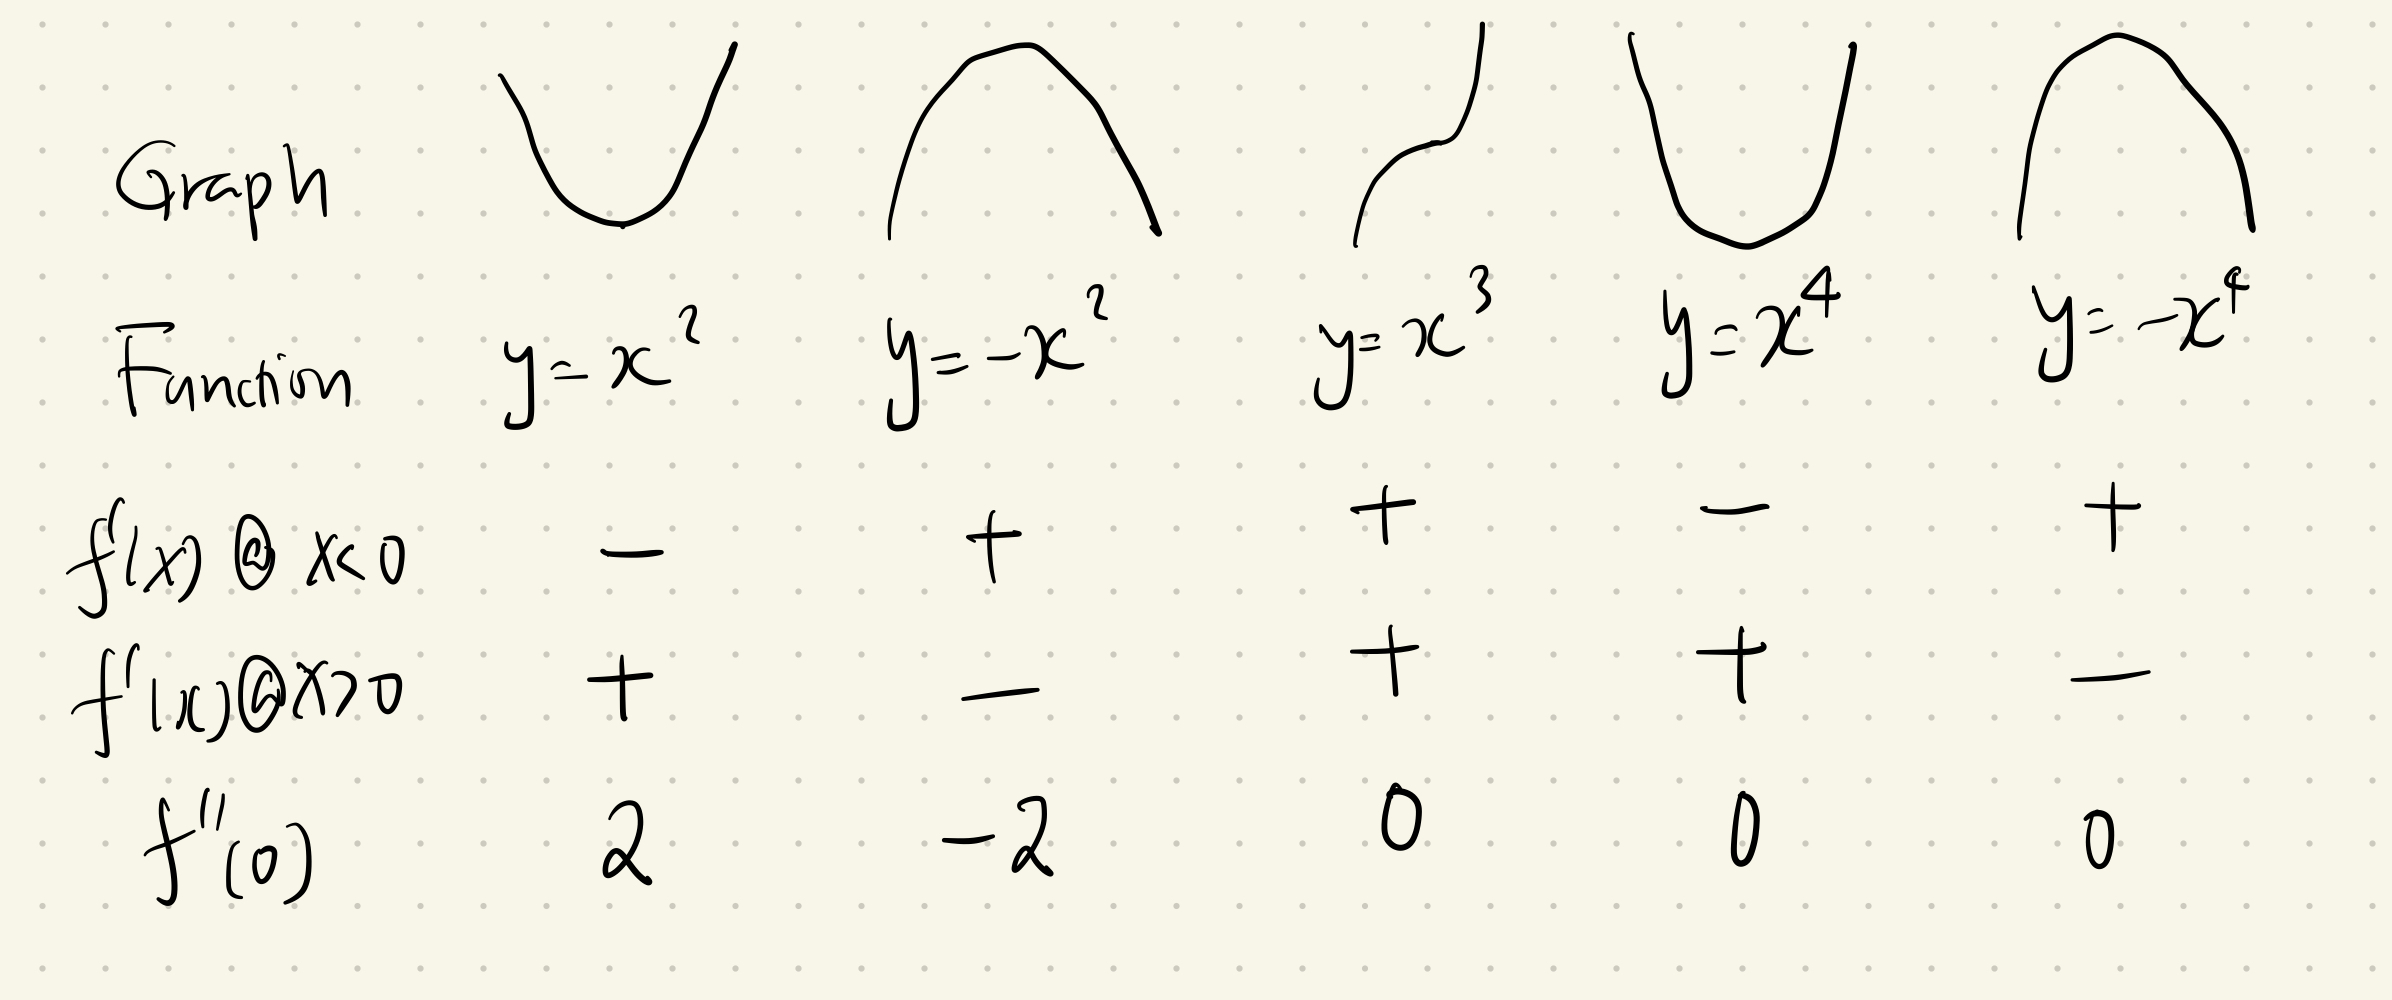
\includegraphics[width = \textwidth]{figures/chap 05/first_second_deriv_test.png}
    \label{fig: first_second_deriv_test}
\end{figure}

We end this section with an example:

\begin{eg}[]{eg: first_second_deriv_test}
    Find all local extrema for $f(x) = 3x^5 - 5x^3 + 30$, and argue if they are local minima or local maxima.
\end{eg}

\begin{egsol}[]{egsol: first_second_deriv_test}
    To locate the local extrema of $f(x)$, we first find the critical points for $f(x)$, which are where $f'(x)$ is undefined or zero.  We first obtain the first derivative:
    \[f'(x) = 15x^4-15x^2 = 15x^2(x^2-1) = 15(x+1)x^2(x-1)\]
    Therefore, we find three critical points for $f(x)$ by letting $f'(x) = 0$, yielding $x= -1$, $0$, or $1$.  Let's now try to identify if they represent local minima, local maxima or neither using the first and second derivative tests.  Note that $f''(x) = 60x^3-30x$.
    \begin{center}
        \begin{tabular}{c|ccccccc}
            $x$ & $(-\infty, -1)$ & $-1$ & $(-1, 0)$ & $0$ & $(0,1)$ & $1$ & $(1, \infty)$  \\
            \hline
            $f'(x)$ & $+$ & $0$ & $-$ & $0$ & $-$ & $0$ & $+$\\
            $f''(x)$ && $-30$ && $0$ && $30$ &
        \end{tabular}
    \end{center}
    We can investigate the three critical points one by one:
    \begin{enumerate}
        \item $x = -1$: The first derivative is positive on the left and negative on the right of $x=-1$, which implies that there is a local maximum here.  This is also confirmed by a negative second derivative at $x = -1$, implying that the curve is concaving down here and this should be a local maximum.
        \item $x = 0$: The first derivative is negative on both sides of $x=0$, which implies this is neither a local maximum nor a local minimum.  The second derivative at $x = 0$ is zero, so it does not provide any information.
        \item $x = 1$, The first derivative is negative on the left and positive on the right of $x=1$, which implies that there is a local minimum here.  This is also confirmed by a positive second derivative at $x = 1$, implying that the curve is concaving up here and this should be a local minimum.
    \end{enumerate}
\end{egsol}

\pagebreak
\section{Optimization Problems}
In the last section, we have shown how to find the maximum or minimum of (i.e. optimize) a function within a given range of input by looking at critical points and boundaries (if the range of input is a closed interval).  In this section, we are trying to use function optimization to solve real-life problems.  The optimization bit remains the same, only that we have to transform our real-life problems into functions we want to optimize and determine the range of input implied by the problem.  Let's get right into it with a few exercises.

\begin{eg}[]{eg: optimization_box}
    A blacksmith wants to craft an open box that has a square base.  Given the amount of material he has, the surface area of the box should be 300 cm$^2$.  What dimensions will produce a box that has the maximum volume?
\end{eg}

\begin{egsol}[]{egsol: optimization_box}
    \begin{center}
        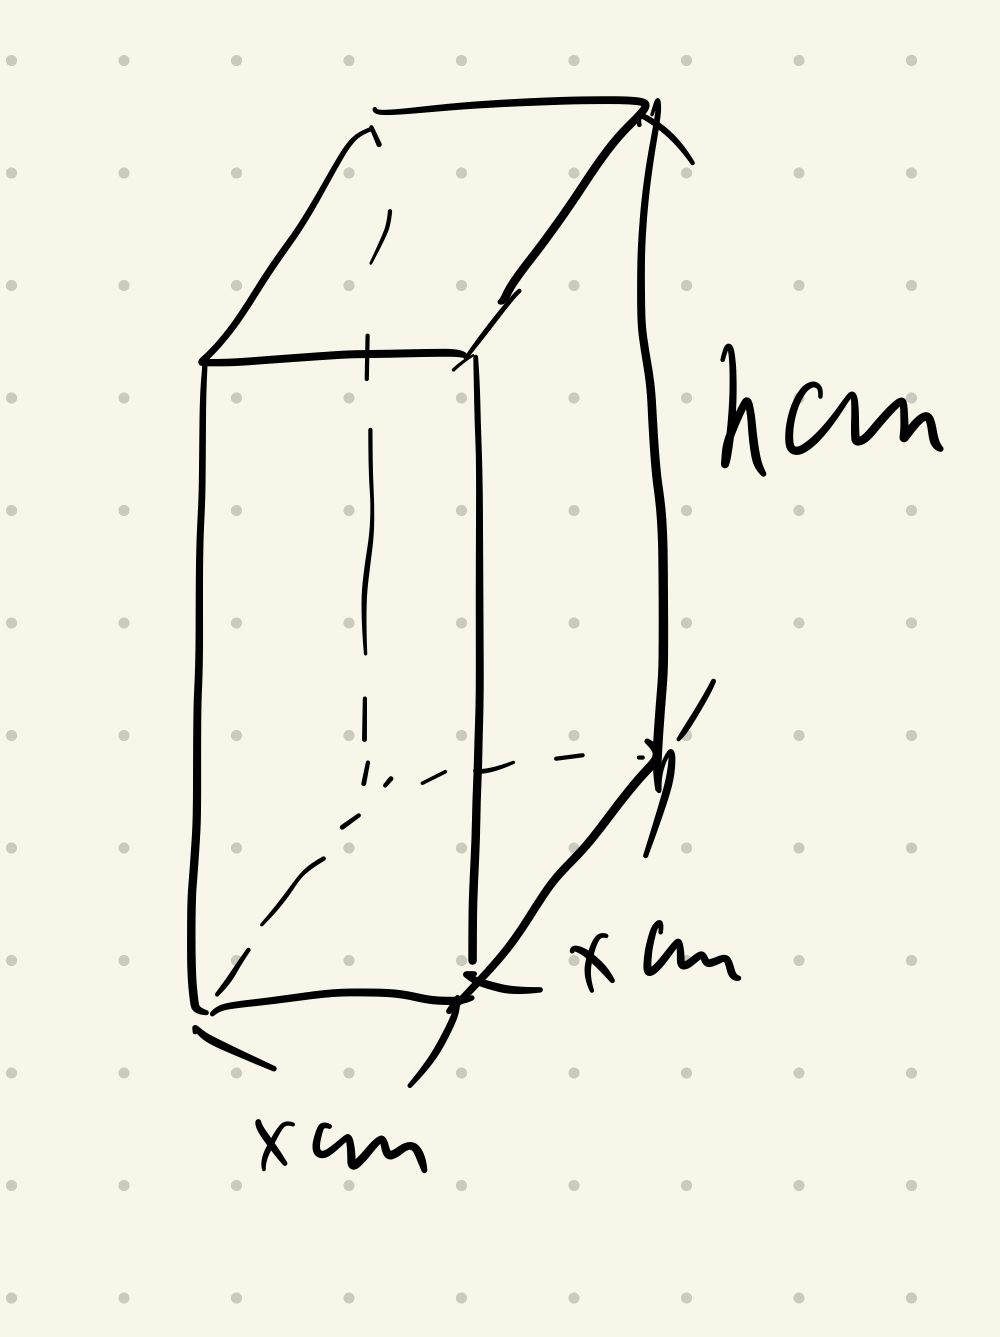
\includegraphics[width = 0.25\textwidth]{figures/chap 05/optimization_box.png}
        \label{fig: ex_optimization_box}
    \end{center}
    Suppose the box has the dimensions above, then we have, from the surface area of the box:
    \[x^2+4xh = 300\]
    Solving for $h$ with $x$ leads us to
    \[h = \frac{300-x^2}{4x}\]
    Therefore, the volume of the box (in cm$^3$), which we are aiming to maximize, is
    \[V := x^2h = x^2\frac{300-x^2}{4x} = 75x-\frac{1}{4}x^3\]
    Note that the possible values of $x$ are restricted by the facts that (1) $x$ refers to the length of the sides for the base, so $x > 0$ (2) $h$ refers to the height of the box, so $h > 0$. $h > 0$ implies that
    \[\frac{300-x^2}{4x} > 0\]
    \[(300-x^2)(4x) > 0\]
    \[(x^2-300)x < 0\]
    \[(x+10\sqrt{3})x(x-10\sqrt{3}) < 0\]
    \[x < -10\sqrt{3} \text{ or } 0 < x < 10\sqrt{3}\]
    Combined with $x > 0$, we have our range of input $x \in (0,10\sqrt{3})$.  To find the global maximum of the volume $V(x) = 75x - \frac{1}{4}x^3$ (which is a continuous function) within $x \in (0, 10\sqrt{3})$, we first find its critical points.  The first derivative of $V(x)$ with respect to $x$ is 
    \[V'(x) = 75 - \frac{3}{4}x^2\]
    Since the first derivative always exists, we find the critical points that make $V'(x) = 0$, which leads to
    \[75-\frac{3}{4}x^2 = 0 \Rightarrow x^2 = 100 \Rightarrow x = \pm 10\]
    Since $x = -10$ is out of the domain $(0, 10\sqrt{3})$, the only critical point is $x = 10$.
    
    To determine if the function is attaining maximum, minimum or neither at $x = 10$, we can use the first derivative test and find that $V'(x) = 75 - \frac{3}{4}x^2$ is positive when $x$ is in $(0, 10)$ and negative when $x$ is in $(10, 10\sqrt{3})$.  Therefore, the volume is attaining both local maximum and global maximum at $x = 10$, with value $V(10) = 500$ (cm$^3$).
    \begin{center}
        \begin{tabular}{cccccc}
            $x$    & $0$ &   & $10$ &   & $10\sqrt{3}$  \\
            \hline
            $V'(x)$ &     & + &      & - & 
        \end{tabular}
    \end{center}
    Another way to show that global maximum is attained at $x = 10$ is to use the second derivative test.  Since $V''(x) = -\frac{3}{2}x$ is always negative in $(0, 10\sqrt{3})$, the function is always concaving down within the range of input, so the critical point $x = 10$ with $V'(x) = 0$ attains both local maximum and global maximum.
\end{egsol}

Note that in the previous example, since the interval of input is an open interval, we cannot verify that $x = 10$ attains global maximum by comparing its function value with the function values at the boundaries as we previously did.  Therefore, we resort to investigating the behavior of the first or second derivative to check the property of the function at $x = 10$.

\begin{ex}[]{ex: optimization_print}
    A poster with a total area of $200$ in$^2$ and has $1$ inch margins on the sides, a $2.5$-inch margin on the top and a $1.5$-inch margin on the bottom. What dimensions will give the largest printed area?
\end{ex}

\begin{exsol}[]{exsol: optimization_print}
    \begin{center}
        \includegraphicsex{width = 0.35\textwidth, draft}{width = 0.35\textwidth}{figures/chap 05/optimization_print.png}
        \label{fig: ex_optimization_print}
    \end{center}
    Suppose the poster is of the dimension as above, then from the total area of the poster, we have
    \[xy = 200 \qquad \Rightarrow \qquad y = \frac{200}{x}\]
    Therefore, the area of the printed area, which we are aiming to maximize, is
    \[A := (x-2)(y-4) = (x-2)\Big(\frac{200}{x}-4\Big) = 200-4x-\frac{400}{x}+8 = 208 - 4x - \frac{400}{x}\]
    Note that the possible values of $x$ are restricted that
    \begin{enumerate}
        \item the width of the printed area must be greater than zero, i.e. $x-2 > 0 \Rightarrow x > 2$
        \item the height of the printed area must be greater than zero, i.e. $y-4 > 0 \Rightarrow \frac{200}{x}>4 \Rightarrow 0 < x < 50$
        \item both $x$ and $y$ stand for lengths, so $x > 0$ and $y > 0 \Rightarrow x > 0$.  
    \end{enumerate}
    
    Combining the above and we yield the range of input for $x$: $(2, 50)$.  To find the global maximum of the volume $A(x) = 208-4x-\frac{400}{x}$ (which is a continuous function) within $x \in (2, 50)$, we first find its critical points.  The first derivative of $A(x)$ with respect to $x$ is 
    \[A'(x) = -4 + \frac{400}{x^2}\]
    Although $A'(x)$ does not exist when $x=0$, this point is not within $(2, 50)$, so it is not a critical point.  We then find the critical points that make $A'(x) = 0$, which leads to
    \[-4 +\frac{400}{x^2} = 0 \Rightarrow x^2 = 100 \Rightarrow x = \pm 10\]
    Since $x = -10$ is out of $(2, 50)$, the only critical point is $x = 10$.
    
    To determine if the function is attaining maximum, minimum or neither at $x = 10$, we use the first derivative test and find that $A'(x) = -4 + \frac{400}{x^2}$ is positive when $x$ is in $(2, 10)$ and negative when $x$ is in $(10, 50)$.  Therefore, the volume is attaining both local maximum and global maximum at $x = 10$, with value $A(10) = 208-40-40 = 128$ (in$^2$).
    \begin{center}
        \begin{tabular}{cccccc}
            $x$    & $2$ &   & $10$ &   & $50$  \\
            \hline
            $A'(x)$ &     & + &      & - & 
        \end{tabular}
    \end{center}
    Another way to show that global maximum is attained at $x = 10$ is to use the second derivative test.  Since $AV''(x) = -\frac{800}{x^3}$ is always negative in $(2, 50)$, the function is always concaving down within the range of input, so the critical point $x = 10$ with $A'(x) = 0$ attains both local maximum and global maximum.
\end{exsol}

\begin{ex}[]{ex: AM-GM}
    Prove the arithmetic mean-geometric mean (AM-GM) inequality: Suppose $x$ and $y$ are both positive, then $\frac{x+y}{2} \ge \sqrt{xy}$, where the equality is attained when $x = y$.
\end{ex}

\begin{exsol}[]{exsol: AM-GM}
    We now try to show that if denote $A := xy$, then $\frac{x+y}{2}$ has a global minimum at $x = y = \sqrt{A}$ with value $\sqrt{A} = \sqrt{xy}$.  Expressing $y$ with $A$ and $x$ and we yield $y = \frac{A}{x}$, and the function we are trying to minimize is $f(x) = \frac{x+A/x}{2}$.  The range of input for $x$ must guarantee (1) $x$ is positive, i.e. $x > 0$ (2) $y$ is positive, i.e. $y = \frac{A}{x} > 0 \Rightarrow x > 0$.  So the combined restriction of input is $x \in (0, \infty)$.
    
    To find the global maximum of the volume $f(x) = \frac{x+A/x}{2}$ (which is a continuous function) within $x \in (0, \infty)$, we first find its critical points.  The first derivative of $f(x)$ with respect to $x$ is 
    \[f'(x) = \frac{1}{2} - \frac{A}{2x^2}\]
    Although $f'(x)$ does not exist when $x=0$, this point is not within $(0, \infty)$, so it is not a critical point.  We then find the critical points that make $f'(x) = 0$, which leads to
    \[\frac{1}{2} - \frac{A}{2x^2} = 0 \Rightarrow x^2 = A \Rightarrow x = \pm \sqrt{A}\]
    Since $x = -\sqrt{A}$ is out of $(0, \infty)$, the only critical point is $x = \sqrt{A}$.
    
    To determine if the function is attaining maximum, minimum or neither at $x = \sqrt{A}$, we use the first derivative test and find that $f'(x) = \frac{1}{2} - \frac{A}{2x^2}$ is negative when $x$ is in $(0, \sqrt{A})$ and positive when $x$ is in $(\sqrt{A}, \infty)$.  Therefore, the function is attaining both local minimum and global minimum at $x = \sqrt{A}$, with value $f(\sqrt{A}) = \sqrt{A}$.
    
    \begin{center}
        \begin{tabular}{ccccc}
            $x$    & $0$ &   & $\sqrt{A}$ &     \\
            \hline
            $f'(x)$ &     & - &      & +
        \end{tabular}
    \end{center}
    
    Therefore, the minimum value $\frac{x+y}{2}$ can attain is $\sqrt{xy}$, where it is attained at $x = y = \sqrt{xy}$.
\end{exsol}